% Options for packages loaded elsewhere
\PassOptionsToPackage{unicode}{hyperref}
\PassOptionsToPackage{hyphens}{url}
\PassOptionsToPackage{dvipsnames,svgnames,x11names}{xcolor}
%
\documentclass[
  bookmarksnumbered]{article}
\usepackage{amsmath,amssymb}
\usepackage{lmodern}
\usepackage{iftex}
\ifPDFTeX
  \usepackage[T1]{fontenc}
  \usepackage[utf8]{inputenc}
  \usepackage{textcomp} % provide euro and other symbols
\else % if luatex or xetex
  \usepackage{unicode-math}
  \defaultfontfeatures{Scale=MatchLowercase}
  \defaultfontfeatures[\rmfamily]{Ligatures=TeX,Scale=1}
\fi
% Use upquote if available, for straight quotes in verbatim environments
\IfFileExists{upquote.sty}{\usepackage{upquote}}{}
\IfFileExists{microtype.sty}{% use microtype if available
  \usepackage[]{microtype}
  \UseMicrotypeSet[protrusion]{basicmath} % disable protrusion for tt fonts
}{}
\makeatletter
\@ifundefined{KOMAClassName}{% if non-KOMA class
  \IfFileExists{parskip.sty}{%
    \usepackage{parskip}
  }{% else
    \setlength{\parindent}{0pt}
    \setlength{\parskip}{6pt plus 2pt minus 1pt}}
}{% if KOMA class
  \KOMAoptions{parskip=half}}
\makeatother
\usepackage{xcolor}
\usepackage[margin=2cm]{geometry}
\usepackage{color}
\usepackage{fancyvrb}
\newcommand{\VerbBar}{|}
\newcommand{\VERB}{\Verb[commandchars=\\\{\}]}
\DefineVerbatimEnvironment{Highlighting}{Verbatim}{commandchars=\\\{\}}
% Add ',fontsize=\small' for more characters per line
\usepackage{framed}
\definecolor{shadecolor}{RGB}{237,237,237}
\newenvironment{Shaded}{\begin{snugshade}}{\end{snugshade}}
\newcommand{\AlertTok}[1]{\textcolor[rgb]{0.75,0.01,0.01}{\textbf{\colorbox[rgb]{0.97,0.90,0.90}{#1}}}}
\newcommand{\AnnotationTok}[1]{\textcolor[rgb]{0.79,0.38,0.79}{#1}}
\newcommand{\AttributeTok}[1]{\textcolor[rgb]{0.00,0.34,0.68}{#1}}
\newcommand{\BaseNTok}[1]{\textcolor[rgb]{0.69,0.50,0.00}{#1}}
\newcommand{\BuiltInTok}[1]{\textcolor[rgb]{0.39,0.29,0.61}{\textbf{#1}}}
\newcommand{\CharTok}[1]{\textcolor[rgb]{0.57,0.30,0.62}{#1}}
\newcommand{\CommentTok}[1]{\textcolor[rgb]{0.54,0.53,0.53}{#1}}
\newcommand{\CommentVarTok}[1]{\textcolor[rgb]{0.00,0.58,1.00}{#1}}
\newcommand{\ConstantTok}[1]{\textcolor[rgb]{0.67,0.33,0.00}{#1}}
\newcommand{\ControlFlowTok}[1]{\textcolor[rgb]{0.12,0.11,0.11}{\textbf{#1}}}
\newcommand{\DataTypeTok}[1]{\textcolor[rgb]{0.00,0.34,0.68}{#1}}
\newcommand{\DecValTok}[1]{\textcolor[rgb]{0.69,0.50,0.00}{#1}}
\newcommand{\DocumentationTok}[1]{\textcolor[rgb]{0.38,0.47,0.50}{#1}}
\newcommand{\ErrorTok}[1]{\textcolor[rgb]{0.75,0.01,0.01}{\underline{#1}}}
\newcommand{\ExtensionTok}[1]{\textcolor[rgb]{0.00,0.58,1.00}{\textbf{#1}}}
\newcommand{\FloatTok}[1]{\textcolor[rgb]{0.69,0.50,0.00}{#1}}
\newcommand{\FunctionTok}[1]{\textcolor[rgb]{0.39,0.29,0.61}{#1}}
\newcommand{\ImportTok}[1]{\textcolor[rgb]{1.00,0.33,0.00}{#1}}
\newcommand{\InformationTok}[1]{\textcolor[rgb]{0.69,0.50,0.00}{#1}}
\newcommand{\KeywordTok}[1]{\textcolor[rgb]{0.12,0.11,0.11}{\textbf{#1}}}
\newcommand{\NormalTok}[1]{\textcolor[rgb]{0.12,0.11,0.11}{#1}}
\newcommand{\OperatorTok}[1]{\textcolor[rgb]{0.12,0.11,0.11}{#1}}
\newcommand{\OtherTok}[1]{\textcolor[rgb]{0.00,0.43,0.16}{#1}}
\newcommand{\PreprocessorTok}[1]{\textcolor[rgb]{0.00,0.43,0.16}{#1}}
\newcommand{\RegionMarkerTok}[1]{\textcolor[rgb]{0.00,0.34,0.68}{\colorbox[rgb]{0.88,0.91,0.97}{#1}}}
\newcommand{\SpecialCharTok}[1]{\textcolor[rgb]{0.24,0.68,0.91}{#1}}
\newcommand{\SpecialStringTok}[1]{\textcolor[rgb]{1.00,0.33,0.00}{#1}}
\newcommand{\StringTok}[1]{\textcolor[rgb]{0.75,0.01,0.01}{#1}}
\newcommand{\VariableTok}[1]{\textcolor[rgb]{0.00,0.34,0.68}{#1}}
\newcommand{\VerbatimStringTok}[1]{\textcolor[rgb]{0.75,0.01,0.01}{#1}}
\newcommand{\WarningTok}[1]{\textcolor[rgb]{0.75,0.01,0.01}{#1}}
\usepackage{longtable,booktabs,array}
\usepackage{calc} % for calculating minipage widths
% Correct order of tables after \paragraph or \subparagraph
\usepackage{etoolbox}
\makeatletter
\patchcmd\longtable{\par}{\if@noskipsec\mbox{}\fi\par}{}{}
\makeatother
% Allow footnotes in longtable head/foot
\IfFileExists{footnotehyper.sty}{\usepackage{footnotehyper}}{\usepackage{footnote}}
\makesavenoteenv{longtable}
\usepackage{graphicx}
\makeatletter
\def\maxwidth{\ifdim\Gin@nat@width>\linewidth\linewidth\else\Gin@nat@width\fi}
\def\maxheight{\ifdim\Gin@nat@height>\textheight\textheight\else\Gin@nat@height\fi}
\makeatother
% Scale images if necessary, so that they will not overflow the page
% margins by default, and it is still possible to overwrite the defaults
% using explicit options in \includegraphics[width, height, ...]{}
\setkeys{Gin}{width=\maxwidth,height=\maxheight,keepaspectratio}
% Set default figure placement to htbp
\makeatletter
\def\fps@figure{htbp}
\makeatother
\setlength{\emergencystretch}{3em} % prevent overfull lines
\providecommand{\tightlist}{%
  \setlength{\itemsep}{0pt}\setlength{\parskip}{0pt}}
\setcounter{secnumdepth}{5}
\newlength{\cslhangindent}
\setlength{\cslhangindent}{1.5em}
\newlength{\csllabelwidth}
\setlength{\csllabelwidth}{3em}
\newlength{\cslentryspacingunit} % times entry-spacing
\setlength{\cslentryspacingunit}{\parskip}
\newenvironment{CSLReferences}[2] % #1 hanging-ident, #2 entry spacing
 {% don't indent paragraphs
  \setlength{\parindent}{0pt}
  % turn on hanging indent if param 1 is 1
  \ifodd #1
  \let\oldpar\par
  \def\par{\hangindent=\cslhangindent\oldpar}
  \fi
  % set entry spacing
  \setlength{\parskip}{#2\cslentryspacingunit}
 }%
 {}
\usepackage{calc}
\newcommand{\CSLBlock}[1]{#1\hfill\break}
\newcommand{\CSLLeftMargin}[1]{\parbox[t]{\csllabelwidth}{#1}}
\newcommand{\CSLRightInline}[1]{\parbox[t]{\linewidth - \csllabelwidth}{#1}\break}
\newcommand{\CSLIndent}[1]{\hspace{\cslhangindent}#1}
\usepackage{setspace} \usepackage{float} \floatplacement{figure}{H} \usepackage[utf8]{inputenc} \usepackage{fancyhdr} \pagestyle{fancy} \lhead{Juan David Leongómez} \rhead{\textit{Meta-análisis de correlaciones en {R:} Guía práctica}} \rfoot{\footnotesize{{doi:} \href{https://doi.org/10.5281/zenodo.5640182}{10.5281/zenodo.5640182}}} \lfoot{\footnotesize{Versión 2}} \renewcommand{\abstractname}{Descripción} \usepackage[spanish]{babel} \usepackage{hanging} \usepackage{amsthm,amssymb,amsfonts} \usepackage{tikz,lipsum,lmodern} \usepackage[most]{tcolorbox} \usepackage{fontawesome5} \usepackage{svg} \usepackage{multirow,booktabs,caption} \renewcommand\spanishtablename{Tabla} \DeclareCaptionLabelSeparator*{spaced}{\\[1ex]} \DeclareCaptionLabelSeparator{point}{. } \captionsetup[table]{labelfont=bf, textfont=it, format=plain, justification=justified, singlelinecheck=false, labelsep=spaced, skip=5pt} \captionsetup[figure]{labelfont=bf, format=plain, justification=justified, singlelinecheck=false,labelsep=point,skip=5pt} \captionsetup[figure]{font=small} \usepackage{orcidlink} \definecolor{iacol}{RGB}{246, 130, 18} \definecolor{iacoldark}{RGB}{246, 100, 18}
\usepackage{booktabs}
\usepackage{longtable}
\usepackage{array}
\usepackage{multirow}
\usepackage{wrapfig}
\usepackage{float}
\usepackage{colortbl}
\usepackage{pdflscape}
\usepackage{tabu}
\usepackage{threeparttable}
\usepackage{threeparttablex}
\usepackage[normalem]{ulem}
\usepackage{makecell}
\usepackage{xcolor}
\ifLuaTeX
  \usepackage{selnolig}  % disable illegal ligatures
\fi
\IfFileExists{bookmark.sty}{\usepackage{bookmark}}{\usepackage{hyperref}}
\IfFileExists{xurl.sty}{\usepackage{xurl}}{} % add URL line breaks if available
\urlstyle{same} % disable monospaced font for URLs
\hypersetup{
  pdftitle={Meta-análisis de correlaciones y meta-regresión en R:},
  pdfauthor={Juan David Leongómez },
  colorlinks=true,
  linkcolor={iacoldark},
  filecolor={Maroon},
  citecolor={Blue},
  urlcolor={blue},
  pdfcreator={LaTeX via pandoc}}

\title{Meta-análisis de correlaciones y meta-regresión en R:}
\usepackage{etoolbox}
\makeatletter
\providecommand{\subtitle}[1]{% add subtitle to \maketitle
  \apptocmd{\@title}{\par {\large #1 \par}}{}{}
}
\makeatother
\subtitle{Guía práctica}
\author{Juan David Leongómez \orcidlink{0000-0002-0092-6298}\textsuperscript{}}
\date{13 marzo, 2023}

\begin{document}
\maketitle

\newtcolorbox[auto counter]{ROut}[2][]{
                lower separated=false,
                colback=white,
                colframe=iacol,
                fonttitle=\bfseries,
                colbacktitle=iacol,
                coltitle=black,
                boxrule=1pt,
                sharp corners,
                breakable,
                enhanced,
                attach boxed title to top left={yshift=-0.1in,xshift=0.15in},
                boxed title style={boxrule=0pt,colframe=white,},
              title=#2,#1}

\begin{center}
\textit{\textbf{EvoCo}: Laboratorio de Evolución y Comportamiento Humano}, Facultad de Psicología, Universidad El Bosque, Bogotá, Colombia. Email: \href{mailto:jleongomez@unbosque.edu.co}{jleongomez@unbosque.edu.co}. Web: \href{https://jdleongomez.info/es}{jdleongomez.info}.

\vfill
\textbf{Resumen}
\end{center}

\par
\begingroup
\leftskip3em
\rightskip\leftskip

El meta-análisis es un método ampliamente utilizado para sintetizar los datos de diferentes estudios. Sin embargo, a menudo estudiantes, profesionales e investigadores carecemos de conocimientos prácticos para hacer e interpretar un meta-análisis. Esta guía presenta una batería de herramientas para realizar meta-análisis de correlaciones en R, ilustradas a partir de un ejemplo real. Incluye desde análisis simples y su interpretación hasta análisis con moderadores (meta-regresión), usando los paquetes \href{https://www.metafor-project.org/doku.php}{\texttt{metafor}} (\protect\hyperlink{ref-viechtbauer2010}{Viechtbauer, 2010}) y \href{https://cran.r-project.org/web/packages/metaviz/vignettes/metaviz.html}{\texttt{metaviz}} (\protect\hyperlink{ref-KossmeierMetaviz}{Kossmeier et al., 2020}). También incluye explicaciones para la transformación de coeficientes \emph{r} de Pearson a \emph{z} de Fisher (y viceversa), creación de gráficos de bosque (\emph{forest plots}) y gráficos de embudo (\emph{funnel plots}), análisis de heterogeneidad y diagnósticos de influencia, así como estrategias para detectar posibles sesgos de publicación utilizando el paquete \href{https://www.r-pkg.org/pkg/weightr}{\texttt{weightr}} (\protect\hyperlink{ref-coburnWeightr2019}{Coburn \& Vevea, 2019}), y para determinar el poder estadístico de un meta-análisis utilizando \href{https://www.dsquintana.blog/metameta-r-package-meta-analysis/}{\texttt{metameta}} (\protect\hyperlink{ref-quintanaMetameta2022}{Quintana, 2022}).

\par
\endgroup

\par
\begingroup
\leftskip3em
\rightskip\leftskip
\footnotesize

\href{https://www.youtube.com/@InvestigacionAbierta}{
\includegraphics{images/Logo-IA-Rectangulo.pdf}}

\textbf{Conocimientos necesarios:} Esta guía asume (1) un manejo básico de R, (2) comprensión de correlaciones y regresiones, y (3) un entendimiento de los principios del meta-análisis. De ser necesario, para adquirir la comprensión básica y necesaria del meta-análisis, recomiendo ver \href{https://youtu.be/ntBbkOn9D_o}{este video} introductorio al meta-análisis en \emph{jamovi} (\protect\hyperlink{ref-leongomezMetaanalysis2021}{Leongómez, 2021}) que publiqué en mi canal de YouTube \href{https://www.youtube.com/@InvestigacionAbierta}{\emph{Investigación Abierta}}.

\textbf{Nota:} Está guía está inspirada en \href{https://youtu.be/lH4VZMTEZSc}{este video} de Quintana (\protect\hyperlink{ref-quintanaHowPerformMetaanalysis2021}{2021}) y sus ejemplos, pero contiene pasos adicionales y alternativos, citas a fuentes primarias, e información complementaria más detallada.

\par
\endgroup
\vfill

\textbf{Cita esta guía como } \hrulefill 

\begin{hangparas}{.25in}{1}
Leongómez, J. D. (2022). Meta-análisis de correlaciones y meta-regresión en R: Guía práctica. \textit{Zenodo}. \url{https://doi.org/10.5281/zenodo.5640182}
\end{hangparas}
\newpage

{\hypersetup{hidelinks}
 \setcounter{tocdepth}{5}
 \tableofcontents
}
\newpage

\hypertarget{base-de-datos-de-ejemplo}{%
\section{Base de datos de ejemplo}\label{base-de-datos-de-ejemplo}}

Para los ejemplos usados en ésta guía, usaré la base de datos \texttt{dat.molloy2014}, tomada de Molloy et al. (\protect\hyperlink{ref-molloy2013}{2013}). Esta base de datos viene incluida con el paquete \texttt{metafor} de R.

Básicamente, Molloy et al. (\protect\hyperlink{ref-molloy2013}{2013}) estudiaron si existe una asociación entre la concienciación (\emph{conscientiousness}\footnote{Para una definición detallada del concepto de concienciación, ver John \& Srivastava (\protect\hyperlink{ref-johnBigFiveTrait1999}{1999}).}) y la adherencia a la medicación. En otras palabras, ¿las personas más \emph{concienciadas} tienden a cumplir más con la medicación prescrita?

Primero, debemos cargar los principales paquetes que usaré a lo largo de esta guía: \texttt{metafor} (\protect\hyperlink{ref-viechtbauer2010}{Viechtbauer, 2010}) y \texttt{metaviz} (\protect\hyperlink{ref-KossmeierMetaviz}{Kossmeier et al., 2020}) para hacer e ilustrar los resultados del meta-análisis, así como \texttt{dplyr} (\protect\hyperlink{ref-WickhamDplyr2021}{Wickham et al., 2021}), \texttt{magrittr} (\protect\hyperlink{ref-magrittrcite}{Bache \& Wickham, 2022}) y \texttt{forecats} (\protect\hyperlink{ref-Wickhamforcats2022}{Wickham, 2022}) para manipular y organizar la base de datos.

\begin{Shaded}
\begin{Highlighting}[]
\FunctionTok{library}\NormalTok{(metafor)}
\FunctionTok{library}\NormalTok{(metaviz)}
\FunctionTok{library}\NormalTok{(dplyr)}
\FunctionTok{library}\NormalTok{(magrittr)}
\FunctionTok{library}\NormalTok{(forcats)}
\end{Highlighting}
\end{Shaded}

Como ya hemos cargado el paquete \texttt{metafor}, ya podemos cargar la base de datos \texttt{dat.molloy2014}. En éste caso, para poder \emph{llamarla} cuando sea necesario, la asignaré a un objeto que llamaré simplemente \texttt{dat}.

\begin{Shaded}
\begin{Highlighting}[]
\NormalTok{dat }\OtherTok{\textless{}{-}} \FunctionTok{get}\NormalTok{(}\FunctionTok{data}\NormalTok{(dat.molloy2014))}
\end{Highlighting}
\end{Shaded}

Tras asignar la base de datos a este objeto (\texttt{dat}), la base de datos se puede ver como \emph{output}\footnote{En R y otros lenguajes de programación, se llama ``\emph{output}'' a la \emph{salida} o resultado visible de una función o proceso, en este caso en la consola (que en RStudio es normalmente el panel que está a la izquierda en la parte inferior).} en la consola de R sencillamente usando como comando el nombre que le dimos al objeto al que lo asignamos (en este caso, \texttt{dat}).

\begin{Shaded}
\begin{Highlighting}[]
\NormalTok{dat}
\end{Highlighting}
\end{Shaded}

\begin{ROut}{Consola de R: Output~\thetcbcounter}
                \begin{footnotesize}
                \begin{verbatim}                authors year  ni     ri controls          design   a_measure
1      Axelsson et al. 2009 109  0.187     none cross-sectional self-report
2      Axelsson et al. 2011 749  0.162     none cross-sectional self-report
3         Bruce et al. 2010  55  0.340     none     prospective       other
4   Christensen et al. 1999 107  0.320     none cross-sectional self-report
5  Christensen & Smith 1995  72  0.270     none     prospective       other
6         Cohen et al. 2004  65  0.000     none     prospective       other
7       Dobbels et al. 2005 174  0.175     none cross-sectional self-report
8        Ediger et al. 2007 326  0.050 multiple     prospective self-report
9         Insel et al. 2006  58  0.260     none     prospective       other
10       Jerant et al. 2011 771  0.010 multiple     prospective       other
11        Moran et al. 1997  56 -0.090 multiple     prospective       other
12   O'Cleirigh et al. 2007  91  0.370     none     prospective self-report
13       Penedo et al. 2003 116  0.000     none cross-sectional self-report
14        Quine et al. 2012 537  0.150     none     prospective self-report
15      Stilley et al. 2004 158  0.240     none     prospective       other
16 Wiebe & Christensen 1997  65  0.040     none     prospective       other
   c_measure meanage quality
1      other   22.00       1
2        NEO   53.59       1
3        NEO   43.36       2
4      other   41.70       1
5        NEO   46.39       2
6        NEO   41.20       2
7        NEO   52.30       1
8        NEO   41.00       3
9      other   77.00       2
10       NEO   78.60       3
11       NEO   57.20       2
12       NEO   37.90       2
13       NEO   39.20       1
14     other   69.00       2
15       NEO   46.20       3
16       NEO   56.00       1
 \end{verbatim}
                \end{footnotesize}
                \end{ROut}

\hypertarget{variables-de-la-base-de-datos}{%
\subsection{Variables de la base de datos}\label{variables-de-la-base-de-datos}}

Por favor mira la base de datos, y familiarízate con sus columnas. ¿Qué información contiene cada variable? Explicaré cada una a continuación.

Primero, hay unas columnas que contienen información absolutamente necesaria para poder hacer un meta-análisis:

\begin{itemize}
\item
  \texttt{authors}: los autores de cada estudio a meta-analizar
\item
  \texttt{year}: año de publicación de cada estudio
\item
  \texttt{ni}: tamaño de muestra de cada estudio
\item
  \texttt{ri}: coeficiente de correlación de Pearson de cada estudio
\end{itemize}

Esas son las variables más importantes y son necesarias para hacer un meta-análisis de correlación simple: alguna columna o columnas con información que permita identificar cada estudio (en este caso \texttt{authors} y \texttt{year}), una columna con el tamaño de muestra de cada estudio (en este caso, \texttt{ni}), y finalmente una columna con los coeficientes de correlación (en este caso la columna \texttt{ri}). Si tu meta-análisis no requiere moderadores, con una estructura como esta sería suficiente.

Después hay unas columnas que contienen variables específicas para este este ejemplo, y que son una serie de posibles moderadores que agrupan características de los estudios a meta-analizar:

\begin{itemize}
\item
  \texttt{controls}: cantidad de variables controladas (``\texttt{none}'': ninguna o ``\texttt{multiple}'': múltiples)
\item
  \texttt{design}: si se utilizó un diseño transversal (``\texttt{cross-section}'') o prospectivo (``\texttt{prospective}'') (para más información acerca de estos tipos de diseño, ver por ejemplo \protect\hyperlink{ref-Manterola2019}{Manterola et al., 2019})
\item
  \texttt{a\_measure}: tipo de medida de adherencia (``\texttt{self-report}'': autoinforme u ``\texttt{other}'': otro tipo de medida más \emph{objetivo})
\item
  \texttt{c\_measure}: tipo de medida de concienciación (si se midió con alguna versión del inventario de personalidad NEO o con alguna otra escala)
\item
  \texttt{meanage}: edad promedio de la muestra de cada estudio
\item
  \texttt{quality}: calidad metodológica (la calidad metodológica fue calificada por los autores del meta-análisis en una escala de 1 a 4, donde las puntuaciones más altas indican una mayor calidad; para información respecto a cómo se obtuvo esta puntuación, ver el artículo original de Molloy et al. (\protect\hyperlink{ref-molloy2013}{2013}).
\end{itemize}

Por supuesto, el \emph{output} de la consola no es la forma más clara de ver la base de datos, pero para una versión más legible, se puede usar la función \texttt{View}, y el nombre de la base de datos o tabla como argumento (en este caso \texttt{View(dat)}). Sin embargo, de aquí en adelante mostraré algunas tablas en un formato de impresión (y no como sale en la consola de R), para que sean más fáciles de leer.

Voy a volver a cargar la base de datos (sobrescribiendo el objeto \texttt{dat}), para organizarla un poco mejor. Primero, agregaré una nueva columna llamada \texttt{study\_id}, en la que numeraré los estudios del 1 al 16, lo que será útil para identificar cada estudio en algunas gráficas y análisis. Después, reorganizaré las columnas para que \texttt{study\_id} sea la primera, en vez de la última columna. Finalmente, las columnas de variables que son factores (\texttt{controls}, \texttt{design}, \texttt{a\_measure}, \texttt{c\_measure} y \texttt{quality}), pueden ser definidas como tal, para evitar pasos adicionales más adelante. En este caso, .

\begin{Shaded}
\begin{Highlighting}[]
\NormalTok{dat }\OtherTok{\textless{}{-}} \FunctionTok{get}\NormalTok{(}\FunctionTok{data}\NormalTok{(dat.molloy2014)) }\SpecialCharTok{\%\textgreater{}\%}
  \FunctionTok{mutate}\NormalTok{(}\AttributeTok{study\_id =} \DecValTok{1}\SpecialCharTok{:}\DecValTok{16}\NormalTok{)  }\SpecialCharTok{\%\textgreater{}\%} \CommentTok{\#crear columna study\_id y agregar números del 1 al 16}
  \FunctionTok{select}\NormalTok{(study\_id, authors}\SpecialCharTok{:}\NormalTok{quality) }\SpecialCharTok{\%\textgreater{}\%} \CommentTok{\#mover study\_id como primera columna}
  \FunctionTok{mutate\_at}\NormalTok{(}\FunctionTok{c}\NormalTok{(}\StringTok{"controls"}\NormalTok{, }\CommentTok{\# Transformar variables en factores}
              \StringTok{"design"}\NormalTok{,}
              \StringTok{"a\_measure"}\NormalTok{,}
              \StringTok{"c\_measure"}\NormalTok{,}
              \StringTok{"quality"}\NormalTok{), }
\NormalTok{            as.factor) }\SpecialCharTok{\%\textgreater{}\%} 
  \FunctionTok{mutate}\NormalTok{(}\AttributeTok{controls =} \FunctionTok{fct\_relevel}\NormalTok{(controls, }\StringTok{"none"}\NormalTok{, }\StringTok{"multiple"}\NormalTok{))}
\end{Highlighting}
\end{Shaded}

Con esto, la base de datos tiene ahora la siguiente estructura (Tabla \ref{tab:estructuramod}):

\begin{table}[H]

\caption{\label{tab:estructuramod}Estructura de la base de datos con estudios numerados}
\centering
\resizebox{\linewidth}{!}{
\begin{tabular}[t]{rlrrrllllrl}
\toprule
study\_id & authors & year & ni & ri & controls & design & a\_measure & c\_measure & meanage & quality\\
\midrule
1 & Axelsson et al. & 2009 & 109 & 0.187 & none & cross-sectional & self-report & other & 22.00 & 1\\
2 & Axelsson et al. & 2011 & 749 & 0.162 & none & cross-sectional & self-report & NEO & 53.59 & 1\\
3 & Bruce et al. & 2010 & 55 & 0.340 & none & prospective & other & NEO & 43.36 & 2\\
4 & Christensen et al. & 1999 & 107 & 0.320 & none & cross-sectional & self-report & other & 41.70 & 1\\
5 & Christensen \& Smith & 1995 & 72 & 0.270 & none & prospective & other & NEO & 46.39 & 2\\
6 & Cohen et al. & 2004 & 65 & 0.000 & none & prospective & other & NEO & 41.20 & 2\\
7 & Dobbels et al. & 2005 & 174 & 0.175 & none & cross-sectional & self-report & NEO & 52.30 & 1\\
8 & Ediger et al. & 2007 & 326 & 0.050 & multiple & prospective & self-report & NEO & 41.00 & 3\\
9 & Insel et al. & 2006 & 58 & 0.260 & none & prospective & other & other & 77.00 & 2\\
10 & Jerant et al. & 2011 & 771 & 0.010 & multiple & prospective & other & NEO & 78.60 & 3\\
11 & Moran et al. & 1997 & 56 & -0.090 & multiple & prospective & other & NEO & 57.20 & 2\\
12 & O'Cleirigh et al. & 2007 & 91 & 0.370 & none & prospective & self-report & NEO & 37.90 & 2\\
13 & Penedo et al. & 2003 & 116 & 0.000 & none & cross-sectional & self-report & NEO & 39.20 & 1\\
14 & Quine et al. & 2012 & 537 & 0.150 & none & prospective & self-report & other & 69.00 & 2\\
15 & Stilley et al. & 2004 & 158 & 0.240 & none & prospective & other & NEO & 46.20 & 3\\
16 & Wiebe \& Christensen & 1997 & 65 & 0.040 & none & prospective & other & NEO & 56.00 & 1\\
\bottomrule
\multicolumn{11}{l}{\rule{0pt}{1em}\textit{Nota:} Datos tomados de Molloy et al. (2013).}\\
\end{tabular}}
\end{table}

\hypertarget{preparaciuxf3n-de-los-datos-transformaciuxf3n-de-coeficientes-r-de-pearson-a-z-de-fisher}{%
\section{\texorpdfstring{Preparación de los datos: transformación de coeficientes \emph{r} de Pearson a \emph{z} de Fisher}{Preparación de los datos: transformación de coeficientes r de Pearson a z de Fisher}}\label{preparaciuxf3n-de-los-datos-transformaciuxf3n-de-coeficientes-r-de-pearson-a-z-de-fisher}}

Los coeficientes de Pearson no se distribuyen normalmente, lo que podría llevar a calcular varianzas incorrectas, especialmente cuando se trata de correlaciones con tamaños de muestra pequeños. Por esto, lo mejor es transformar los coeficientes \emph{r} de Pearson a \emph{z} de Fisher (\protect\hyperlink{ref-fisherFrequencyDistributionValues1915}{Fisher, 1915}), que no tienen este problema\footnote{Para decirlo de manera más precisa, el problema es que la distribución del coeficiente de correlación de Pearson (\emph{r}), es muy sesgada cuando se trata de variables altamente correlacionadas (positiva, o negativamente). Esto dificulta la estimación de los intervalos de confianza y por tanto la aplicación de las pruebas de significación para coeficientes \emph{r}. La transformación de Fisher de valores \emph{r} a \emph{z} ---que es la \href{https://es.wikipedia.org/wiki/Tangente_hiperb\%C3\%B3lica}{tangente hiperbólica inversa} de \emph{r}--- resuelve este problema, pues los coeficientes \emph{z} tienen una distribución aproximadamente normal, y una varianza estable a lo largo de diferentes valores posibles de \emph{r} (para una demostración en español, ver \protect\hyperlink{ref-sanchez-brunoTransformacionFisherPara2005}{Sánchez-Bruno \& Borges del Rosal, 2005}).}.

Para transformar los coeficientes \emph{r} de Pearson a coeficientes \emph{z} de Fisher, usaré la función \texttt{escalc} del paquete \texttt{metafor}, que sirve para calcular diversos tamaños de efecto que se utilizan comúnmente en meta-análisis. Los argumentos que requiere esta función, además del tipo de transformación a realizar (en este caso \texttt{measure\ =\ "ZCOR"}), son los coeficientes de correlación (\texttt{ri}), el tamaño de muestra de cada correlación (\texttt{ni}), y la base de datos que contiene estos valores (\texttt{data}). En nuestro caso, las columnas donde están estos valores, tienen los mismos nombres (\texttt{ri}, \texttt{ni}). En este ejemplo, asignaré el resultado de esta función al mismo objeto \texttt{dat}, que contiene la base de datos, para sobrescribirlo y no crear objetos adicionales.

\begin{Shaded}
\begin{Highlighting}[]
\NormalTok{dat }\OtherTok{\textless{}{-}} \FunctionTok{escalc}\NormalTok{(}\AttributeTok{measure =} \StringTok{"ZCOR"}\NormalTok{, }\AttributeTok{ri =}\NormalTok{ ri, }\AttributeTok{ni =}\NormalTok{ ni, }\AttributeTok{data =}\NormalTok{ dat)}
\end{Highlighting}
\end{Shaded}

Esta función agrega dos nuevas variables: \texttt{yi}, que es el tamaño de efecto (en valores \emph{z} de Fisher), y \texttt{vi} que es la varianza (Tabla \ref{tab:estructuramod2}).

\begin{table}[H]

\caption{\label{tab:estructuramod2}Estructura de la base de datos, con transformación de los r de Pearon a z de Fisher}
\centering
\resizebox{\linewidth}{!}{
\begin{tabular}[t]{rlrrrllllrl>{}r>{}r}
\toprule
study\_id & authors & year & ni & ri & controls & design & a\_measure & c\_measure & meanage & quality & yi & vi\\
\midrule
1 & Axelsson et al. & 2009 & 109 & 0.187 & none & cross-sectional & self-report & other & 22.00 & 1 & \cellcolor[HTML]{f68212}{0.1892266} & \cellcolor[HTML]{f68212}{0.0094340}\\
2 & Axelsson et al. & 2011 & 749 & 0.162 & none & cross-sectional & self-report & NEO & 53.59 & 1 & \cellcolor[HTML]{f68212}{0.1634399} & \cellcolor[HTML]{f68212}{0.0013405}\\
3 & Bruce et al. & 2010 & 55 & 0.340 & none & prospective & other & NEO & 43.36 & 2 & \cellcolor[HTML]{f68212}{0.3540925} & \cellcolor[HTML]{f68212}{0.0192308}\\
4 & Christensen et al. & 1999 & 107 & 0.320 & none & cross-sectional & self-report & other & 41.70 & 1 & \cellcolor[HTML]{f68212}{0.3316471} & \cellcolor[HTML]{f68212}{0.0096154}\\
5 & Christensen \& Smith & 1995 & 72 & 0.270 & none & prospective & other & NEO & 46.39 & 2 & \cellcolor[HTML]{f68212}{0.2768638} & \cellcolor[HTML]{f68212}{0.0144928}\\
6 & Cohen et al. & 2004 & 65 & 0.000 & none & prospective & other & NEO & 41.20 & 2 & \cellcolor[HTML]{f68212}{0.0000000} & \cellcolor[HTML]{f68212}{0.0161290}\\
7 & Dobbels et al. & 2005 & 174 & 0.175 & none & cross-sectional & self-report & NEO & 52.30 & 1 & \cellcolor[HTML]{f68212}{0.1768200} & \cellcolor[HTML]{f68212}{0.0058480}\\
8 & Ediger et al. & 2007 & 326 & 0.050 & multiple & prospective & self-report & NEO & 41.00 & 3 & \cellcolor[HTML]{f68212}{0.0500417} & \cellcolor[HTML]{f68212}{0.0030960}\\
9 & Insel et al. & 2006 & 58 & 0.260 & none & prospective & other & other & 77.00 & 2 & \cellcolor[HTML]{f68212}{0.2661084} & \cellcolor[HTML]{f68212}{0.0181818}\\
10 & Jerant et al. & 2011 & 771 & 0.010 & multiple & prospective & other & NEO & 78.60 & 3 & \cellcolor[HTML]{f68212}{0.0100003} & \cellcolor[HTML]{f68212}{0.0013021}\\
11 & Moran et al. & 1997 & 56 & -0.090 & multiple & prospective & other & NEO & 57.20 & 2 & \cellcolor[HTML]{f68212}{-0.0902442} & \cellcolor[HTML]{f68212}{0.0188679}\\
12 & O'Cleirigh et al. & 2007 & 91 & 0.370 & none & prospective & self-report & NEO & 37.90 & 2 & \cellcolor[HTML]{f68212}{0.3884231} & \cellcolor[HTML]{f68212}{0.0113636}\\
13 & Penedo et al. & 2003 & 116 & 0.000 & none & cross-sectional & self-report & NEO & 39.20 & 1 & \cellcolor[HTML]{f68212}{0.0000000} & \cellcolor[HTML]{f68212}{0.0088496}\\
14 & Quine et al. & 2012 & 537 & 0.150 & none & prospective & self-report & other & 69.00 & 2 & \cellcolor[HTML]{f68212}{0.1511404} & \cellcolor[HTML]{f68212}{0.0018727}\\
15 & Stilley et al. & 2004 & 158 & 0.240 & none & prospective & other & NEO & 46.20 & 3 & \cellcolor[HTML]{f68212}{0.2447741} & \cellcolor[HTML]{f68212}{0.0064516}\\
16 & Wiebe \& Christensen & 1997 & 65 & 0.040 & none & prospective & other & NEO & 56.00 & 1 & \cellcolor[HTML]{f68212}{0.0400214} & \cellcolor[HTML]{f68212}{0.0161290}\\
\bottomrule
\multicolumn{13}{l}{\rule{0pt}{1em}\textit{Nota:} Las nuevas columnas creadas usando la función \texttt{escalc} 
           (\texttt{yi} como tamaño de efecto y \texttt{vi} como varianza) están 
           resaltadas en naranja}\\
\end{tabular}}
\end{table}

\hypertarget{meta-cor}{%
\section{Hacer el meta-análisis}\label{meta-cor}}

Para hacer el meta-análisis, usaré la función \texttt{rma} del paquete \texttt{metafor}. Esta función requiere especificar los tamaños de efecto (\texttt{yi}) y varianzas (\texttt{vi}) de los estudios a meta-analizar. En nuestro caso, las columnas donde están estos valores, tienen los mismos nombres (\texttt{yi}, \texttt{vi}). Asignaré los resultados del meta-análisis a un nuevo objeto llamado \texttt{res}.

\begin{Shaded}
\begin{Highlighting}[]
\NormalTok{res }\OtherTok{\textless{}{-}} \FunctionTok{rma}\NormalTok{(}\AttributeTok{yi =}\NormalTok{ yi, }\AttributeTok{vi =}\NormalTok{ vi, }\AttributeTok{data =}\NormalTok{ dat)}
\end{Highlighting}
\end{Shaded}

Los resultados, son los siguientes:

\begin{Shaded}
\begin{Highlighting}[]
\NormalTok{res}
\end{Highlighting}
\end{Shaded}

\begin{ROut}{Consola de R: Output~\thetcbcounter}
                \begin{footnotesize}
                \begin{verbatim} 
Random-Effects Model (k = 16; tau^2 estimator: REML)

tau^2 (estimated amount of total heterogeneity): 0.0081 (SE = 0.0055)
tau (square root of estimated tau^2 value):      0.0901
I^2 (total heterogeneity / total variability):   61.73%
H^2 (total variability / sampling variability):  2.61

Test for Heterogeneity:
Q(df = 15) = 38.1595, p-val = 0.0009

Model Results:

estimate      se    zval    pval   ci.lb   ci.ub      
  0.1499  0.0316  4.7501  <.0001  0.0881  0.2118  *** 

---
Signif. codes:  0 '***' 0.001 '**' 0.01 '*' 0.05 '.' 0.1 ' ' 1
 \end{verbatim}
                \end{footnotesize}
                \end{ROut}

\hypertarget{meta-interp}{%
\subsection{Interpretación de los resultados del meta-análisis}\label{meta-interp}}

Vamos a analizar estos resultados de la consola de R por partes:

Primero, nos confirman que ajustamos un modelo con efectos aleatorios (\texttt{Random-Effects\ Model}), a partir de 16 estudios (\texttt{k\ =\ 16}), y que para estimar \(\tau^2\) (tau cuadrado) usamos el método de \textbf{máxima verosimilitud restringida}\footnote{Hay varios métodos disponibles como estimador, además de \textbf{máxima verosimilitud restringida} (REML). Sin embargo, si tienes dudas, REML es una buena opción. Cada método tiene ventajas y desventajas que, si tienes interés en mirar, están descritas en la \href{https://www.rdocumentation.org/packages/metafor/versions/2.4-0/topics/rma.uni}{documentación} de la función \texttt{rma}.} (\texttt{tau\^{}2\ estimator:\ REML}), que se designa como \emph{REML} por sus siglas en inglés .

Posteriormente, nos provee los valores de una serie de estimadores de heterogeneidad:

\begin{itemize}
\item
  \(\tau^2\): \texttt{tau\^{}2\ (estimated\ amount\ of\ total\ heterogeneity):\ 0.0081\ (SE\ =\ 0.0055)}
\item
  \(\tau\): \texttt{tau\ (square\ root\ of\ estimated\ tau\^{}2\ value):\ 0.0901}
\item
  \(I^2\): \texttt{I\^{}2\ (total\ heterogeneity\ /\ total\ variability):\ 61.73\%}, y
\item
  \(H^2\): \texttt{H\^{}2\ (total\ variability\ /\ sampling\ variability):\ \ 2.61}
\end{itemize}

La tercera parte, reporta otra prueba de heterogeneidad, usando el estadístico \(Q\):

\begin{itemize}
\item
  \texttt{Test\ for\ Heterogeneity:}

  \texttt{Q(df\ =\ 15)\ =\ 38.1595,\ p-val\ =\ 0.0009}
\end{itemize}

De todos estos, los más comúnmente reportados son \(\tau^2\), \(\tau\), \(I^2\) y \(Q\). Cada una de estas medidas tiene ventajas y desventajas, por lo cual tiene sentido reportarlas todas.

\begin{itemize}
\item
  \(I^2\): tiene la ventaja de ser sencillo de interpretar, pues hay criterios generales para heterogeneidad baja, moderada y alta (típicamente 25\%, 50\%, and 75\%, respectivamente). Sin embargo, es muy sensible a los tamaños de muestra de los estudios meta-analizados (por ejemplo, si en tu meta-análisis hay estudios con tamaños de muestra muy grandes, esto va a sesgar tu \(I^2\)).
\item
  \(Q\): aunque no es sensible al tamaño de muestra, es sensible al número de estudios meta-analizados. Tiene la ventaja de ser un test de hipótesis, y como tal, puede ser interpretado a partir de su valor \emph{p}.
\item
  \(\tau^2\): no tiene problemas de sensibilidad a los tamaños de muestra o número de estudios meta-analizados, pero es más difícil de interpretar. \(\tau^2\) es una estimación de la varianza de los tamaños de los efectos reales entre los estudios meta-analizados. Se usa, principalmente, para asignar pesos a cada estudio (para más información, ver \protect\hyperlink{ref-borensteinIdentifyingQuantifyingHeterogeneity2009}{Borenstein et al., 2009}).
\end{itemize}

En nuestro caso, el estadístico \(Q\) sugiere que hay una heterogeneidad significativa en los estudios meta-analizados (\(p\) = 0.0009). \(I^2\), sugiere una heterogeneidad moderada, lo que quiere decir que se estima que más de la mitad (61.73\%) de la varianza se deriva de diferencias en los tamaños de efecto.

Más abajo, el \emph{output} de la consola de R nos muestra los resultados de nuestro meta-análisis (\texttt{Model\ results}); en otras palabras, ¿cuál es el tamaño de efecto de la asociación entre concienciación (\emph{conscientiousness}) y la adherencia a la medicación, según nuestro meta-análisis?

Esta parte nos provee varios resultados:

\begin{itemize}
\item
  \texttt{Estimate\ (0.1499)}: estimado de la correlación entre concienciación y adherencia a la medicación, en este caso en valores \emph{z} de Fisher, pues así transformamos los coeficientes de cada estudio
\item
  \texttt{se\ (0.0316)}: error estándar del estimado de la asociación (en valores \emph{z} de Fisher)
\item
  \texttt{zval\ (4.7501)}: estadístico \emph{Z} (mayúscula) que comprueba la media de una distribución. No se debe confundir con la transformación de coeficientes de correlación a \emph{z} de Fisher (minúscula); este estadístico no nos provee una estimación de la asociación entre las variables correlacionadas, sino, de manera similar a una prueba \emph{t}, nos sugiere si nuestra media (para el caso, el resultado de nuestro meta-análisis), se diferencia de 0 (o una correlación nula). Cuando \emph{Z} es mayor a 1.96 (o menor a -1.96), nuestro resultado está en el 5\% extremo de la distribución \emph{Z} y sería significativo con un \(\alpha\) tradicional de 0.05 (dos colas)
\item
  \texttt{pval\ (\textless{}.0001)}: valor \emph{p} de la correlación meta-analizada
\item
  \texttt{ci.lb\ (0.0881)}: límite inferior del intervalo de confianza (\emph{confidence interval lower bound}) de la correlación meta-analizada (en valores \emph{z} de Fisher)
\item
  \texttt{ci.ub\ (0.2118)}: límite superior del intervalo de confianza (\emph{confidence interval upper bound}) de la correlación meta-analizada (en valores \emph{z} de Fisher)
\item
  Nivel de significación (\texttt{***}): representación con asteriscos (o un punto) del nivel de significación
\item
  \texttt{Signif.\ codes:\ 0\ ’***’\ 0.001\ ’**’\ 0.01\ ’*’\ 0.05\ ’.’\ 0.1\ ’\ ’\ 1}: Clave para interpretar los niveles de significación. Aunque puede parecer complejo, básicamente, quiere decir que tres asteriscos (\texttt{***}) representan un valor \emph{p} entre 0 y 0.001 (lo que comúnmente se representa como \emph{p} \textless{} .001); dos asteriscos (\texttt{**}) un valor \emph{p} entre 0.001 y 0.01 (\emph{p} \textless{} .01); un asterisco (\texttt{*}) un valor \emph{p} entre 0.01 y 0.05 (\emph{p} \textless{} .05); un punto (\texttt{.}) un valor \emph{p} entre 0.05 y 0.01 (\emph{p} \textless{} .1, que ya no es significativo); y si no hay ningún símbolo, un valor \emph{p} entre 0.1 y 1 (\emph{p} \textgreater{} .1, no significativo)
\end{itemize}

En este caso, el meta-análisis nos sugiere que en efecto existe una asociación positiva entre concienciación y adherencia a la medicación (coeficiente de correlación transformado en \emph{z} de Fisher = .1499), con un error estándar de 0.0316. Así mismo, sugiere que esa asociación es significativa (\emph{Z} = 4.7501, \(p\) \textless{} .0001), y nos muestra el intervalo de confianza del 95\% (o IC 95\%); los intervalos de confianza (en este caso del 95\%) lo que estiman es que, si hiciéramos 100 muestras independientes, 95 de éstas contendrían una asociación que estaría entre los límites inferior (\emph{z} = .0881) y superior (\emph{z} = .2118) de estos intervalos de confianza.

Esto se podría resumir, por ejemplo, como:

\begin{quote}
El resultado meta-analizado sugiere que existe una asociación positiva entre concienciación y adherencia a la medicación (\emph{z} ± \emph{se} = 0.15 ± 0.032, IC 95\% {[}0.09, 0.21{]}; \emph{Z} = 4.75, \(p\) \textless{} .0001). Sin embargo, es importante considerar que hay heterogeneidad entre los estudios meta-analizados (\(\tau^2\) ± \emph{se} = 0.0081 ± 0.0055; \(\tau\) = 0.0901; \(Q\)(15) = 38.16, \(p\) \textless{} .001; \(I^2\) = 61.7\%).
\end{quote}

\hypertarget{alternativa-reportar-el-estimado-como-r-de-pearson-en-vez-de-z-de-fisher}{%
\subsubsection{\texorpdfstring{Alternativa: Reportar el estimado como \emph{r} de Pearson en vez de \emph{z} de Fisher}{Alternativa: Reportar el estimado como r de Pearson en vez de z de Fisher}}\label{alternativa-reportar-el-estimado-como-r-de-pearson-en-vez-de-z-de-fisher}}

Para reportar la correlación, si prefieres reportar coeficientes \emph{r} de Pearson en vez de la transformación a \emph{z} de Fisher, puedes transformar los valores \emph{z} de Fisher de vuelta a \emph{r} de Pearson. Para esto existen múltiples opciones en R, incluyendo simplemente usar la función \texttt{tanh}, que calcula la tangente hiperbólica, o la función \texttt{fisherz2r} del paquete \texttt{psych} (\protect\hyperlink{ref-revellePsych2021}{Revelle, 2021}). Por ejemplo, para transformar el estimado de nuestro meta-análisis a \emph{r} de Pearson, solo debo usar alguna de esas funciones, y agregar el valor \emph{z} (0.1499 en nuestro caso) como único argumento:

\begin{Shaded}
\begin{Highlighting}[]
\FunctionTok{tanh}\NormalTok{(}\FloatTok{0.1499}\NormalTok{)}
\end{Highlighting}
\end{Shaded}

\begin{ROut}{Consola de R: Output~\thetcbcounter}
                \begin{footnotesize}
                \begin{verbatim} [1] 0.1487872
 \end{verbatim}
                \end{footnotesize}
                \end{ROut}

\begin{Shaded}
\begin{Highlighting}[]
\FunctionTok{library}\NormalTok{(psych)}
\FunctionTok{fisherz2r}\NormalTok{(}\FloatTok{0.1499}\NormalTok{)}
\end{Highlighting}
\end{Shaded}

\begin{ROut}{Consola de R: Output~\thetcbcounter}
                \begin{footnotesize}
                \begin{verbatim} [1] 0.1487872
 \end{verbatim}
                \end{footnotesize}
                \end{ROut}

Cualquiera de estas opciones nos da un valor de \emph{r} = 0.1487872, muy similar al obtenido (\emph{z} = 0.1499). Esto se debe a que, para coeficientes \emph{r} de Pearson entre -0.4 y 0.4, la transformación a valores \emph{z} de Fisher produce resultados muy similares (Fig. \ref{fig:rvsz}).

\begin{figure}
\centering
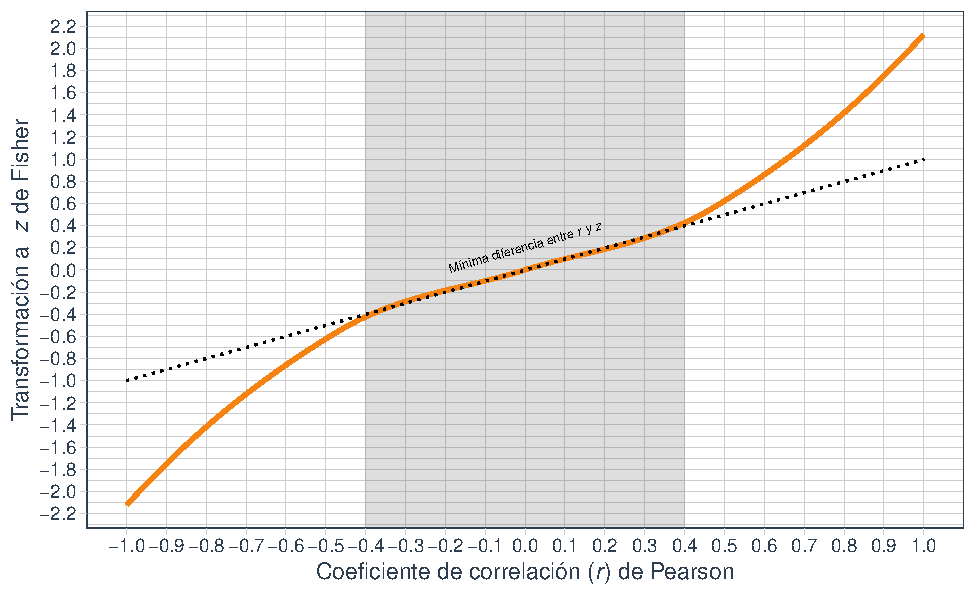
\includegraphics{Meta-analysis_files/figure-latex/rvsz-1.pdf}
\caption{\label{fig:rvsz}Asociación entre coeficientes de correlación \emph{r} de Pearson (eje \emph{X}), y su transformación a \emph{z} de Fisher (eje \emph{Y}). La línea naranja representa la asociación entre valores \emph{r} y \emph{z}; como referencia, la línea negra punteada representa igualdad entre ejes (\emph{y} = \emph{x}). Como se puede ver, cuando \emph{r} está aproximadamente entre -0.4 y 0.4 (rectángulo gris), los valores \emph{r} y \emph{z} son casi idénticos. Para valores más extremos, el valor de \emph{z} se aleja progresivamente del valor de \emph{r}.}
\end{figure}

Por supuesto, si decides reportar los resultados de tu meta-análisis en coeficientes \emph{r} de Pearson, siempre puedes hacer lo mismo con el error estándar y los límites del intervalo de confianza del 95\% (todos valores en \emph{z} de Fisher, pues fue el tamaño de efecto que meta-analizamos).

\hypertarget{muxe1s-informaciuxf3n-sobre-heterogeneidad}{%
\subsection{Más información sobre heterogeneidad}\label{muxe1s-informaciuxf3n-sobre-heterogeneidad}}

Es importante tener en cuenta que la heterogeneidad no es un \emph{supuesto} que se deba cumplir al hacer un meta-análisis, y por ende una heterogeneidad moderada o alta no invalida sus resultados. Sencillamente es información útil que se debe reportar y tener en cuenta al interpretar el resultado de un meta-análisis. En este caso, la presencia de heterogeneidad sugiere que los estudios meta-analizados varían y no suelen reportar resultados similares.

De manera general, y para decirlo de manera más técnica, la presencia de heterogeneidad estadística es indicativa de una variación entre los estudios en la magnitud y la dirección de la estimación del efecto estudiado (para más información y ejemplos, ver \protect\hyperlink{ref-sedgwickMetaanalysesWhatHeterogeneity2015}{Sedgwick, 2015}).

Por esto, reportar información detallada acerca de la heterogeneidad de los estudios meta-analizados es siempre útil. De hecho, además de reportar los estadísticos \(\tau^2\), \(\tau\), \(I^2\) y \(Q\) (como expliqué en la sección \ref{meta-interp}), podemos fácilmente calcular los intervalos de confianza para \(\tau^2\), \(\tau\), e \(I^2\) (además de \(H^2\), que no he usado) con la función \texttt{confint}.

\begin{Shaded}
\begin{Highlighting}[]
\FunctionTok{confint}\NormalTok{(res)}
\end{Highlighting}
\end{Shaded}

\begin{ROut}{Consola de R: Output~\thetcbcounter}
                \begin{footnotesize}
                \begin{verbatim} 
       estimate   ci.lb   ci.ub 
tau^2    0.0081  0.0017  0.0378 
tau      0.0901  0.0412  0.1944 
I^2(%)  61.7324 25.2799 88.2545 
H^2      2.6132  1.3383  8.5139 
 \end{verbatim}
                \end{footnotesize}
                \end{ROut}

Para \(\tau^2\), el hecho de que los límites del intervalo de confianza no crucen el 0 (es decir, no hay un límite negativo y otro positivo; en nuestro caso, ambos son positivos: IC 95\% {[}0.0017, 0.0378{]}), también sugiere que que hay heterogeneidad entre los estudios que meta-analizamos.

Estos intervalos de confianza que también pueden ser reportados junto a sus correspondientes estadísticos. Entonces, esto se podría resumir, por ejemplo, como:

\begin{quote}
El resultado meta-analizado sugiere que en efecto existe una asociación positiva entre concienciación y adherencia a la medicación (\emph{z} ± \emph{se} = 0.15 ± 0.032, IC 95\% {[}0.09, 0.21{]}; \emph{Z} = 4.75, \(p\) \textless{} .0001). Sin embargo, es importante considerar que hay heterogeneidad entre los estudios meta-analizados (\(\tau^2\) ± \emph{se} = 0.0081 ± 0.0055, IC 95\% {[}0.0017, 0.0378{]}; \(\tau\) = 0.0901, IC 95\% {[}0.0412, 0.1944{]}; \(Q\)(15) = 38.16, \(p\) \textless{} .001; \(I^2\) = 61.7\%, IC 95\% {[}25.2799\%, 88.2545\%{]}).
\end{quote}

\hypertarget{diag-inf}{%
\subsection{Diagnóstico de influencia}\label{diag-inf}}

Otro aspecto importante de un meta-análisis, es determinar si alguno(s) de los estudios meta-analizados es(son) particularmente influyente(s) en nuestro resultado\footnote{Por ejemplo, si estuviésemos meta-analizando 20 estudios, de los cuales 19 tienen un \emph{n} de 100, pero el otro tiene un \emph{n} de 10.000, éste último tendrá una influencia enorme en nuestro resultado. Sería preocupante que nuestro meta-análisis sea dependiente principalmente de un único estudio.}. Para esto, se suele usar la técnica conocida como \emph{leave-one-out}, que se refiere al resultado del meta-análisis cuando se excluye cada estudio; al estimar cómo y cuánto cambia el resultado del modelo de meta-análisis al excluir cada estudio, podemos estimar su influencia en el resultado. Dicho de otra manera, si al excluir un estudio el resultado cambia mucho, sabemos que ese estudio tiene gran influencia en el meta-análisis y sería mejor excluirlo.

Para hacer un análisis de influencia, podemos usar la función \texttt{influence} del paquete \texttt{metafor}, cuyo resultado, en este caso, asignaré a un objeto llamado \texttt{inf.res}.

\begin{Shaded}
\begin{Highlighting}[]
\NormalTok{inf.res }\OtherTok{\textless{}{-}} \FunctionTok{influence}\NormalTok{(res)}
\end{Highlighting}
\end{Shaded}

Dado que lo asigné a un objeto (\texttt{inf.res}), para ver el resultado, debo usar como comando el nombre que le di al objeto.

\begin{Shaded}
\begin{Highlighting}[]
\NormalTok{inf.res}
\end{Highlighting}
\end{Shaded}

\begin{ROut}{Consola de R: Output~\thetcbcounter}
                \begin{footnotesize}
                \begin{verbatim} 
   rstudent  dffits cook.d  cov.r tau2.del  QE.del    hat  weight    dfbs inf 
1    0.2918  0.0485 0.0025 1.1331   0.0091 37.7109 0.0568  5.6776  0.0481     
2    0.1196 -0.0031 0.0000 1.2595   0.0100 36.7672 0.1054 10.5396 -0.0032     
3    1.2740  0.2595 0.0660 0.9942   0.0075 35.3930 0.0364  3.6432  0.2623     
4    1.4711  0.3946 0.1439 0.9544   0.0068 33.5886 0.0562  5.6195  0.3994     
5    0.8622  0.1838 0.0339 1.0505   0.0082 36.5396 0.0441  4.4069  0.1837     
6   -0.9795 -0.2121 0.0455 1.0639   0.0084 37.1703 0.0411  4.1094 -0.2112     
7    0.2177  0.0296 0.0010 1.1740   0.0094 37.6797 0.0714  7.1362  0.0296     
8   -0.9774 -0.3120 0.1001 1.1215   0.0084 36.1484 0.0889  8.8886 -0.3128     
9    0.7264  0.1392 0.0195 1.0561   0.0083 37.0495 0.0379  3.7886  0.1387     
10  -1.8667 -0.5861 0.2198 0.8502   0.0047 25.0661 0.1058 10.5826 -0.5430     
11  -1.4985 -0.2771 0.0756 1.0073   0.0077 35.6617 0.0369  3.6922 -0.2791     
12   1.8776  0.4918 0.2148 0.8819   0.0059 31.9021 0.0511  5.1150  0.5059     
13  -1.1892 -0.2939 0.0859 1.0550   0.0080 36.3291 0.0587  5.8732 -0.2941     
14  -0.0020 -0.0423 0.0021 1.2524   0.0100 37.7339 0.0998  9.9778 -0.0434     
15   0.8066  0.2126 0.0459 1.0907   0.0083 35.8385 0.0684  6.8403  0.2125     
16  -0.7160 -0.1656 0.0280 1.0853   0.0087 37.7017 0.0411  4.1094 -0.1642     
 \end{verbatim}
                \end{footnotesize}
                \end{ROut}

Esto me muestra gran cantidad de información de cada estudio (en este caso, lo presento como una tabla sin formato, tal cual se ve en la consola de R). Las columnas que incluye son:

\begin{itemize}
\item
  \texttt{rstudent}: residuo estandarizados externamente. Esto \textbf{no} corresponde al coeficiente de correlación de cada estudio, sino a la diferencia entre el tamaño de efecto observado en cada estudio, y la predicción de dicho valor cuando dicho estudio se elimina del meta-análisis
\item
  \texttt{dffits}: diferencia de ajuste(s) (en inglés \emph{difference in fit(s)}). Es una medida diagnóstica de la influencia de cada punto en una regresión (en este caso, cada estudio en un meta-análisis) propuesta originalmente por Belsley et al. (\protect\hyperlink{ref-belsleyRegressionDiagnosticsIdentifying1980}{1980})
\item
  \texttt{cook.d}: Distancia de Cook (en inglés, \emph{Cook's distance}). Es otra medida diagnóstica de la influencia, propuesta originalmente por Cook (\protect\hyperlink{ref-cookDetectionInfluentialObservation1977}{1977}). Es conceptualmente idéntica a DFFITS (\texttt{dffits}), y he hecho existe una fórmula para convertir una medida en la otra (\protect\hyperlink{ref-Henry2003}{Henry et al., 2003}). Aunque no hay un acuerdo absoluto respecto, comúnmente se asume que valores mayores a 1 (\(D_{i} > 1\)), representan puntos altamente influyentes en un modelo (\protect\hyperlink{ref-cookResidualsInfluenceRegression1982}{Cook \& Weisberg, 1982}), que probablemente deban ser excluidos
\item
  \texttt{cov.r}: relación (o proporción) de covarianza. Es el determinante de la matriz de varianza-covarianza de las estimaciones de los parámetros basadas en el conjunto de datos, cuando cada estudio se elimina del meta-análisis, dividido por el mismo determinante de la matriz de varianza-covarianza cuando se incluyen todos los estudios. Básicamente, un valor menor a 1 indica que la eliminación de ese estudio produce estimaciones más precisas de los coeficientes del modelo
\item
  \texttt{tau2.del}: es la heterogeneidad (residual) \(\tau^2\) cuando se elimina cada estudio
\item
  \texttt{QE.del}: similar al resultado anterior, este se refiere al estadístico \(Q\) obtenido cuando se excluye cada estudio
\item
  \texttt{hat}: los valores \emph{hat} (\(h\)) son una medida estandarizada de la distancia de cada punto a la media de la variable predictora. Mientras valores cercanos a 0 indican que no hay un valor preocupante, valores cercanos a 1, aunque no indican directamente alta influencia de algún punto, ciertamente nos indican que vale la pena investigar más. Los valores \emph{hat} están abiertos a la interpretación, pero un valor de corte que es común es el doble de la media de los todos valores \emph{hat} (\(\overline{h}\)); cualquier estudio con un valor mayor debe ser examinado con cuidado
\item
  \texttt{weight}: peso asignado a cada estudio
\item
  \texttt{dfbs}: el valor de \texttt{dfbs} (o \emph{DFBETAS}) indica cuántas desviaciones estándar cambia el coeficiente estimado después de excluir cada estudio del modelo de meta-análisis
\item
  \texttt{inf}: por suerte, esta columna \texttt{inf} resume esta información por nosotros. Cualquier estudio que se considere influyente, teniendo en cuenta la diferencia de ajuste, la distancia de Cook, los valores \emph{hat} o \emph{DFBETAS}, será señalado acá como influyente, usando asteriscos.
\end{itemize}

Aunque hay mucha información, lo más importante ahora es mirar la última columna, llamada \texttt{inf}. Si ahí aparecieran asteriscos para algún estudio meta-analizado (que no es nuestro caso), sugeriría que ese estudio es particularmente influyente y podría ser necesario eliminarlo del meta-análisis.

Por último, podemos también ver ésta información que tenemos guardada en el objeto \texttt{inf.res}, de manera gráfica, usando la función \texttt{plot} (Fig. \ref{fig:infplot}).

\begin{Shaded}
\begin{Highlighting}[]
\FunctionTok{plot}\NormalTok{(inf.res)}
\end{Highlighting}
\end{Shaded}

\begin{figure}
\centering
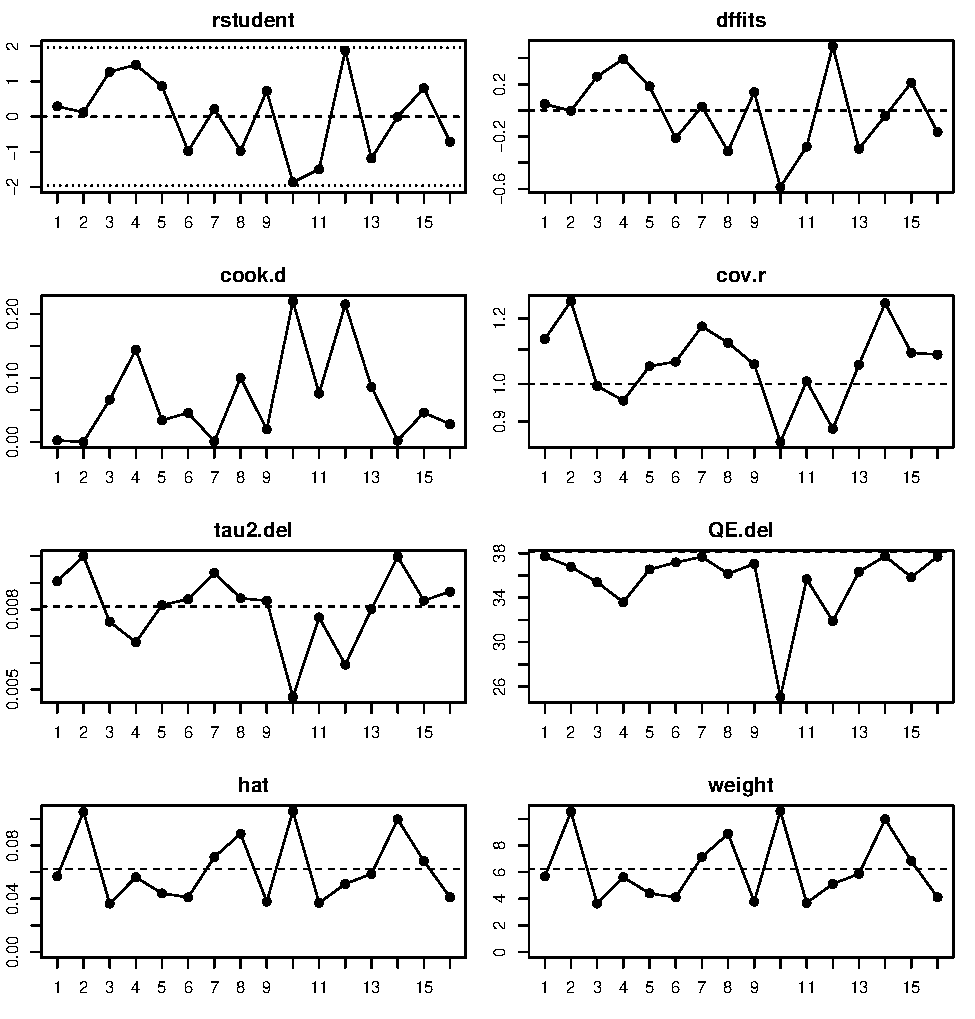
\includegraphics{Meta-analysis_files/figure-latex/infplot-1.pdf}
\caption{\label{fig:infplot}Diagnóstico de influencia. Estudios particularmente influyentes serían representados con un punto rojo. Los números 1 a 16 en el eje \emph{X} representan cada estudio, como lo definimos en columna \texttt{study\_id} de la Tabla \ref{tab:estructuramod}. En este caso, no hay ningún estudio que se considere demasiado influyente, por lo éste análisis sugiere que podemos estar tranquilos con nuestro meta-análisis.}
\end{figure}

\hypertarget{forest-plot-diagrama-de-bosque}{%
\subsection{\texorpdfstring{\emph{Forest plot} (diagrama de bosque)}{Forest plot (diagrama de bosque)}}\label{forest-plot-diagrama-de-bosque}}

Para hacer un diagrama de bosque (\emph{forest plot}) con \href{https://www.metafor-project.org/doku.php}{\texttt{metafor}} resumiendo nuestro meta-análisis, solo tenemos que usar la función \texttt{forest}, usando como argumento el objeto al que asignamos los resultados de nuestro meta-análisis (\texttt{res}; esto produce la Fig. \ref{fig:for-plot1}).

\begin{Shaded}
\begin{Highlighting}[]
\FunctionTok{forest}\NormalTok{(res)}
\end{Highlighting}
\end{Shaded}

\begin{figure}
\centering
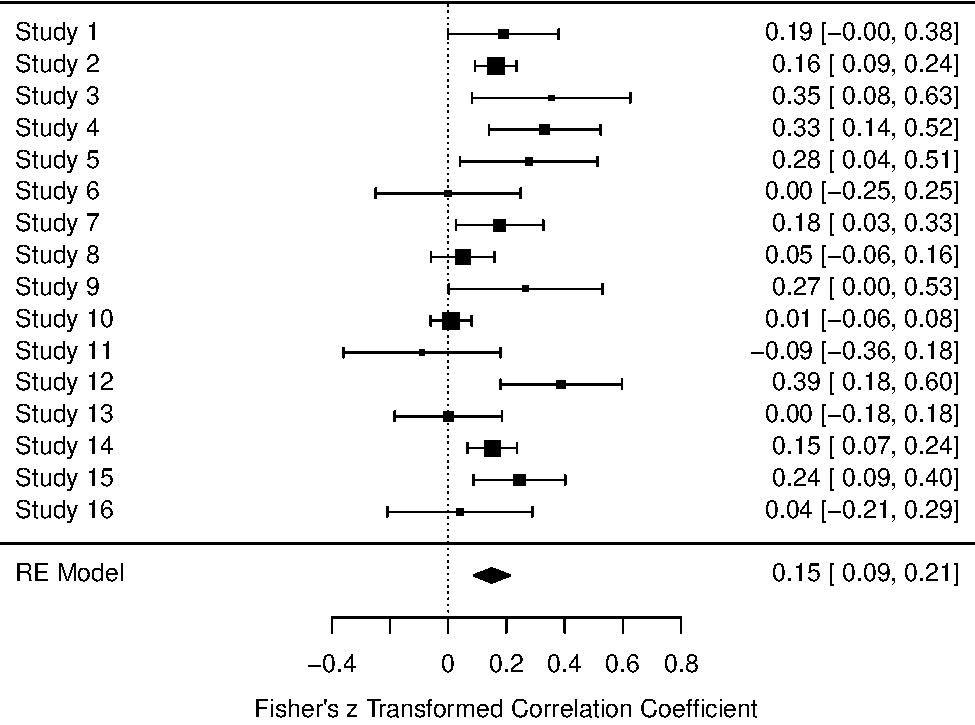
\includegraphics{Meta-analysis_files/figure-latex/for-plot1-1.pdf}
\caption{\label{fig:for-plot1}\emph{Forest plot} básico de \href{https://www.metafor-project.org/doku.php}{metafor}. Para cada estudio meta-analizado, tenemos el efecto (correlación, en este caso en valores \emph{z} de Fisher), así como sus intervalos de confianza entre paréntesis cuadrados. Esta misma información está representada gráficamente, con los cuadrados representando el efecto de cada estudio así como sus intervalos de confianza como barras de error, y el tamaño de muestra representado por el tamaño del cuadrado. Bajo estos resultados, tenemos nuestro meta-análisis, con el mismo formato en texto, pero representando el efecto y sus intervalos de confianza con un diamante.}
\end{figure}

Como se puede ver en las Figuras \ref{fig:for-plot1}, \ref{fig:for-plot2} y \ref{fig:for-plot3b} (que son versiones del mismo \emph{forest plot}), no es una sorpresa que el análisis nos sugiera bastante heterogeneidad; las correlaciones encontradas entre los diferentes estudios varían mucho (están entre -0.09 y 0.37), y aunque son positivas en la mayoría de los casos (en algunos claramente positivas), en otros casos son prácticamente 0 o incluso negativas.

Para una versión más completa y anotada, también usando el \emph{plot} básico de \href{https://www.metafor-project.org/doku.php}{\texttt{metafor}}, pero agregando encabezados de cada columna en español, nombres de los estudios meta-analizados\footnote{En este caso, y dado que tenemos la lista de autores y años de publicación en columnas separadas, pegando las columnas \texttt{authors} y \texttt{year} separadas por una coma y un espacio: \texttt{paste(dat\$authors,\ dat\$year,\ sep\ =\ ",\ ")} como argumento \texttt{slab}.} así como una columna con los pesos dados a cada estudio, y detalles del modelo final\footnote{Estas opciones están explicadas \href{https://search.r-project.org/CRAN/refmans/metafor/html/forest.rma.html}{acá}.}, podemos hacer algo como esto:

\begin{Shaded}
\begin{Highlighting}[]
\CommentTok{\# forest plot con anotaciones adicionales}
\FunctionTok{forest}\NormalTok{(res, }\AttributeTok{cex =} \FloatTok{0.75}\NormalTok{, }\AttributeTok{xlim =} \FunctionTok{c}\NormalTok{(}\SpecialCharTok{{-}}\FloatTok{1.6}\NormalTok{, }\FloatTok{1.6}\NormalTok{),}
       \AttributeTok{slab =} \FunctionTok{paste}\NormalTok{(dat}\SpecialCharTok{$}\NormalTok{authors, dat}\SpecialCharTok{$}\NormalTok{year, }\AttributeTok{sep =} \StringTok{", "}\NormalTok{),}
       \AttributeTok{showweights =} \ConstantTok{TRUE}\NormalTok{,}
       \AttributeTok{xlab =} \StringTok{"Coeficiente de correlación transformado en z de Fisher"}\NormalTok{,}
       \AttributeTok{digits =} \FunctionTok{c}\NormalTok{(}\DecValTok{2}\NormalTok{,3L),}
       \AttributeTok{mlab =} \FunctionTok{bquote}\NormalTok{(}\FunctionTok{paste}\NormalTok{(}\StringTok{"Modelo EA: Q("}\NormalTok{, .(res}\SpecialCharTok{$}\NormalTok{k }\SpecialCharTok{{-}}\NormalTok{ res}\SpecialCharTok{$}\NormalTok{p), }\StringTok{") = "}\NormalTok{,}
\NormalTok{     .(}\FunctionTok{formatC}\NormalTok{(res}\SpecialCharTok{$}\NormalTok{QE, }\AttributeTok{digits =} \DecValTok{2}\NormalTok{, }\AttributeTok{format =} \StringTok{"f"}\NormalTok{)),}
     \StringTok{", p "}\NormalTok{, .(scales}\SpecialCharTok{::}\FunctionTok{pvalue}\NormalTok{(res}\SpecialCharTok{$}\NormalTok{pval)), }\StringTok{"; "}\NormalTok{, I}\SpecialCharTok{\^{}}\DecValTok{2}\NormalTok{, }\StringTok{" = "}\NormalTok{,}
\NormalTok{     .(}\FunctionTok{formatC}\NormalTok{(res}\SpecialCharTok{$}\NormalTok{I2, }\AttributeTok{digits =} \DecValTok{1}\NormalTok{, }\AttributeTok{format =} \StringTok{"f"}\NormalTok{)), }\StringTok{"\%"}\NormalTok{)))}
\CommentTok{\# agregar encabezados a las columnas (valores de X y Y deben ser ajustados)}
\NormalTok{op }\OtherTok{\textless{}{-}} \FunctionTok{par}\NormalTok{(}\AttributeTok{cex =} \FloatTok{0.8}\NormalTok{, }\AttributeTok{font =} \DecValTok{2}\NormalTok{) }
\FunctionTok{text}\NormalTok{(}\AttributeTok{x =} \SpecialCharTok{{-}}\FloatTok{1.6}\NormalTok{, }\AttributeTok{y =} \DecValTok{18}\NormalTok{, }\AttributeTok{labels =} \StringTok{"Autor(es), Año"}\NormalTok{, }\AttributeTok{pos =} \DecValTok{4}\NormalTok{)}
\FunctionTok{text}\NormalTok{(}\AttributeTok{x =} \DecValTok{0}\NormalTok{, }\AttributeTok{y =} \DecValTok{18}\NormalTok{, }\AttributeTok{labels =} \StringTok{"Efecto e IC"}\NormalTok{, }\AttributeTok{pos =} \DecValTok{4}\NormalTok{)}
\FunctionTok{text}\NormalTok{(}\AttributeTok{x =} \DecValTok{1}\NormalTok{, }\AttributeTok{y =} \DecValTok{18}\NormalTok{, }\AttributeTok{labels =} \StringTok{"Peso"}\NormalTok{, }\AttributeTok{pos =} \DecValTok{2}\NormalTok{)}
\FunctionTok{text}\NormalTok{(}\AttributeTok{x =} \FloatTok{1.6}\NormalTok{, }\AttributeTok{y =} \DecValTok{18}\NormalTok{, }\AttributeTok{labels =} \StringTok{"Corr. [95\% IC]"}\NormalTok{, }\AttributeTok{pos =} \DecValTok{2}\NormalTok{)}
\end{Highlighting}
\end{Shaded}

\begin{figure}
\centering
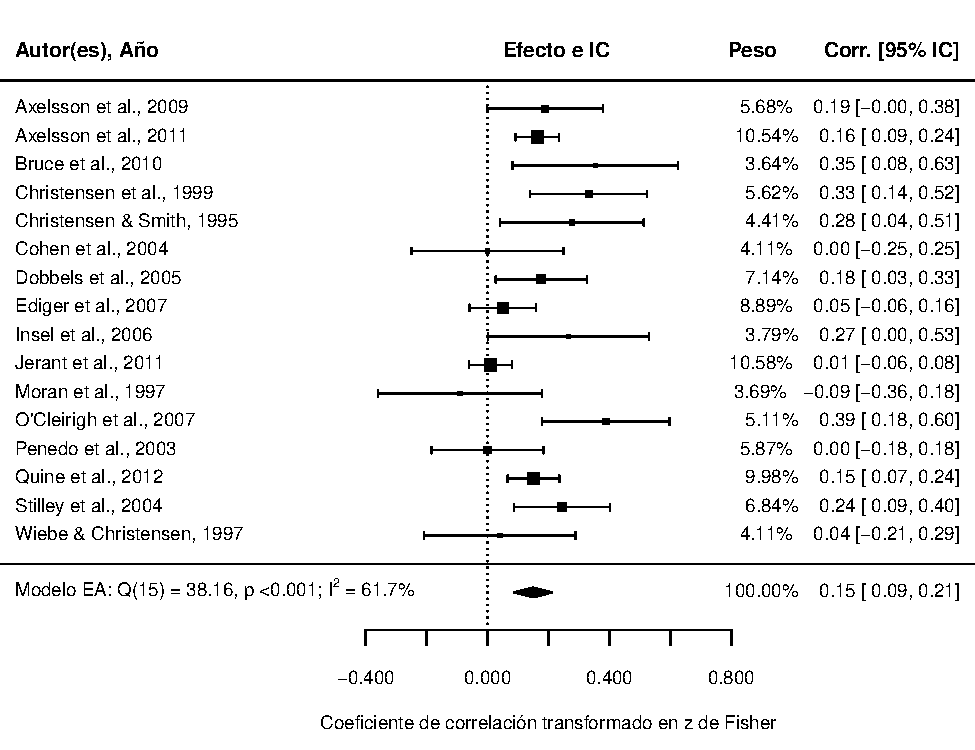
\includegraphics{Meta-analysis_files/figure-latex/for-plot2-1.pdf}
\caption{\label{fig:for-plot2}\emph{Forest plot} anotado, creado con \href{https://www.metafor-project.org/doku.php}{metafor}. En esta versión agregué algunos encabezados en español, así como estadísticos generales del modelo de meta-análisis. Modelo EA se refiere al modelo meta-analizado, de efectos aleatorios.}
\end{figure}

O, para un \emph{forest plot} incluso más sofisticado, se puede usar la función \href{https://cran.r-project.org/web/packages/metaviz/vignettes/metaviz.html\#creating-forest-plots-with-function-viz_forest}{\texttt{viz\_forest}} del paquete \href{https://cran.r-project.org/web/packages/metaviz/vignettes/metaviz.html}{\texttt{metaviz}}.

\begin{Shaded}
\begin{Highlighting}[]
\CommentTok{\# A. Variante "classic" (no tiene que ser definida, pues es la opción por defecto)}
\FunctionTok{viz\_forest}\NormalTok{(res, }
           \AttributeTok{study\_labels =} \FunctionTok{paste}\NormalTok{(dat}\SpecialCharTok{$}\NormalTok{authors, dat}\SpecialCharTok{$}\NormalTok{year, }\AttributeTok{sep =} \StringTok{", "}\NormalTok{),}
           \AttributeTok{xlab =} \StringTok{"Correlación"}\NormalTok{, }
           \AttributeTok{annotate\_CI =} \ConstantTok{TRUE}\NormalTok{,}
           \AttributeTok{summary\_label =} \StringTok{"Resumen"}\NormalTok{,}
           \AttributeTok{text\_size =} \FloatTok{2.6}\NormalTok{,}
           \AttributeTok{x\_trans\_function =}\NormalTok{ tanh)}

\CommentTok{\# B. Variante "thick"}
\FunctionTok{viz\_forest}\NormalTok{(res, }
           \AttributeTok{study\_labels =} \FunctionTok{paste}\NormalTok{(dat}\SpecialCharTok{$}\NormalTok{authors, dat}\SpecialCharTok{$}\NormalTok{year, }\AttributeTok{sep =} \StringTok{", "}\NormalTok{),}
           \AttributeTok{xlab =} \StringTok{"Correlación"}\NormalTok{, }
           \AttributeTok{variant =} \StringTok{"thick"}\NormalTok{,}
           \AttributeTok{col =} \StringTok{"Greens"}\NormalTok{,}
           \AttributeTok{annotate\_CI =} \ConstantTok{TRUE}\NormalTok{,}
           \AttributeTok{summary\_label =} \StringTok{"Resumen"}\NormalTok{,}
           \AttributeTok{text\_size =} \FloatTok{2.6}\NormalTok{,}
           \AttributeTok{x\_trans\_function =}\NormalTok{ tanh)}

\CommentTok{\# C. Variante "rain"}
\FunctionTok{viz\_forest}\NormalTok{(res, }
           \AttributeTok{study\_labels =} \FunctionTok{paste}\NormalTok{(dat}\SpecialCharTok{$}\NormalTok{authors, dat}\SpecialCharTok{$}\NormalTok{year, }\AttributeTok{sep =} \StringTok{", "}\NormalTok{),}
           \AttributeTok{xlab =} \StringTok{"Correlación"}\NormalTok{, }
           \AttributeTok{variant =} \StringTok{"rain"}\NormalTok{,}
           \AttributeTok{col =} \StringTok{"Oranges"}\NormalTok{,}
           \AttributeTok{annotate\_CI =} \ConstantTok{TRUE}\NormalTok{,}
           \AttributeTok{summary\_label =} \StringTok{"Resumen"}\NormalTok{,}
           \AttributeTok{text\_size =} \FloatTok{2.6}\NormalTok{,}
           \AttributeTok{x\_trans\_function =}\NormalTok{ tanh)}
\end{Highlighting}
\end{Shaded}

Con el código anterior genero las siguientes tres versiones del mismo \emph{forest plot} (Fig. \ref{fig:for-plot3b}) usando diferentes variantes y escalas de colores, y transformando de vuelta los coeficientes de \emph{z} de Fisher a \emph{r} de Pearson (con el argumento \texttt{x\_trans\_function\ =\ tanh}).

Por supuesto, es cuestión de gusto cuál usar.

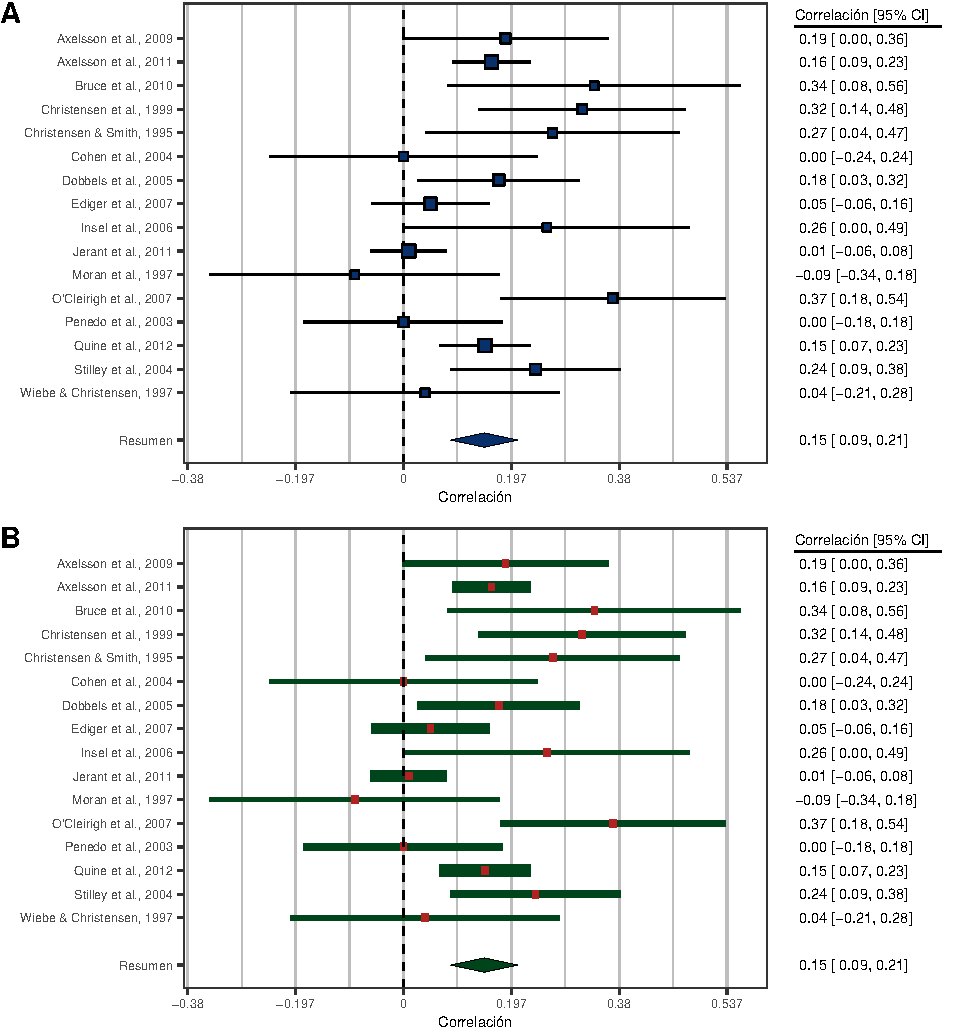
\includegraphics{Meta-analysis_files/figure-latex/for-plot3-1.pdf}

\begin{figure}
\centering
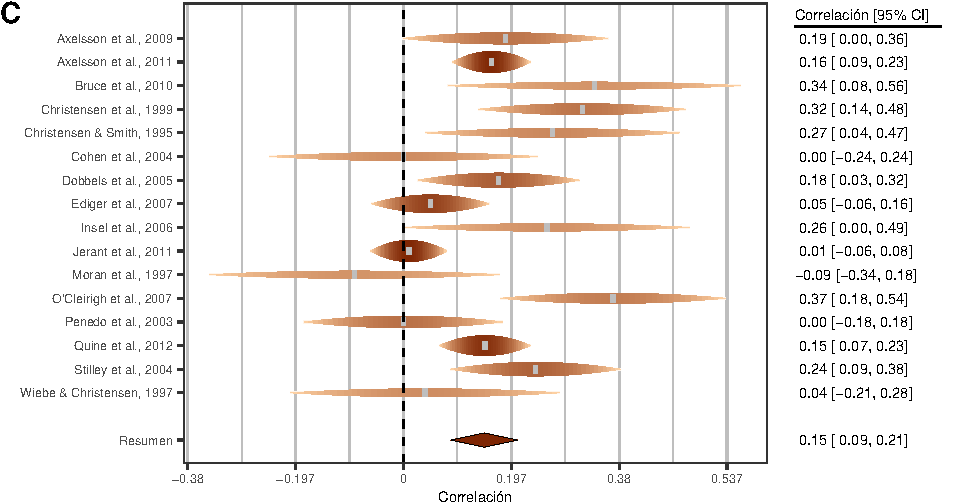
\includegraphics{Meta-analysis_files/figure-latex/for-plot3b-1.pdf}
\caption{\label{fig:for-plot3b}Variantes de \emph{forest plots} creados con \href{https://cran.r-project.org/web/packages/metaviz/vignettes/metaviz.html}{metaviz}. \textbf{A.} Variante clásica (opción por defecto). \textbf{B.} Variante ``thick'' y escala de colores ``Greens''. \textbf{C.} Variante ``rain'' y escala de colores ``Oranges''.}
\end{figure}

\hypertarget{funnel-plot-diagrama-de-embudo-y-sesgo-de-estudios-pequeuxf1os}{%
\subsection{\texorpdfstring{\emph{Funnel plot} (diagrama de embudo) y sesgo de estudios pequeños}{Funnel plot (diagrama de embudo) y sesgo de estudios pequeños}}\label{funnel-plot-diagrama-de-embudo-y-sesgo-de-estudios-pequeuxf1os}}

En este punto, es en donde más errores se cometen. Las pruebas más comunes para evaluar sesgos de publicación, son la evaluación de la asimetría en el \emph{funnel plot} (diagrama de embudo), y la regresión (o test) de Egger (\protect\hyperlink{ref-eggerBiasMetaanalysisDetected1997}{Egger et al., 1997}).

Sin embargo, el principal error que la mayoría de los investigadores (meta-analistas) cometen, es que simplemente basándose en éstos métodos, concluyen que un meta-análisis tiene (o no) riesgo de sufrir de un sesgo de publicación\footnote{Por supuesto, yo mismo soy culpable de haber hecho esto en el pasado, incluyendo algunos comentarios en mi video sobre meta-análisis en \emph{jamovi} (\protect\hyperlink{ref-leongomezMetaanalysis2021}{Leongómez, 2021}).}. Sin embargo, estos métodos, no son pruebas exclusivas de sesgo de publicación, sino de sesgo de estudios de tamaño muestral pequeño (ver e.g. \protect\hyperlink{ref-schwarzerSmallStudyEffectsMetaAnalysis2015}{Schwarzer et al., 2015b}), que pueden incluir sesgo de publicación, pero no se centran exclusivamente en éste.

A pesar de esto, tanto la regresión de Egger como el \emph{funnel plot}, son interesantes dado que el sesgo de estudios pequeños es importante.

\hypertarget{funnel-plot}{%
\subsubsection{\texorpdfstring{\emph{Funnel plot}}{Funnel plot}}\label{funnel-plot}}

Para crear un \emph{funnel plot} con \href{https://www.metafor-project.org/doku.php}{\texttt{metafor}}, de nuestro meta-análisis, solo tenemos que usar la función \texttt{funnel}, usando como argumento el objeto al que asignamos los resultados de nuestro meta-análisis (\texttt{res}). Con esto, generamos la Figura \ref{fig:funnel-plot1}.

\begin{Shaded}
\begin{Highlighting}[]
\FunctionTok{funnel}\NormalTok{(res)}
\end{Highlighting}
\end{Shaded}

\begin{figure}
\centering
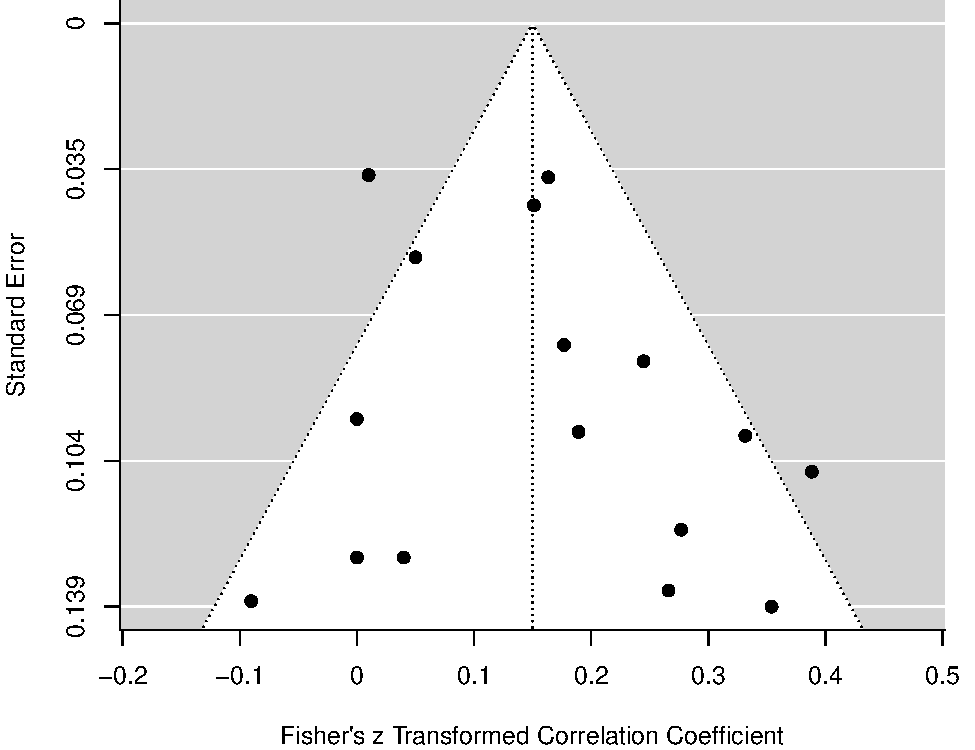
\includegraphics{Meta-analysis_files/figure-latex/funnel-plot1-1.pdf}
\caption{\label{fig:funnel-plot1}\emph{Funnel plot} básico de \href{https://www.metafor-project.org/doku.php}{metafor}. Para cada estudio meta-analizado, tenemos el efecto (correlación, en este caso en valores \emph{z} de Fisher) en el eje \emph{X}, así como su error estándar en el eje \emph{Y}. La línea punteada vertical representa el efecto meta-analizado que hemos encontrado, así que podemos ver los estudios que encontraron un efecto mayor (derecha) o menor (izquierda) que éste. A primera vista no parece haber mucha asimetría, pero es importante tener en cuenta que es un análisis muy subjetivo.}
\end{figure}

O, si queremos cambiar los títulos de los ejes, por ejemplo escribiéndolos en español, podemos hacerlo agregando los argumentos \texttt{xlab} (para el eje \(X\)) y/o \texttt{ylab} (para el eje \(Y\)), como se ve en la Figura \ref{fig:funnel-plot1a}.

\begin{Shaded}
\begin{Highlighting}[]
\FunctionTok{funnel}\NormalTok{(res, }
       \AttributeTok{xlab =} \StringTok{"Coeficiente de correlación transformado en z de Fisher"}\NormalTok{,}
       \AttributeTok{ylab =} \StringTok{"Error estándar"}\NormalTok{)}
\end{Highlighting}
\end{Shaded}

\begin{figure}
\centering
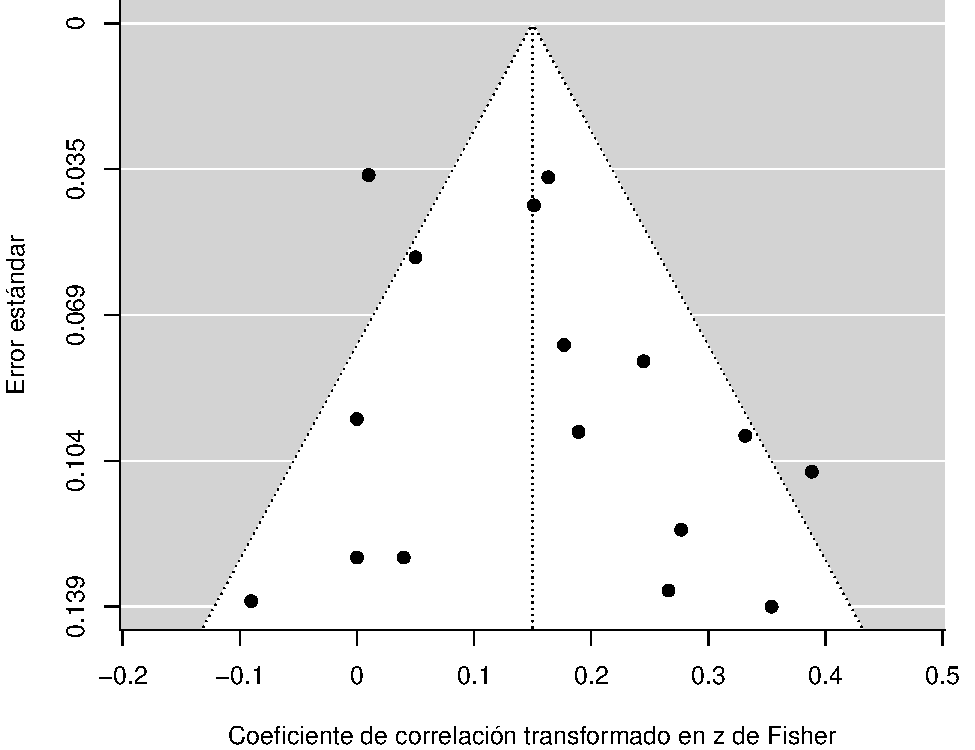
\includegraphics{Meta-analysis_files/figure-latex/funnel-plot1a-1.pdf}
\caption{\label{fig:funnel-plot1a}\emph{Funnel plot} básico de \href{https://www.metafor-project.org/doku.php}{metafor}, con títulos de ejes en español. Para cada estudio meta-analizado, tenemos el efecto (correlación, en este caso en valores \emph{z} de Fisher) en el eje \emph{X}, así como su error estándar en el eje \emph{Y}. La línea punteada vertical representa el efecto meta-analizado que hemos encontrado, así que podemos ver los estudios que encontraron un efecto mayor (derecha) o menor (izquierda) que éste.}
\end{figure}

De nuevo, para una versión más sofisticada, se puede usar el paquete \href{https://cran.r-project.org/web/packages/metaviz/vignettes/metaviz.html}{\texttt{metaviz}}, usando la función \href{https://cran.r-project.org/web/packages/metaviz/vignettes/metaviz.html\#creating-funnel-plots-with-viz_funnel}{\texttt{viz\_funnel}}. Hay muchas opciones, pero como ejemplo, usaré la versión por defecto, agregando solo la línea de la regresión de Egger (\texttt{egger\ =\ TRUE}; ver sección \ref{reg-egger}, más adelante), transformando los tamaños de efecto de regreso a \(r\) de Pearson (\texttt{x\_trans\_function\ =\ tanh}), y con los títulos de los ejes en español (Fig. \ref{fig:funnel-plot2}).

\begin{Shaded}
\begin{Highlighting}[]
\FunctionTok{viz\_funnel}\NormalTok{(res, }
           \AttributeTok{egger =} \ConstantTok{TRUE}\NormalTok{,}
           \AttributeTok{x\_trans\_function =}\NormalTok{ tanh,}
           \AttributeTok{ylab =} \StringTok{"Error estándar"}\NormalTok{,}
           \AttributeTok{xlab =} \StringTok{"Coeficiente de correlación"}\NormalTok{)}
\end{Highlighting}
\end{Shaded}

\begin{figure}
\centering
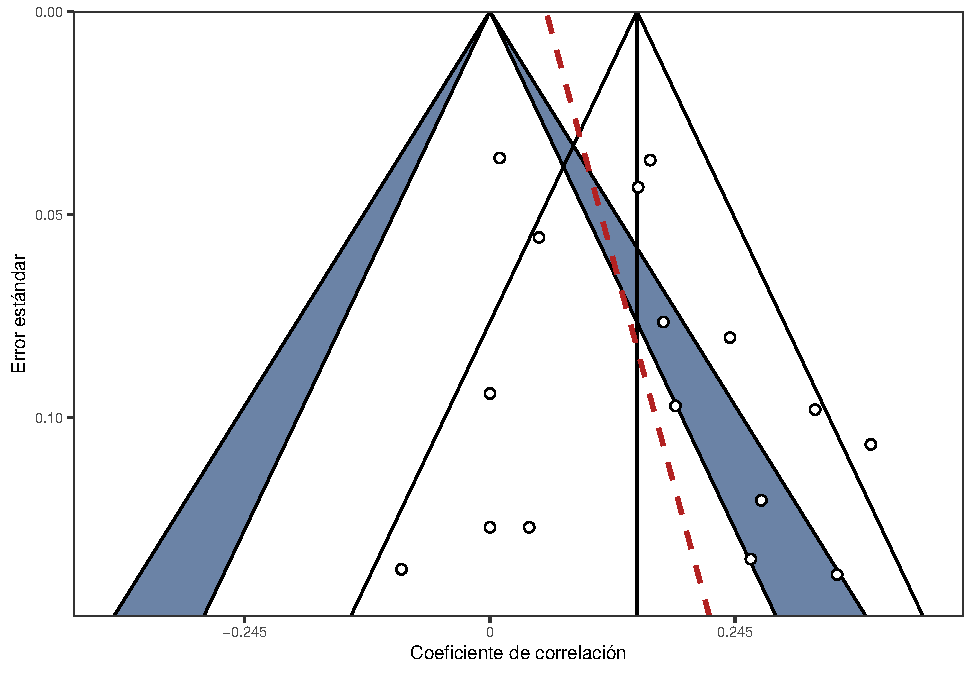
\includegraphics{Meta-analysis_files/figure-latex/funnel-plot2-1.pdf}
\caption{\label{fig:funnel-plot2}\emph{Funnel plot} creado con \href{https://cran.r-project.org/web/packages/metaviz/vignettes/metaviz.html}{metaviz}. En azul, se representa el área donde estudios, según su error (y su tamaño de muestra), tendrían un efecto significativo al 5\% (i.e.~\(p\) \textgreater{} 0.05), y fuera de ésta, donde tendrían un efecto significativo al 1\% (i.e.~\(p\) \textgreater{} 0.01). La línea negra vertical representa el efecto meta-analizado, y el triángulo a partir de su inicio, el área donde se ubican los estudios que no se diferencian significativamente del resultado del meta-análisis. La línea roja punteada, representa la regresión de Egger.}
\end{figure}

Alternativamente, el paquete \href{https://cran.r-project.org/web/packages/metaviz/vignettes/metaviz.html}{\texttt{metaviz}} tiene la función \href{https://cran.r-project.org/web/packages/metaviz/vignettes/metaviz.html\#sunset-power-enhanced-funnel-plots}{\texttt{viz\_sunset}}, que permite además mostrar el poder estadístico (o potencia) de los estudios meta-analizados para detectar un efecto de interés mediante una prueba de Wald de dos colas. De ser necesario, para entender las bases del poder estadístico, recomiendo ver \href{https://youtube.com/playlist?list\%20=\%20PLHk7UNt35ccVdyHqnQ6oXVYA6JBNFrE1x}{esta serie de videos} (\protect\hyperlink{ref-leongomezPoderRvid2020}{Leongómez, 2020b}) y/o, para mayor profundidad, leer \href{https://doi.org/10.5281/zenodo.3988776}{esta guía} (\protect\hyperlink{ref-leongomezAnalisisPoderEstadistico2020}{Leongómez, 2020a}) que publiqué anteriormente.

A continuación, muestro dos versiones de \emph{funnel plots} creados con la función \texttt{viz\_sunset} (Fig. \ref{fig:funnel-plot3}). En ambos casos, agregué el efecto \emph{real} estimado a partir del meta-análisis (\texttt{contours\ =\ TRUE}), y transformé los tamaños de efecto de regreso a \(r\) de Pearson (\texttt{x\_trans\_function\ =\ tanh}).

\begin{Shaded}
\begin{Highlighting}[]
\CommentTok{\# A. Escala de poder discreta}
\FunctionTok{viz\_sunset}\NormalTok{(res,}
           \AttributeTok{contours =} \ConstantTok{TRUE}\NormalTok{,}
           \AttributeTok{x\_trans\_function =}\NormalTok{ tanh)}

\CommentTok{\# B. Escala de poder contínua}
\FunctionTok{viz\_sunset}\NormalTok{(res, }
           \AttributeTok{contours =} \ConstantTok{TRUE}\NormalTok{,}
           \AttributeTok{x\_trans\_function =}\NormalTok{ tanh, }
           \AttributeTok{power\_contours =} \StringTok{"continuous"}\NormalTok{)}
\end{Highlighting}
\end{Shaded}

\begin{figure}
\centering
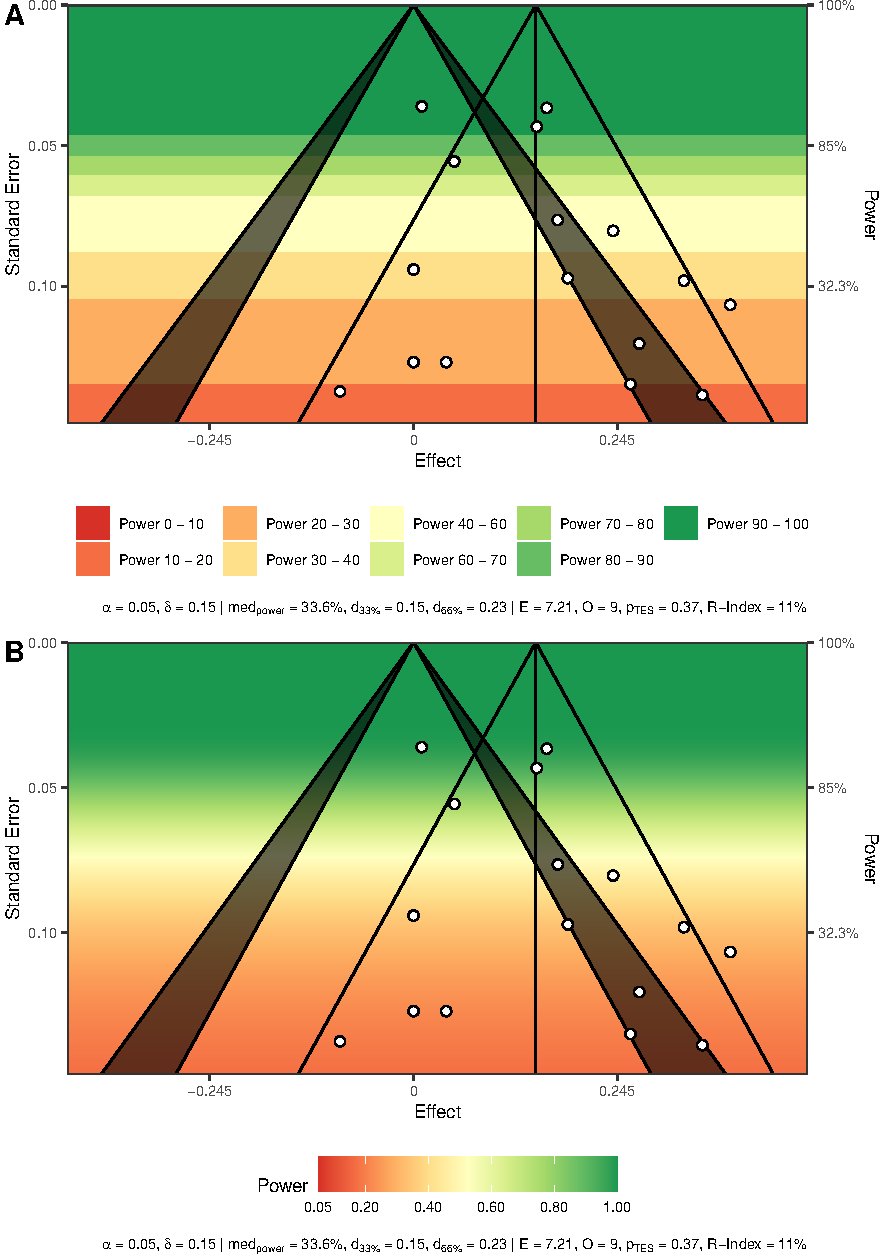
\includegraphics{Meta-analysis_files/figure-latex/funnel-plot3-1.pdf}
\caption{\label{fig:funnel-plot3}Dos versiones de \emph{funnel plot} creados con \href{https://cran.r-project.org/web/packages/metaviz/vignettes/metaviz.html}{metaviz}, usando la función viz-sunset, que estima el poder de cada estudio para detectar un efecto de interés. \textbf{A.} Poder representado por bandas dicretas de color. \textbf{B.} Poder representado de manera contínua en una escala de color. En ambos casos, y tal como en la Fig. \ref{fig:funnel-plot2}, el efecto real está representado como una línea vertical, y el triángulo a partir de su inicio representa el área donde se ubican los estudios que no se diferencian significativamente del resultado del meta-análisis.}
\end{figure}

\hypertarget{reg-egger}{%
\subsubsection{Regresión de Egger}\label{reg-egger}}

Para hacer una prueba formal de sesgo de estudios pequeños (\protect\hyperlink{ref-schwarzerSmallStudyEffectsMetaAnalysis2015}{Schwarzer et al., 2015b}; \protect\hyperlink{ref-sternePublicationRelatedBias2000}{Sterne et al., 2000}), podemos hacer una prueba o regresión de Egger (\protect\hyperlink{ref-eggerBiasMetaanalysisDetected1997}{Egger et al., 1997}). En \href{https://www.metafor-project.org/doku.php}{\texttt{metafor}}, esto se hace con la función \texttt{regtest}, de nuevo usando como argumento el objeto al que asignamos el resultado de nuestro meta-análisis (\texttt{res}).

\begin{Shaded}
\begin{Highlighting}[]
\FunctionTok{regtest}\NormalTok{(res)}
\end{Highlighting}
\end{Shaded}

Como se puede ver, la prueba de Egger no muestra un resultado significativo (\texttt{z\ =\ 1.0216,\ p\ =\ 0.3070}).

\begin{ROut}{Consola de R: Output~\thetcbcounter}
                \begin{footnotesize}
                \begin{verbatim} 
Regression Test for Funnel Plot Asymmetry

Model:     mixed-effects meta-regression model
Predictor: standard error

Test for Funnel Plot Asymmetry: z = 1.0216, p = 0.3070
Limit Estimate (as sei -> 0):   b = 0.0790 (CI: -0.0686, 0.2266)
 \end{verbatim}
                \end{footnotesize}
                \end{ROut}

Con base en esto, y la inspección visual subjetiva del \emph{funnel plot}, muchos investigadores concluyen que no hay sesgo de publicación. Sin embargo, como mencioné antes, estas pruebas no se centran en el sesgo de publicación sino en el sesgo de estudios pequeños. En otras palabras, con base en esto, lo único que podemos concluir correctamente, es que no hay sesgo de estudios pequeños (más adelante, en la sección \ref{sesgo-pub}, explicaré cómo evaluar si hay sesgo de publicación).

\hypertarget{sesgo-pub}{%
\subsection{\texorpdfstring{Sesgo de publicación (\emph{publication bias})}{Sesgo de publicación (publication bias)}}\label{sesgo-pub}}

Existen diferentes opciones para estimar el sesgo de publicación de un meta-análisis. En esta sección, me centraré en dos: el método de recorte y relleno (\emph{trim and fill}), y la estimación del modelo de función de peso.

\hypertarget{trim-fill}{%
\subsubsection{\texorpdfstring{Método \emph{trim and fill} (recorte y relleno)}{Método trim and fill (recorte y relleno)}}\label{trim-fill}}

El método de recorte y relleno (\emph{trim and fill}) es una técnica no paramétrica para aumentar datos (\protect\hyperlink{ref-duvalNonparametricTrimFill2000}{Duval \& Tweedie, 2000a}, \protect\hyperlink{ref-duvalTrimFillSimple2000}{2000b}; ver también \protect\hyperlink{ref-duvalTrimFillMethod2005}{Duval, 2005}). Este método puede utilizarse para estimar y ajustar el número y los resultados de los estudios que faltan en un meta-análisis, con base en el escrutinio de un lado de un diagrama de embudo (\emph{funnel plot}) para estimar la asimetría que se supone que se debe al sesgo de publicación.

Básicamente, el método aumenta los datos observados para que el gráfico de embudo sea más simétrico, y vuelve a calcular la estimación del meta-análisis con base en los datos completos.

Aunque muy útil, es importante tener en cuenta que método de recorte y relleno (\emph{trim and fill}) tiene algunas limitaciones que deben considerarse:

\begin{itemize}
\item
  No debe considerarse como una forma de obtener una estimación más ``válida'' del efecto o resultado global (a partir del meta-análisis), sino como una forma de examinar qué tan sensibles son los resultados a un mecanismo de selección particular (es decir, una forma particular de sesgo de publicación)
\item
  Es importante tener en cuenta que este método no se puede usar en modelos con moderadores, como los que explico en la sección \ref{met-moderation}
\end{itemize}

En \href{https://www.metafor-project.org/doku.php}{\texttt{metafor}}, el método de recorte y relleno (\emph{trim and fill}) se hace simplemente con la función \texttt{trimfill}, de nuevo usando como argumento el objeto al que asignamos el resultado de nuestro meta-análisis (\texttt{res}). En este caso, asignaré el resultado de esta función a un objeto que llamaré \texttt{tf}.

\begin{Shaded}
\begin{Highlighting}[]
\NormalTok{tf }\OtherTok{\textless{}{-}} \FunctionTok{trimfill}\NormalTok{(res)}
\NormalTok{tf}
\end{Highlighting}
\end{Shaded}

\begin{ROut}{Consola de R: Output~\thetcbcounter}
                \begin{footnotesize}
                \begin{verbatim} 
Estimated number of missing studies on the left side: 2 (SE = 2.7118)

Random-Effects Model (k = 18; tau^2 estimator: REML)

tau^2 (estimated amount of total heterogeneity): 0.0112 (SE = 0.0066)
tau (square root of estimated tau^2 value):      0.1061
I^2 (total heterogeneity / total variability):   67.50%
H^2 (total variability / sampling variability):  3.08

Test for Heterogeneity:
Q(df = 17) = 46.3990, p-val = 0.0002

Model Results:

estimate      se    zval    pval   ci.lb   ci.ub      
  0.1288  0.0333  3.8628  0.0001  0.0635  0.1942  *** 

---
Signif. codes:  0 '***' 0.001 '**' 0.01 '*' 0.05 '.' 0.1 ' ' 1
 \end{verbatim}
                \end{footnotesize}
                \end{ROut}

Para crear un \emph{funnel plot} con \href{https://www.metafor-project.org/doku.php}{\texttt{metafor}} del meta-análisis con el método de recorte y relleno (\emph{trim and fill}), solo tenemos que usar la función \texttt{funnel}, usando
como argumento el objeto al que asignamos los resultados del método de recorte y relleno (\texttt{tf}). Con esto, generamos la Figura \ref{fig:tf-plot1}.

\begin{Shaded}
\begin{Highlighting}[]
\FunctionTok{funnel}\NormalTok{(tf, }
       \AttributeTok{xlab =} \StringTok{"Coeficiente de correlación transformado en z de Fisher"}\NormalTok{,}
       \AttributeTok{ylab =} \StringTok{"Error estándar"}\NormalTok{)}
\end{Highlighting}
\end{Shaded}

\begin{figure}
\centering
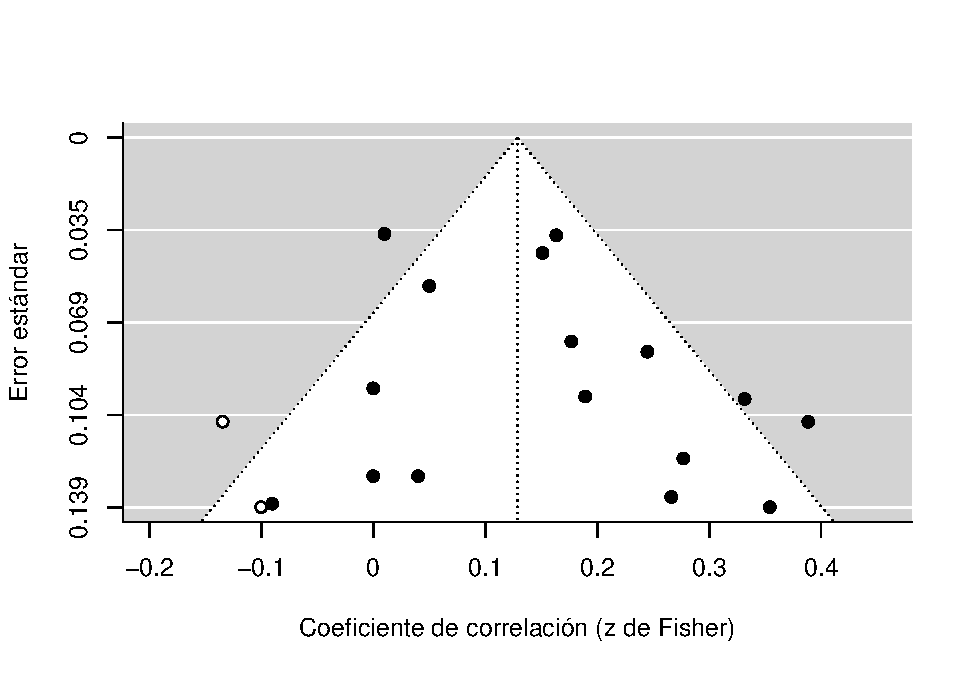
\includegraphics{Meta-analysis_files/figure-latex/tf-plot1-1.pdf}
\caption{\label{fig:tf-plot1}\emph{Funnel plot} básico de \href{https://www.metafor-project.org/doku.php}{metafor} usando el método de recorte y relleno (\emph{trim and fill}). En negro los estudios meta-analizados; en blanco, los estudios \emph{rellenados}.}
\end{figure}

De nuevo, alternativamente podemos usar la función \texttt{viz\_funnel} del paquete \href{https://cran.r-project.org/web/packages/metaviz/vignettes/metaviz.html}{\texttt{metaviz}}, para crear este \emph{funnel plot} representando los estudios \emph{rellenados} con el método de recorte y relleno. Sin embargo, para esto usaremos como argumento el meta-análisis original (\texttt{res}), pero agregando los argumentos \texttt{trim\_and\_fill\ =\ TRUE} y \texttt{trim\_and\_fill\_side\ =\ "left"} (``left'' dado que sabemos que los estudios \emph{faltantes} están a la izquierda del \emph{funnel plot}).

\begin{Shaded}
\begin{Highlighting}[]
\FunctionTok{viz\_funnel}\NormalTok{(res, }
           \AttributeTok{contours\_col =} \StringTok{"Oranges"}\NormalTok{,}
           \AttributeTok{trim\_and\_fill =} \ConstantTok{TRUE}\NormalTok{, }
           \AttributeTok{trim\_and\_fill\_side =} \StringTok{"left"}\NormalTok{, }\CommentTok{\#IMPORTANTE}
           \AttributeTok{egger =} \ConstantTok{TRUE}\NormalTok{,}
           \AttributeTok{x\_trans\_function =}\NormalTok{ tanh,}
           \AttributeTok{ylab =} \StringTok{"Error estándar"}\NormalTok{,}
           \AttributeTok{xlab =} \StringTok{"Coeficiente de correlación"}\NormalTok{) }\SpecialCharTok{+}
  \FunctionTok{geom\_vline}\NormalTok{(}\AttributeTok{xintercept =} \DecValTok{0}\NormalTok{, }\AttributeTok{linetype =} \StringTok{"dotted"}\NormalTok{)}
\end{Highlighting}
\end{Shaded}

\begin{figure}
\centering
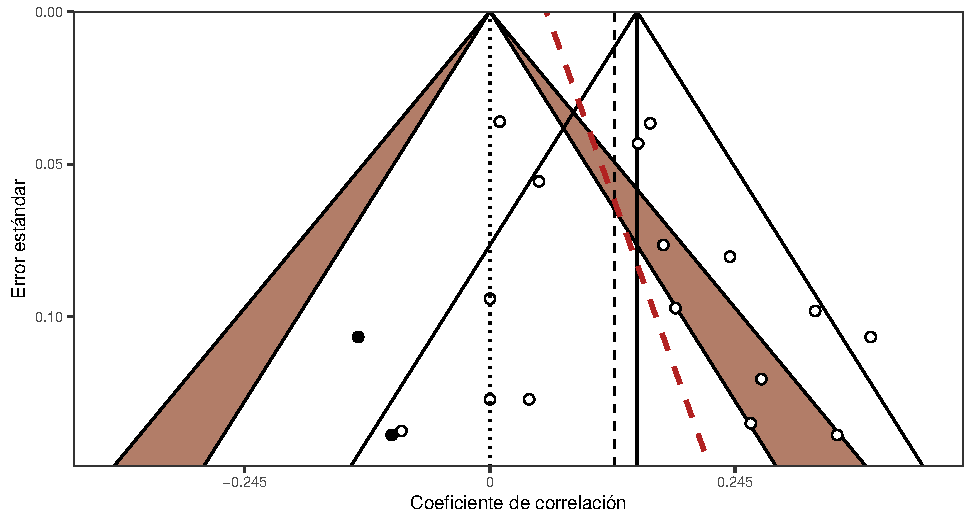
\includegraphics{Meta-analysis_files/figure-latex/tf-plot2-1.pdf}
\caption{\label{fig:tf-plot2}\emph{Funnel plot} creado con \href{https://cran.r-project.org/web/packages/metaviz/vignettes/metaviz.html}{metaviz} usando el método de recorte y relleno (\emph{trim and fill}). En negro los estudios meta-analizados; en blanco, los estudios \emph{rellenados}.}
\end{figure}

El resultado nos muestra que el análisis aumentó dos estudios hipotéticos a la izquierda. Es decir, sugiere que hay \emph{cierto} nivel de sesgo de publicación. De hecho, la estimación del efecto al aumentar estos estudios hipotéticos para que la distribución sea realmente simétrica, disminuye a 0.1288, algo menor que el 0.1499 que nos sugería el análisis inicial.

Si quieres profundizar en el método de recorte y relleno (\emph{trim and fill}), su interpretación, así como sus fortalezas y limitaciones, te recomiendo leer el artículo de Shi \& Lin (\protect\hyperlink{ref-shiTrimandfill2019}{2019}) al respecto.

\hypertarget{estimaciuxf3n-del-modelo-de-funciuxf3n-de-peso}{%
\subsubsection{Estimación del modelo de función de peso}\label{estimaciuxf3n-del-modelo-de-funciuxf3n-de-peso}}

Para determinar el sesgo de publicación, se puede usar la función \texttt{weightfunct} del paquete \texttt{weightr} (\protect\hyperlink{ref-coburnWeightr2019}{Coburn \& Vevea, 2019}), que nos permite ``estimar tanto el modelo de función de peso para el sesgo de publicación que se publicó originalmente en Vevea \& Hedges (\protect\hyperlink{ref-veveaGeneralLinearModel1995}{1995}) como la versión modificada presentada en Vevea \& Woods (\protect\hyperlink{ref-veveaPublicationBiasResearch2005}{2005})'', como se describe en la \href{https://www.rdocumentation.org/packages/weightr/versions/2.0.2/topics/weightfunct}{documentación} de la función \texttt{weightfunct}.

\begin{Shaded}
\begin{Highlighting}[]
\FunctionTok{library}\NormalTok{(weightr)}
\end{Highlighting}
\end{Shaded}

En este caso, usaré esta función, asignando el resultado a un objeto que llamaré \texttt{wf}.

\begin{Shaded}
\begin{Highlighting}[]
\NormalTok{wf }\OtherTok{\textless{}{-}} \FunctionTok{weightfunct}\NormalTok{(}\AttributeTok{effect =}\NormalTok{ dat}\SpecialCharTok{$}\NormalTok{yi, }\AttributeTok{v =}\NormalTok{ dat}\SpecialCharTok{$}\NormalTok{vi, }\AttributeTok{table =} \ConstantTok{TRUE}\NormalTok{)}
\NormalTok{wf}
\end{Highlighting}
\end{Shaded}

\begin{ROut}{Consola de R: Output~\thetcbcounter}
                \begin{footnotesize}
                \begin{verbatim} 
Unadjusted Model (k = 16):

tau^2 (estimated amount of total heterogeneity): 0.0070 (SE = 0.0051)
tau (square root of estimated tau^2 value):  0.0834

Test for Heterogeneity:
Q(df = 15) = 38.1595, p-val = 0.001436053

Model Results:

          estimate std.error z-stat      p-val   ci.lb  ci.ub
Intercept   0.1486   0.03073  4.835 1.3288e-06 0.08837 0.2088

Adjusted Model (k = 16):

tau^2 (estimated amount of total heterogeneity): 0.0056 (SE = 0.0045)
tau (square root of estimated tau^2 value):  0.0750

Test for Heterogeneity:
Q(df = 15) = 38.1595, p-val = 0.001436053

Model Results:

              estimate std.error z-stat    p-val    ci.lb  ci.ub
Intercept      0.09153   0.04464  2.050 0.040341  0.00403 0.1790
0.025 < p < 1  0.24121   0.20122  1.199 0.230626 -0.15317 0.6356

Likelihood Ratio Test:
X^2(df = 1) = 2.98493, p-val = 0.084043

Number of Effect Sizes per Interval:

                     Frequency
p-values <0.025              9
0.025 < p-values < 1         7
 \end{verbatim}
                \end{footnotesize}
                \end{ROut}

El modelo tradicional nos da un estimado muy similar (pero no idéntico) al del estudio original (0.1486), dado que usa un método ligeramente diferente.

Como antes, también nos da valores de heterogeneidad \(\tau^2\), \(\tau\) y \(Q\).

Pero lo más importante, es que nos da los resultado del meta-análisis, ajustando los pesos dados a cada efecto, de cada estudio meta-analizado.

Lo que esta función hace es lo que se conoce como \emph{selection models} (modelos de selección). Básicamente, da más peso a ciertos tamaños de efecto. La realidad de la literatura científica es que es más probable que algunos estudios sean publicados, dependiendo de sus valores \(p\) (\protect\hyperlink{ref-coburnPublicationBiasFunction2015}{Coburn \& Vevea, 2015}; para una descripción sencilla y general, ver por ejemplo \protect\hyperlink{ref-SesgoPublicacion2008}{{``{Acerca del sesgo de publicación en literatura sobre antidepresivos},''} 2008}) publicados que estudios con \(p < 0.05\).

La función \texttt{weightfunct} incrementa el peso de estudios que tienen menos probabilidad de ser publicados, y reduce el peso de estudios con mayor probabilidad de ser publicados. Por esto, al usar ésta técnica, estás asumiendo que de hecho, en el efecto que tratas de encontrar en tu meta-análisis, de hecho hay un sesgo de publicación, lo que a menudo es una suposición bastante justa.

Al usar ésta técnica, tenemos un resultado bastante distinto. Mientras que el meta-análisis original nos daba como resultado un efecto de \textasciitilde0.15, esta técnica nos estima un efecto de \textasciitilde0.09. Básicamente, ha \emph{encogido} nuestro tamaño de efecto.

Al final el \emph{Likelihood ratio test} (algo así como ``Prueba de cociente de probabilidades''), que evalúa la bondad del ajuste de dos modelos estadísticos que compiten entre sí basándose en la relación de su verosimilitud. En este caso, comparando el modelo original, con este modelo con pesos ajustados.

Este resultado nos da una tendencia no descartable (p-val = 0.084043, lo que es \textless{} 0.10; significativa si asumimos un análisis de una cola), que nos da evidencia de que en efecto hay un sesgo de publicación, a pesar de que el \emph{funnel plot} (Figs. \ref{fig:funnel-plot1}, \ref{fig:funnel-plot1a} \ref{fig:funnel-plot2} y \ref{fig:funnel-plot3}) y la regresión de Egger (sección \ref{reg-egger}), sugerían lo contrario.

\hypertarget{poder-estaduxedstico-del-meta-anuxe1lisis}{%
\subsection{Poder estadístico del meta-análisis}\label{poder-estaduxedstico-del-meta-anuxe1lisis}}

En esta sección explicaré cómo hacer un análisis de poder de un meta-análisis; la idea de ésto es saber si nuestro meta-análisis tiene un poder suficiente para detectar el efecto meta-analizado (en nuestro caso 0.15 para el meta-análisis original ``\texttt{res}'', o 0.09 el meta-análisis con pesos ajustados ``\texttt{wf}''). Para este ejemplo, asumiré que el efecto \emph{real} es el encontrado en nuestro análisis original (0.15), pues este efecto es mayor. Si no tuviésemos el poder suficiente para detectar confiablemente ese efecto, menos lo tendríamos para un efecto menor, como el detectado en nuestro meta-análisis con pesos ajustados.

Para hacer esto, usaré el paquete \texttt{metameta} (\protect\hyperlink{ref-quintanaMetameta2022}{Quintana, 2022}, \protect\hyperlink{ref-quintanaGuideMetaPower}{in press}), que permite calcular y visualizar el poder estadístico de un meta-análisis para detectar un rango de posibles efectos \emph{reales}.

\hypertarget{instalaciuxf3n-de-metameta}{%
\subsubsection{\texorpdfstring{Instalación de \texttt{metameta}}{Instalación de metameta}}\label{instalaciuxf3n-de-metameta}}

El paquete \texttt{metameta} se debe instalar desde GitHub\footnote{\href{https://github.com/}{GitHub} es un repositorio abierto para para proyectos de código abierto en el que, entre otras cosas, suelen estar alojados todos los paquetes de R incluso en versiones de desarrollador. Por supuesto, a diferencia de \href{https://cran.r-project.org/}{CRAN}, GitHub es un repositorio de código general, no específico para paquetes de R.} ya que, al día de hoy, no está aún disponible en CRAN.

Para esto, debemos tener instalado el paquete \texttt{devtools}, y usar la función \texttt{install\_github} que nos permite instalar paquetes directamente desde GitHub.

\begin{Shaded}
\begin{Highlighting}[]
\CommentTok{\#se debe tener instalado el paquete devtools}
\FunctionTok{library}\NormalTok{(devtools)}
\FunctionTok{install\_github}\NormalTok{(}\StringTok{"dsquintana/metameta"}\NormalTok{)}
\end{Highlighting}
\end{Shaded}

\hypertarget{anuxe1lisis-de-poder}{%
\subsubsection{Análisis de poder}\label{anuxe1lisis-de-poder}}

Una vez instalado, podemos cargar el paquete.

\begin{Shaded}
\begin{Highlighting}[]
\FunctionTok{library}\NormalTok{(metameta)}
\end{Highlighting}
\end{Shaded}

Como datos, necesitamos no solamente los tamaños de efecto a meta-analizar (\(r\) de Pearson transformado a \emph{z} de Fisher), sino además los intervalos de confianza, tal como fueron reportados en varios de nuestros \emph{Forest plots}.

En este caso, voy a asumir un \emph{efecto real} de \(r = 0.15\), tal como en nuestro meta-análisis original. Sin embargo, el \emph{efecto real} no es algo que podamos saber (es, de hecho, lo que queremos acercarnos a conocer a través del meta-análisis), así que la función \texttt{mapower\_ul} del paquete \texttt{metameta} calcula el poder de cada meta-análisis para un rango de posibles efectos reales.

\begin{Shaded}
\begin{Highlighting}[]
\NormalTok{dat.power }\OtherTok{\textless{}{-}} \FunctionTok{summary}\NormalTok{(dat) }\SpecialCharTok{\%\textgreater{}\%}
  \FunctionTok{select}\NormalTok{(yi, ci.lb, ci.ub) }\SpecialCharTok{\%\textgreater{}\%}
  \FunctionTok{rename}\NormalTok{(}\AttributeTok{lower =}\NormalTok{ ci.lb, }\AttributeTok{upper =}\NormalTok{ ci.ub)}

\NormalTok{power }\OtherTok{\textless{}{-}} \FunctionTok{mapower\_ul}\NormalTok{(}\AttributeTok{dat =}\NormalTok{ dat.power, }\AttributeTok{observed\_es =} \FloatTok{0.15}\NormalTok{, }\AttributeTok{name =} \StringTok{"Molloy et al. 2014"}\NormalTok{)}

\NormalTok{power\_list }\OtherTok{\textless{}{-}} \FunctionTok{list}\NormalTok{(power}\SpecialCharTok{$}\NormalTok{power\_median\_dat)}
\NormalTok{power\_dat }\OtherTok{\textless{}{-}}\NormalTok{ power}\SpecialCharTok{$}\NormalTok{dat}

\NormalTok{power\_list}
\end{Highlighting}
\end{Shaded}

\begin{ROut}{Consola de R: Output~\thetcbcounter}
                \begin{footnotesize}
                \begin{verbatim} [[1]]
  power_es_observed      es01      es02      es03      es04      es05      es06
1                 0 0.1762492 0.5356629 0.8673657 0.9837594 0.9992182 0.9999858
       es07 es08 es09 es1 es_observed meta_analysis_name
1 0.9999999    1    1   1   0.3364197 Molloy et al. 2014
 \end{verbatim}
                \end{footnotesize}
                \end{ROut}

\begin{Shaded}
\begin{Highlighting}[]
\NormalTok{power\_dat}
\end{Highlighting}
\end{Shaded}

\begin{ROut}{Consola de R: Output~\thetcbcounter}
                \begin{footnotesize}
                \begin{verbatim}             yi        lower      upper        sei power_es_observed power_es01
1   0.18922664 -0.001141888 0.37959517 0.09712680         0.3390835  0.1774836
2   0.16343992  0.091680539 0.23519930 0.03661193         0.9837035  0.7797623
3   0.35409253  0.082294427 0.62589063 0.13867250         0.1910727  0.1113715
4   0.33164711  0.139456828 0.52383739 0.09805627         0.3337559  0.1750148
5   0.27686382  0.040911886 0.51281576 0.12038364         0.2383028  0.1320187
6   0.00000000 -0.248915675 0.24891567 0.12699779         0.2188783  0.1234921
7   0.17682002  0.026937828 0.32670221 0.07647051         0.5006730  0.2576556
8   0.05004173 -0.059013584 0.15909704 0.05564047         0.7691106  0.4354589
9   0.26610841  0.001826917 0.53038990 0.13483749         0.1994161  0.1149996
10  0.01000033 -0.060723775 0.08072444 0.03608373         0.9859910  0.7914240
11 -0.09024419 -0.359465946 0.17897757 0.13735804         0.1938536  0.1125800
12  0.38842310  0.179490237 0.59735596 0.10659840         0.2905754  0.1553001
13  0.00000000 -0.184377902 0.18437790 0.09407036         0.3575910  0.1861296
14  0.15114044  0.066324499 0.23595637 0.04327344         0.9340134  0.6371865
15  0.24477411  0.087346017 0.40220221 0.08032046         0.4632371  0.2379950
16  0.04002135 -0.208894321 0.28893703 0.12699779         0.2188783  0.1234921
   power_es02 power_es03 power_es04 power_es05 power_es06 power_es07 power_es08
1   0.5395394  0.8705053  0.9845502  0.9992836  0.9999877  0.9999999  1.0000000
2   0.9997697  1.0000000  1.0000000  1.0000000  1.0000000  1.0000000  1.0000000
3   0.3026621  0.5806100  0.8223954  0.9500825  0.9910281  0.9989921  0.9999302
4   0.5317864  0.8642261  0.9829686  0.9991528  0.9999840  0.9999999  1.0000000
5   0.3827659  0.7026651  0.9135189  0.9858616  0.9987531  0.9999421  0.9999986
6   0.3502733  0.6562694  0.8829174  0.9759855  0.9971497  0.9998088  0.9999929
7   0.7439048  0.9751837  0.9994638  0.9999977  1.0000000  1.0000000  1.0000000
8   0.9489275  0.9997002  0.9999999  1.0000000  1.0000000  1.0000000  1.0000000
9   0.3170763  0.6044851  0.8429297  0.9597856  0.9936099  0.9993842  0.9999645
10  0.9998300  1.0000000  1.0000000  1.0000000  1.0000000  1.0000000  1.0000000
11  0.3074782  0.5886809  0.8294859  0.9535367  0.9919839  0.9991443  0.9999443
12  0.4666848  0.8035418  0.9634686  0.9968384  0.9998781  0.9999980  1.0000000
13  0.5659845  0.8904902  0.9890522  0.9996035  0.9999950  1.0000000  1.0000000
14  0.9961139  0.9999997  1.0000000  1.0000000  1.0000000  1.0000000  1.0000000
15  0.7019697  0.9620572  0.9987365  0.9999900  1.0000000  1.0000000  1.0000000
16  0.3502733  0.6562694  0.8829174  0.9759855  0.9971497  0.9998088  0.9999929
   power_es09 power_es1
1   1.0000000 1.0000000
2   1.0000000 1.0000000
3   0.9999971 0.9999999
4   1.0000000 1.0000000
5   1.0000000 1.0000000
6   0.9999999 1.0000000
7   1.0000000 1.0000000
8   1.0000000 1.0000000
9   0.9999988 1.0000000
10  1.0000000 1.0000000
11  0.9999978 0.9999999
12  1.0000000 1.0000000
13  1.0000000 1.0000000
14  1.0000000 1.0000000
15  1.0000000 1.0000000
16  0.9999999 1.0000000
 \end{verbatim}
                \end{footnotesize}
                \end{ROut}

\hypertarget{visualizaciuxf3n-del-anuxe1lisis-de-poder-firepower-plot}{%
\subsubsection{\texorpdfstring{Visualización del análisis de poder (\emph{Firepower plot})}{Visualización del análisis de poder (Firepower plot)}}\label{visualizaciuxf3n-del-anuxe1lisis-de-poder-firepower-plot}}

Según esto, nuestro meta-análisis solo tiene un poder estadístico suficiente para detectar de manera confiable efectos mayores a \textasciitilde0.3, lo que está muy por encima de nuestras estimaciones del efecto real (0.15 en nuestro meta-análisis original, 0.09 en nuestro meta-análisis con pesos ajustados).

\begin{Shaded}
\begin{Highlighting}[]
\NormalTok{power.plot }\OtherTok{\textless{}{-}} \FunctionTok{firepower}\NormalTok{(power\_list)}
\end{Highlighting}
\end{Shaded}

Para ver el \emph{fireplot} que creamos, y ya que lo asigné a un objeto que llamé \texttt{power.plot}, debo correr el objeto para ver el resultado (Fig. \ref{fig:fire-plot1}).

\begin{Shaded}
\begin{Highlighting}[]
\NormalTok{power.plot}
\end{Highlighting}
\end{Shaded}

\begin{figure}
\centering
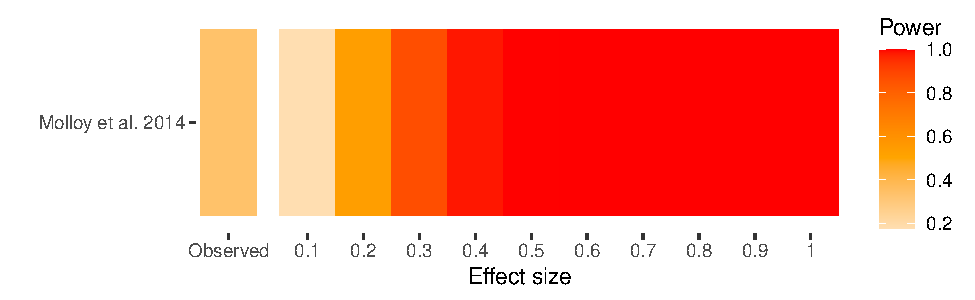
\includegraphics{Meta-analysis_files/figure-latex/fire-plot1-1.pdf}
\caption{\label{fig:fire-plot1}Fireplot básico de \href{https://www.dsquintana.blog/metameta-r-package-meta-analysis/}{metameta}, para un análisis de poder de nuestro meta-análisis. \emph{Observed} hace referencia al tamaño de efecto observado en nuestro meta-análisis original; en este caso, 0.15.}
\end{figure}

Si queremos cambiar los títulos a español, y ya que el objeto \texttt{power.plot} contiene dos elementos (\texttt{dat} y \texttt{fp\_plot}, que es propiamente la gráfica). Éste último elemento es de clase \texttt{ggplot}, por lo que podemos usar funciones de \texttt{ggplot2} para cambiar, por ejemplo, el título del eje \(X\) a ``Tamaño de efecto'', el título de la leyenda a ``Poder'', y el efecto observado de ``\emph{Observed}'' a ``Observado''\footnote{Para cambiar el título del eje \(X\) usé la función \texttt{xlab}; para el título de la leyenda la función \texttt{guides} (opción \texttt{fill\ =\ guide\_legend}); y para los valores del eje \(X\), la función \texttt{scale\_x\_discrete}\}.} (Fig. \ref{fig:fire-plot2}). Por ejemplo:

\begin{Shaded}
\begin{Highlighting}[]
\NormalTok{power.plot}\SpecialCharTok{$}\NormalTok{fp\_plot }\SpecialCharTok{+}
  \FunctionTok{xlab}\NormalTok{(}\StringTok{"Tamaño de efecto"}\NormalTok{) }\SpecialCharTok{+}
  \FunctionTok{guides}\NormalTok{(}\AttributeTok{fill =} \FunctionTok{guide\_legend}\NormalTok{(}\AttributeTok{title =} \StringTok{"Poder"}\NormalTok{, }
                             \AttributeTok{reverse =} \ConstantTok{TRUE}\NormalTok{)) }\SpecialCharTok{+}
  \FunctionTok{scale\_x\_discrete}\NormalTok{(}\AttributeTok{labels =} \FunctionTok{c}\NormalTok{(}\StringTok{"es\_observed"} \OtherTok{=} \StringTok{"Observado"}\NormalTok{,}
                              \StringTok{"es01"} \OtherTok{=} \FloatTok{0.1}\NormalTok{,    }
                              \StringTok{"es02"} \OtherTok{=} \FloatTok{0.2}\NormalTok{,}
                              \StringTok{"es03"} \OtherTok{=} \FloatTok{0.3}\NormalTok{,}
                              \StringTok{"es04"} \OtherTok{=} \FloatTok{0.4}\NormalTok{,    }
                              \StringTok{"es05"} \OtherTok{=} \FloatTok{0.5}\NormalTok{,    }
                              \StringTok{"es06"} \OtherTok{=} \FloatTok{0.6}\NormalTok{,    }
                              \StringTok{"es07"} \OtherTok{=} \FloatTok{0.7}\NormalTok{,}
                              \StringTok{"es08"} \OtherTok{=} \FloatTok{0.8}\NormalTok{,}
                              \StringTok{"es09"} \OtherTok{=} \FloatTok{0.9}\NormalTok{,}
                              \StringTok{"es1"}  \OtherTok{=} \DecValTok{1}\NormalTok{))}
\end{Highlighting}
\end{Shaded}

\begin{figure}
\centering
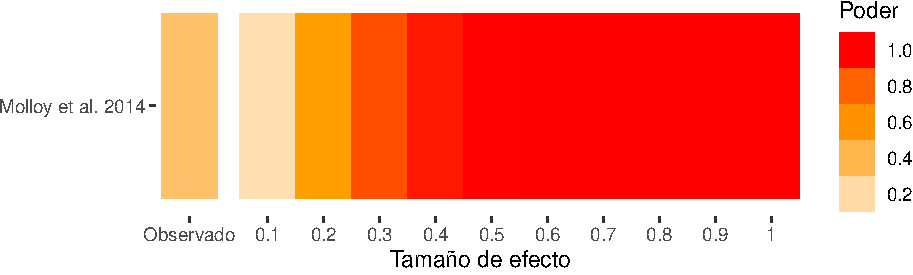
\includegraphics{Meta-analysis_files/figure-latex/fire-plot2-1.pdf}
\caption{\label{fig:fire-plot2}Fireplot básico de \href{https://www.dsquintana.blog/metameta-r-package-meta-analysis/}{metameta}, para un análisis de poder de nuestro meta-análisis, con el texto traducido a español y con la leyenda en una escala discreta para facilitar su lectura. \emph{Observado} hace referencia al tamaño de efecto observado en nuestro meta-análisis original (en este caso, 0.15).}
\end{figure}

\hypertarget{analizar-todas-las-posibles-combinaciones-de-estudios}{%
\subsection{Analizar todas las posibles combinaciones de estudios}\label{analizar-todas-las-posibles-combinaciones-de-estudios}}

Ver acá \url{https://www.dsquintana.blog/combinatorial-meta-analysis/}

\hypertarget{leave-one-out}{%
\subsubsection{\texorpdfstring{\emph{Leave-one-out}}{Leave-one-out}}\label{leave-one-out}}

La técnica de \emph{leave-one-out} no solo se puede hacer como parte de un diagnóstico de influencia (como se muestra en la sección \ref{diag-inf}), sino que también se puede hacer para ver la estimación del efecto meta-analizado al excluir cada uno de los estudios de nuestra base de datos.

Hacerlo solo requiere usar la función \texttt{leave1out} del paquete \texttt{metafor}, usando como argumento el resultado de nuestro meta-análisis original (en este caso, \texttt{res}):

\begin{Shaded}
\begin{Highlighting}[]
\FunctionTok{leave1out}\NormalTok{(res)}
\end{Highlighting}
\end{Shaded}

Como puedes ver, nos crea una tabla con las columnas \texttt{estimate}, \texttt{se}, \texttt{zval}, \texttt{pval}, \texttt{ci.lb}, \texttt{ci.ub}, \texttt{Q}, \texttt{Qp}, \texttt{tau2}, \texttt{I2} y \texttt{H2} (explicadas en la sección \ref{meta-interp}). Sin embargo, tenemos 16 filas, cada una de las cuales corresponde a los resultados cuando se excluye cada estudio del meta-análisis.

\hypertarget{meta-anuxe1lisis-combinatorio}{%
\subsubsection{Meta-análisis combinatorio}\label{meta-anuxe1lisis-combinatorio}}

Aunque la técnica de \emph{leave-one-out} es útil para determinar la influencia de cada estudio en un meta-análisis (como se explica en las secciones \ref{diag-inf} y \ref{leave-one-out}), tiene limitaciones, pues no nos dice nada de cuánto cambia la estimación del efecto meta-analizado cuando excluimos 2 o más estudios. XXXXXXXXX SIGO ACÁ XXXXXXX

\textbf{EXPLICAR LAS VENTAJAS DE HACER TODAS LAS COMBINACIONES POSIBLES}

El número de análisis a realizar puede calcularse usando la fórmula \(2^k - 1\), donde \(k\) es el número de estudios meta-analizados. Como en nuestro ejemplo estamos meta-analizando 16 estudios, realizarás \(2^{16} - 1\) análisis. Es decir, un total de 65535 modelos. Ten en cuenta que ajustar estos 65535 podría bastante tiempo (en mi portátil, que tiene un procesador Intel Core i7-9750H, tardó poco más de 5 minutos, pero puede variar mucho según las características de tu equipo).

Para visualizar esta enorme cantidad de estimaciones de tamaño de efecto, lo mejor es hacer un \emph{visualización gráfica de la heterogeneidad de los estudios} (en inglés, \emph{Graphical Display of Study Heterogeneity} o simplemente \emph{GOSH}), una técnica propuesta por Olkin et al. (\protect\hyperlink{ref-olkinGOSHGraphicalDisplay2012}{2012}).

En R, esto se puede hacer con la función \texttt{gosh} del paquete \texttt{metafor}, agregando como único argumento el resultado de nuestro meta-análisis original (en nuestro caso, \texttt{res}). Voy a asignar el resultado de este análisis a un objeto que llamaré \texttt{gp}

\begin{Shaded}
\begin{Highlighting}[]
\NormalTok{gp }\OtherTok{\textless{}{-}} \FunctionTok{gosh}\NormalTok{(res)}
\end{Highlighting}
\end{Shaded}

\begin{verbatim}
Fitting 65535 models (based on all possible subsets).
\end{verbatim}

Para graficar los los 65535 modelos, podemos usar la función \texttt{plot}, agregando como argumento el resultado de la función \texttt{gosh}(\texttt{gp} en este caso). En este ejemplo, adicionalmente, usaré el argumento \texttt{breaks} para definir el número de puntos de corte (y número de barras) de los histogramas, así como el argumento \texttt{labels} para poner los títulos de los ejes en español.

\begin{Shaded}
\begin{Highlighting}[]
\FunctionTok{plot}\NormalTok{(gp, }
     \AttributeTok{breaks =} \DecValTok{100}\NormalTok{,}
     \AttributeTok{labels =} \FunctionTok{c}\NormalTok{(}\StringTok{"Coeficiente de correlación transformado en z de Fisher"}\NormalTok{, }
                \FunctionTok{expression}\NormalTok{(}\FunctionTok{paste}\NormalTok{(}\StringTok{"I"}\SpecialCharTok{\^{}}\StringTok{"2"}\NormalTok{))))}
\end{Highlighting}
\end{Shaded}

\begin{figure}
\centering
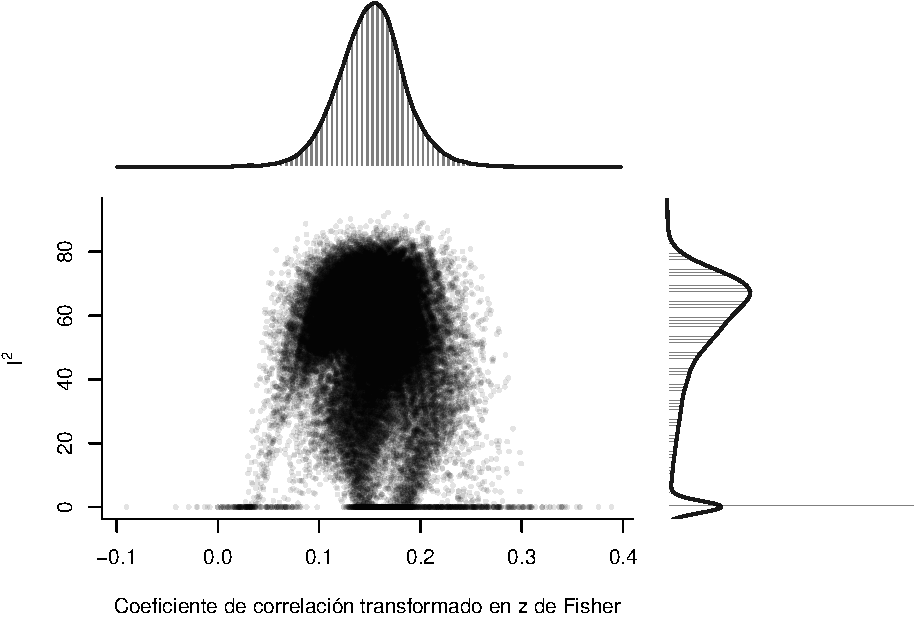
\includegraphics{Meta-analysis_files/figure-latex/gosh1-1.pdf}
\caption{\label{fig:gosh1}\emph{GOSH plot} creado con la función \href{https://www.metafor-project.org/doku.php/plots:gosh_plot}{\texttt{gosh}} del paquete \href{https://www.metafor-project.org/doku.php}{\texttt{metafor}}. Un \emph{GOSH plot} (en inglés, \emph{Graphical Display of Study Heterogeneity} o simplemente \emph{GOSH}) es una visualización gráfica de la heterogeneidad de todos los posibles modelos de meta-análisis ajustados a partir de todas las combinaciones posibles de estudios de nuestra base de datos. Un \emph{GOSH plot} muestra los efectos estimados para cada uno de los modelos en el eje horizontal, y su respectiva heterogeneidad en el eje vertical. Las distribuciones de los efectos (parte superior de la gráfica) y las heterogeneidades (lado derecho de la gráfica) estan representadas como densidades e histogramas.}
\end{figure}

Como puedes ver, los tamaños del efecto suelen estar entre aproximadamente 0.05 y 0.25. Esto es una variación muy grande, que demuestra cómo la elección de los estudios incluidos influye en la estimación del tamaño del efecto que nos dará nuestro meta-análisis.

Para ilustrar mejor esto, podemos a cambiar artificialmente nuestra base de datos, para que contengo valores atípicos.

Para hacer esto, voy a agregar valores atípicos, cambiando manualmente el tamaño de efecto de 2 de los estudios (en este caso, los estudios 12 y 15, que pasan de tener valores \emph{z} de Fisher de 0.39 y 0.24, a otro mayores, de 0.7 y 0.6, respectivamente). Esta base de datos alterada por supuesto ya no tendía validez para realizar ningún análisis, pues 2 de nuestros resultados son literalmente inventados. Sin embargo, nos permite ver qué sucede cuando una base de datos contiene valores atípicos.

Dado que no quiero afectar nuestra base de datos (\texttt{dat}), voy a crear una copia en un objeto llamado \texttt{dat\_mo}, y después sí cambiar los tamaños de efecto de los estudios 12 y 15 de esa base de datos.

\begin{Shaded}
\begin{Highlighting}[]
\NormalTok{dat\_mo }\OtherTok{\textless{}{-}}\NormalTok{ dat}
\NormalTok{dat\_mo}\SpecialCharTok{$}\NormalTok{yi[}\DecValTok{12}\NormalTok{] }\OtherTok{=} \FloatTok{0.7} 
\NormalTok{dat\_mo}\SpecialCharTok{$}\NormalTok{yi[}\DecValTok{15}\NormalTok{] }\OtherTok{=} \FloatTok{0.6} 
\end{Highlighting}
\end{Shaded}

Voy a hacer un meta-análisis de esta nueva base de datos alterada (\texttt{dat\_mo}), y representar los resultados en un \emph{forest plot} (diagrama de bosque).

\begin{Shaded}
\begin{Highlighting}[]
\NormalTok{res\_mo }\OtherTok{\textless{}{-}} \FunctionTok{rma.uni}\NormalTok{(yi, vi, }\AttributeTok{data =}\NormalTok{ dat\_mo) }
\FunctionTok{forest}\NormalTok{(res\_mo)}
\end{Highlighting}
\end{Shaded}

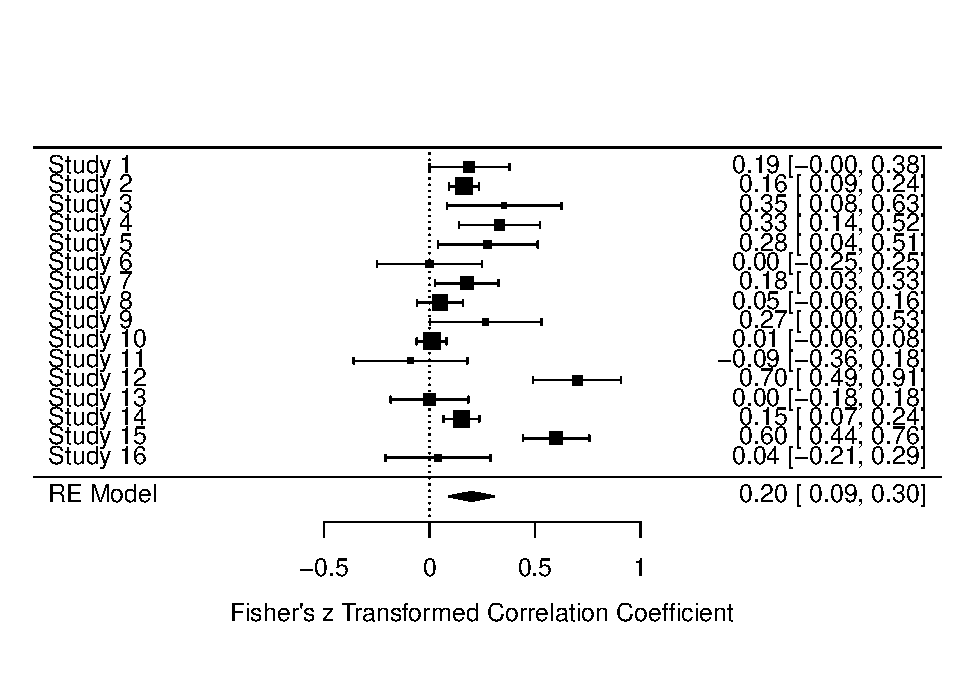
\includegraphics{Meta-analysis_files/figure-latex/unnamed-chunk-31-1.pdf}

Los valores atípicos introducidos son claramente visibles en el \emph{forest plot} (diagrama de bosque). (estudios 12 y 15).

Now let's run the combinatorial meta-analysis and create a GOSH plot:

\begin{Shaded}
\begin{Highlighting}[]
\NormalTok{gp\_mo }\OtherTok{\textless{}{-}} \FunctionTok{gosh}\NormalTok{(res\_mo)}
\end{Highlighting}
\end{Shaded}

\begin{verbatim}
Fitting 65535 models (based on all possible subsets).
\end{verbatim}

Y el plot

\begin{Shaded}
\begin{Highlighting}[]
\FunctionTok{plot}\NormalTok{(gp\_mo, }\AttributeTok{breaks =} \DecValTok{100}\NormalTok{)}
\end{Highlighting}
\end{Shaded}

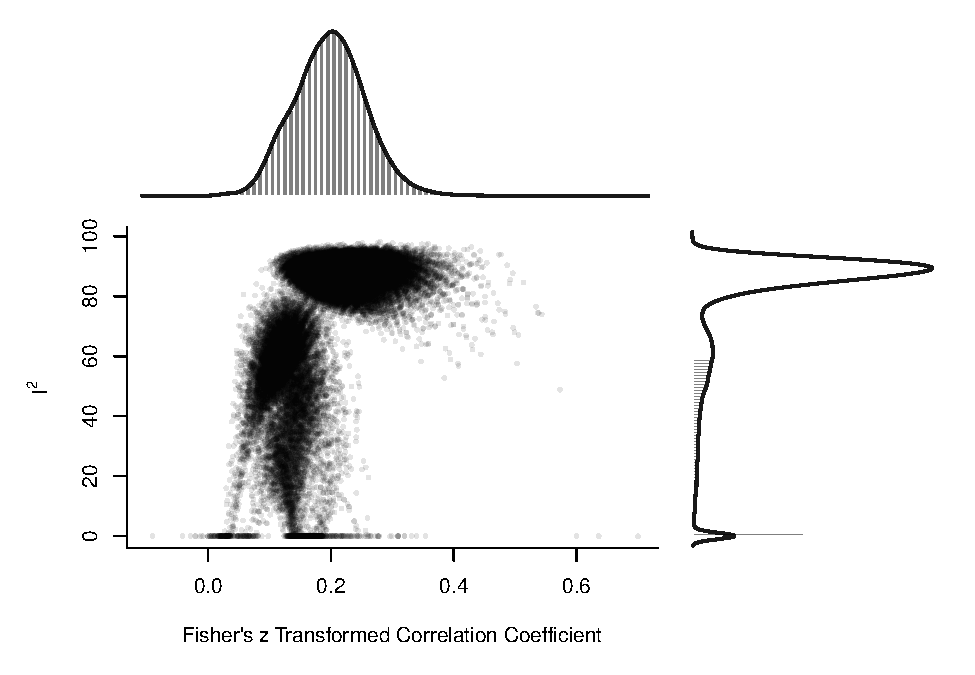
\includegraphics{Meta-analysis_files/figure-latex/unnamed-chunk-33-1.pdf}

There is a clear cluster of large effect sizes with high heterogeneity in the top right of the plot. We can specifically highlight the meta-analysis models that included the potential outlier studies:

\begin{Shaded}
\begin{Highlighting}[]
\FunctionTok{plot}\NormalTok{(gp\_mo, }\AttributeTok{out =} \DecValTok{12}\NormalTok{, }\AttributeTok{breaks =} \DecValTok{100}\NormalTok{,}
     \AttributeTok{labels =} \FunctionTok{c}\NormalTok{(}\StringTok{"Coeficiente de correlación transformado en z de Fisher"}\NormalTok{, }
                \FunctionTok{expression}\NormalTok{(}\FunctionTok{paste}\NormalTok{(}\StringTok{"I"}\SpecialCharTok{\^{}}\StringTok{"2"}\NormalTok{))))}
\end{Highlighting}
\end{Shaded}

\begin{figure}
\centering
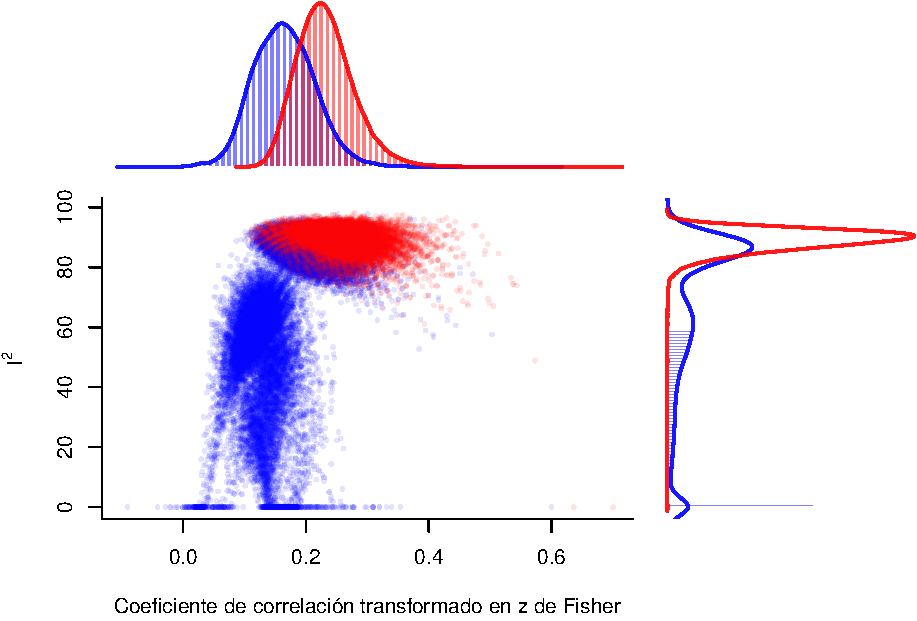
\includegraphics{Meta-analysis_files/figure-latex/unnamed-chunk-34-1.pdf}
\caption{\label{fig:unnamed-chunk-34}Se puede ver en las distribuciones del eje X (distribuciones arriba) cómo los meta análisis que incluyen ese estudio tienden a arrojar estimados más fuertes para la asociación, sesgando el resultado hacia valores más extremos.}
\end{figure}

There's a noticeable shift in the distribution of meta-analysis model summary effect size estimates that include study 12.

Ultimately, combinatorial meta-analysis paired with GOSH plots demonstrate how your analysis choices influence your meta-analysis outcomes and conclusions.

\hypertarget{met-moderation}{%
\section{Meta-análisis de correlación con moderador (meta-regresión)}\label{met-moderation}}

\textcolor{red}{Incluir moderadores en nuestro meta-análisis (i.e. hacer una meta-regresión), es una fusión de principios de regresión meta-analíticos y lineales, que sirva para explorar la heterogeneidad. Con esto, podemos saber si existe una asociación lineal entre el resultado de nuestro meta-análisis y una o más covariables.}

\textcolor{red}{La meta-regresión desempeña un papel fundamental en la consideración de los efectos de las covariables, especialmente en presencia de variables categóricas que pueden utilizarse para el análisis de subgrupos.}

\hypertarget{ex.mod1}{%
\subsection{Ejemplo 1: Moderación de una variable continua (edad promedio de los participantes)}\label{ex.mod1}}

Primero, y como ejemplo, vamos a ver si la edad promedio de los participantes de un estudio (en nuestros datos, \texttt{meanage}) modera el resultado. Esto es importante, pues hay una enorme variación entre las edades medias de los participantes de los diferentes estudios\footnote{De hecho, mientras que en el estudio de Axelsson et al.~(2009) la edad promedio fue de 22, en el estudio de Jerant et al.~(2011) la edad promedio fue de 78.6.}, lo que podría moderar (afectar) la asociación entre concienciación (\emph{conscientiousness}) y adherencia a la medicación prescrita.

Para esto, de nuevo podemos usar la función \texttt{rma} de paquete \texttt{metafor} y de la misma manera que en la sección \ref{meta-cor}, pero agregando nuestra variable moderadora (\texttt{meanage}) al argumento \texttt{mods}. En este caso voy a asignar a un objeto llamado \texttt{res.modage}, para diferenciarlo del objeto \texttt{res} al que asigné el meta-análisis básico, sin moderadores.

\begin{Shaded}
\begin{Highlighting}[]
\NormalTok{res.modage }\OtherTok{\textless{}{-}} \FunctionTok{rma}\NormalTok{(}\AttributeTok{yi =}\NormalTok{ yi, }\AttributeTok{vi =}\NormalTok{ vi, }\AttributeTok{mods =} \SpecialCharTok{\textasciitilde{}}\NormalTok{meanage, }\AttributeTok{data =}\NormalTok{ dat)}
\end{Highlighting}
\end{Shaded}

Los resultados, son los siguientes:

\begin{Shaded}
\begin{Highlighting}[]
\NormalTok{res.modage}
\end{Highlighting}
\end{Shaded}

\begin{ROut}{Consola de R: Output~\thetcbcounter}
                \begin{footnotesize}
                \begin{verbatim} 
Mixed-Effects Model (k = 16; tau^2 estimator: REML)

tau^2 (estimated amount of residual heterogeneity):     0.0072 (SE = 0.0054)
tau (square root of estimated tau^2 value):             0.0846
I^2 (residual heterogeneity / unaccounted variability): 56.50%
H^2 (unaccounted variability / sampling variability):   2.30
R^2 (amount of heterogeneity accounted for):            11.76%

Test for Residual Heterogeneity:
QE(df = 14) = 30.9050, p-val = 0.0057

Test of Moderators (coefficient 2):
QM(df = 1) = 1.4286, p-val = 0.2320

Model Results:

         estimate      se     zval    pval    ci.lb   ci.ub    
intrcpt    0.2741  0.1090   2.5147  0.0119   0.0605  0.4877  * 
meanage   -0.0024  0.0020  -1.1952  0.2320  -0.0063  0.0015    

---
Signif. codes:  0 '***' 0.001 '**' 0.01 '*' 0.05 '.' 0.1 ' ' 1
 \end{verbatim}
                \end{footnotesize}
                \end{ROut}

Los resultados, que tienen la misma organización que los del análisis sin moderadores (sección \ref{meta-cor}). Este resultado nos muestra que, a pesar de la gran diferencia de edad entre estudios, la edad no tiene un efecto significativo, como se puede ver en la sección ``\texttt{Test\ of\ Moderators\ (coefficient\ 2)}'' (al final nos muestra el valor \emph{p} como ``\texttt{p-val =  0.2320}''), así como los resultados para el efecto de \texttt{meanage} en la tabla \texttt{Model\ Results} (donde nos da el mismo resultado: ``\texttt{0.2320}'').

\hypertarget{pred-mods}{%
\subsubsection{Más información e interpretación de la moderación}\label{pred-mods}}

Para más información, podemos \emph{predecir} el efecto (en este caso, la correlación entre la concienciación y la adherencia a la medicación), a diferentes edades, usando la función \texttt{predict}.

En este ejemplo, como argumentos de esta función incluiré el objeto que contiene el meta-análisis con la edad como variable moderadora (\texttt{res.modage}), y los los valores para los cuales quiero saber el coeficiente de correlación predicho (argumento \texttt{newmods}); en este ejemplo voy a usar ``\texttt{seq(20,\ 80,\ by\ =\ 10)}'', lo que produce la secuencia de números de 20 a 80, cada 10 (es decir: \textbf{20}, \textbf{30}, \textbf{40}, \textbf{50}, \textbf{60}, \textbf{70}, \textbf{80}), que serán las edades para las cuales obtendré el coeficiente de correlación estimado por el modelo\footnote{Escogí edades entre 20 y 80 como referencia, pues están cerca al rango de valores de de las edades promedio de los estudios meta-analizados (22 a 78.6), y con edades cada 10 años, para obtener un número manejable pero informativo de predicciones.}.

Adicionalmente, voy a convertir esta tabla a un objeto clase \texttt{data.frame} (\texttt{as.data.frame()}), crearé una nueva variable llamada \texttt{meanage} que contiene las edades para las cuales he calculado la predicción (\texttt{mutate(meanageage\ =\ seq(20,\ 80,\ by\ =\ 10))}\footnote{Para agregar los valores de la variable moderadora para los cuales se hace la predicción, alternativamente se puede agregar el argumento \texttt{addx\ =\ TRUE} a la función \texttt{predict} (en este caso, por ejemplo, \texttt{predict(res.modage,\ newmods\ =\ seq(20,\ 80,\ by\ =\ 10),\ addx\ =\ TRUE)}). Sin embargo, para evitar crear columnas adicionales y tener una tabla en un formato más sencillo y claro, he decidido crear la columna \texttt{meanage} manualmente. Si usara el argumento \texttt{addx\ =\ TRUE}, crearía las columnas \texttt{X.intrcpt} con el intercepto, y \texttt{X.meanage}con los valores de \texttt{meanage}.}), y reorganizado el orden de las columnas (\texttt{select(7,\ 1:6)}). Asignaré esta tabla a un objeto llamado \texttt{pred.res.modage}.

\begin{Shaded}
\begin{Highlighting}[]
\CommentTok{\# Calcular efecto ajustado para diferentes edades}
\NormalTok{pred.res.modage }\OtherTok{\textless{}{-}} \FunctionTok{predict}\NormalTok{(res.modage, }\AttributeTok{newmods =} \FunctionTok{seq}\NormalTok{(}\DecValTok{20}\NormalTok{, }\DecValTok{80}\NormalTok{, }\AttributeTok{by =} \DecValTok{10}\NormalTok{)) }\SpecialCharTok{\%\textgreater{}\%} 
  \FunctionTok{as.data.frame}\NormalTok{() }\SpecialCharTok{\%\textgreater{}\%} 
  \FunctionTok{mutate\_all}\NormalTok{(}\SpecialCharTok{\textasciitilde{}}\FunctionTok{round}\NormalTok{(., }\DecValTok{3}\NormalTok{)) }\SpecialCharTok{\%\textgreater{}\%} 
  \FunctionTok{mutate}\NormalTok{(}\AttributeTok{meanage =} \FunctionTok{seq}\NormalTok{(}\DecValTok{20}\NormalTok{, }\DecValTok{80}\NormalTok{, }\AttributeTok{by =} \DecValTok{10}\NormalTok{)) }\SpecialCharTok{\%\textgreater{}\%} 
  \FunctionTok{select}\NormalTok{(}\DecValTok{7}\NormalTok{, }\DecValTok{1}\SpecialCharTok{:}\DecValTok{6}\NormalTok{)}
\CommentTok{\# Ver la tabla}
\NormalTok{pred.res.modage}
\end{Highlighting}
\end{Shaded}

\begin{ROut}{Consola de R: Output~\thetcbcounter}
                \begin{footnotesize}
                \begin{verbatim}   meanage  pred    se  ci.lb ci.ub  pi.lb pi.ub
1      20 0.226 0.071  0.086 0.366  0.009 0.443
2      30 0.202 0.054  0.097 0.307  0.006 0.398
3      40 0.178 0.039  0.102 0.254 -0.005 0.360
4      50 0.154 0.031  0.094 0.214 -0.022 0.330
5      60 0.130 0.034  0.063 0.197 -0.049 0.309
6      70 0.106 0.047  0.013 0.198 -0.084 0.296
7      80 0.082 0.064 -0.043 0.207 -0.126 0.290
 \end{verbatim}
                \end{footnotesize}
                \end{ROut}

Con esto, el objeto \texttt{pred.res.modage}, al que he asignado esta predicción, tiene las siguientes columnas:

\begin{itemize}
\item
  \textbf{\texttt{meanage}}: edad promedio de los participantes de los estudios meta-analizados
\item
  \textbf{\texttt{pred}}: valor del efecto predicho (en este caso, coeficiente de correlación transformado en \emph{z} de Fisher), para cada edad promedio
\item
  \textbf{\texttt{se}}: error estándar (en inglés \emph{standard error}) del efecto predicho
\item
  \textbf{\texttt{ci.lb}}: límite inferior del intervalo de confianza del 95\% (en inglés \emph{confidence interval lower bound})del efecto predicho
\item
  \textbf{\texttt{ci.ub}}: límite superior del intervalo de confianza del 95\% (en inglés \emph{confidence interval upper bound}) del efecto predicho
\item
  \textbf{\texttt{pi.lb}}: límite inferior del intervalo de predicción (en inglés \emph{prediction interval lower bound}), y
\item
  \textbf{\texttt{pi.ub}}: límite superior del intervalo de predicción (en inglés \emph{prediction interval upper bound})
\end{itemize}

Las columnas \texttt{age} (edad) y \texttt{pred} (efecto predicho), nos muestran que, para estudios donde los participantes son en promedio más jóvenes, se esperaría una correlación más fuerte; por ejemplo, mientras que para estudios con personas de 20 años de edad en promedio se esperaría una correlación de \emph{z} = 0.226, para estudios participantes con una edad promedio de 80 años, el modelo estima un efecto de \emph{z} = 0.082. En otras palabras, en nuestra muestra de estudios, la asociación entre concienciación y adherencia a la medicación tiende a reducirse ligeramente con la edad promedio de la muestra.

Sin embargo, este efecto moderador de la edad \underline{no es significativo}, por lo que no tenemos evidencia suficiente que nos sugiera que es real, más allá de nuestra muestra de estudios.

\hypertarget{meta-analytic-scatter-plot-gruxe1fico-de-dispersiuxf3n-meta-analuxedtico}{%
\paragraph{\texorpdfstring{\emph{Meta-Analytic Scatter Plot} (Gráfico de dispersión meta-analítico)}{Meta-Analytic Scatter Plot (Gráfico de dispersión meta-analítico)}}\label{meta-analytic-scatter-plot-gruxe1fico-de-dispersiuxf3n-meta-analuxedtico}}

Alternativamente, cuando tenemos un modelo con moderador, también podemos ver la asociación entre la variable moderadora, y el efecto de cada estudio meta-analizado, a modo de regresión. La función \texttt{regplot} hace precisamente esto (Fig. \ref{fig:reg-plot1}).

\begin{Shaded}
\begin{Highlighting}[]
\FunctionTok{regplot}\NormalTok{(res.modage,}
        \AttributeTok{ylab =} \StringTok{"Coeficiente de correlación transformado en z de Fisher"}\NormalTok{,}
        \AttributeTok{xlab =} \StringTok{"Edad promedio del estudio"}\NormalTok{)}
\end{Highlighting}
\end{Shaded}

\begin{figure}
\centering
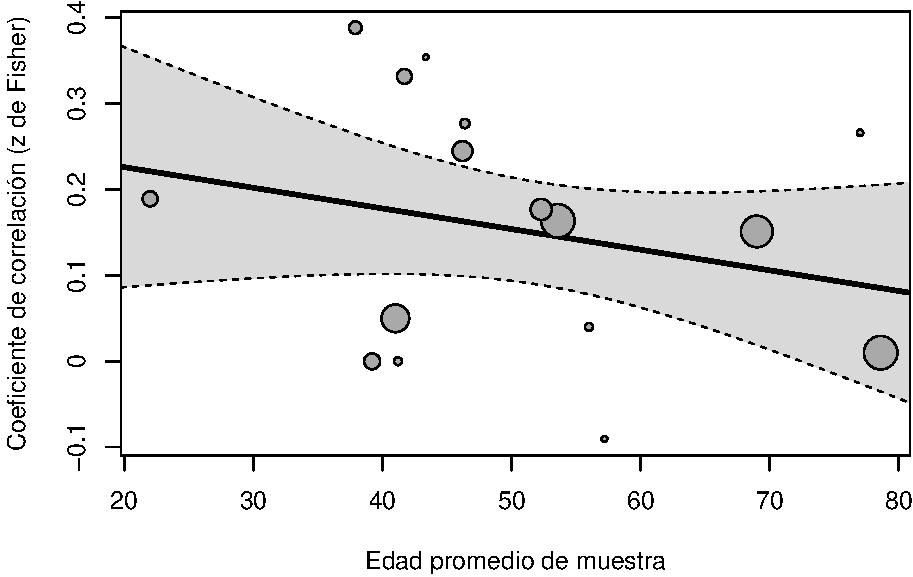
\includegraphics{Meta-analysis_files/figure-latex/reg-plot1-1.pdf}
\caption{\label{fig:reg-plot1}Gráfico de dispersión meta-analítico (\emph{Meta-Analytic Scatter Plot}). El tamaño de los puntos es proporcional al peso que recibieron los estudios en el meta-análisis (puntos más grandes para los estudios con más peso, pues tienen un tamaño de muestra mayor y con un menor error estimado). La línea negra representa el efecto previsto en función del predictor (en este caso \texttt{meanage}, edad promedio), que por supuesto coincide con las predicciones del objeto \texttt{pred.res.modage} (Output 11, en la sección \ref{pred-mods}); la banda gris demilimata por líneas punteadas representa el intervalo de confianza del 95\%.}
\end{figure}

\hypertarget{plot-mod}{%
\subsubsection{\texorpdfstring{\emph{Forest plot} y \emph{funnel plot}}{Forest plot y funnel plot}}\label{plot-mod}}

Por supuesto, de estos resultados también puedo crear \emph{forest plots} y \emph{funnel plots}, siguiendo los ejemplos y código de la sección \ref{meta-cor}. Para el \emph{forest plot}, hago a continuación un ejemplo anotado y mejorado\footnote{La función \href{https://cran.r-project.org/web/packages/metaviz/vignettes/metaviz.html\#creating-forest-plots-with-function-viz_forest}{\texttt{viz\_forest}} del paquete \href{https://cran.r-project.org/web/packages/metaviz/vignettes/metaviz.html}{\texttt{metaviz}} no puede crear un \emph{forest plot} de un meta-análisis ajustado con \texttt{metafor} cuando este modelo contiene variables moderadoras continuas, o cuando tiene como variable moderadora más de una variable categórica. En otras palabras, solo podrá hacer el \emph{forest plot} si nuestro meta-análisis no tiene moderadores, o tiene un único moderador categórico. Como en este ejemplo nuestro moderador es una variable continua, no es posible usar esta función.} (Fig. \ref{fig:for-plot-mod1}, con un código similar al usado como ejemplo en la Fig. \ref{fig:for-plot2}). Sin embargo, es importante tener en cuenta que esta opción no creará un resumen del meta-análisis, ya que no tenemos un solo efecto \emph{real} como producto del meta-análisis.

\begin{Shaded}
\begin{Highlighting}[]
\CommentTok{\# forest plot con anotaciones adicionales}
\FunctionTok{forest}\NormalTok{(res.modage,  }\AttributeTok{cex =} \FloatTok{0.75}\NormalTok{, }\AttributeTok{xlim =} \FunctionTok{c}\NormalTok{(}\SpecialCharTok{{-}}\FloatTok{1.6}\NormalTok{, }\FloatTok{1.6}\NormalTok{),}
       \AttributeTok{slab =} \FunctionTok{paste}\NormalTok{(dat}\SpecialCharTok{$}\NormalTok{authors, dat}\SpecialCharTok{$}\NormalTok{year, }\AttributeTok{sep =} \StringTok{", "}\NormalTok{),}
       \AttributeTok{showweights =} \ConstantTok{TRUE}\NormalTok{,}
       \AttributeTok{xlab =} \StringTok{"Coeficiente de correlación transformado en z de Fisher"}\NormalTok{,}
       \AttributeTok{digits =} \FunctionTok{c}\NormalTok{(}\DecValTok{2}\NormalTok{,3L))}
\CommentTok{\# agregar encabezados a las columnas (valores de X y Y deben ser ajustados)}
\FunctionTok{par}\NormalTok{(}\AttributeTok{cex =} \FloatTok{0.8}\NormalTok{, }\AttributeTok{font =} \DecValTok{2}\NormalTok{)}
\FunctionTok{text}\NormalTok{(}\AttributeTok{x =} \SpecialCharTok{{-}}\FloatTok{1.6}\NormalTok{, }\AttributeTok{y =} \DecValTok{18}\NormalTok{, }\AttributeTok{labels =} \StringTok{"Autor(es), Año"}\NormalTok{, }\AttributeTok{pos =} \DecValTok{4}\NormalTok{)}
\FunctionTok{text}\NormalTok{(}\AttributeTok{x =} \DecValTok{0}\NormalTok{, }\AttributeTok{y =} \DecValTok{18}\NormalTok{, }\AttributeTok{labels =} \StringTok{"Efecto e IC"}\NormalTok{, }\AttributeTok{pos =} \DecValTok{4}\NormalTok{)}
\FunctionTok{text}\NormalTok{(}\AttributeTok{x =} \DecValTok{1}\NormalTok{, }\AttributeTok{y =} \DecValTok{18}\NormalTok{, }\AttributeTok{labels =} \StringTok{"Peso"}\NormalTok{, }\AttributeTok{pos =} \DecValTok{2}\NormalTok{)}
\FunctionTok{text}\NormalTok{(}\AttributeTok{x =} \FloatTok{1.6}\NormalTok{, }\AttributeTok{y =} \DecValTok{18}\NormalTok{, }\AttributeTok{labels =} \StringTok{"Corr. [95\% IC]"}\NormalTok{, }\AttributeTok{pos =} \DecValTok{2}\NormalTok{)}
\end{Highlighting}
\end{Shaded}

\begin{figure}
\centering
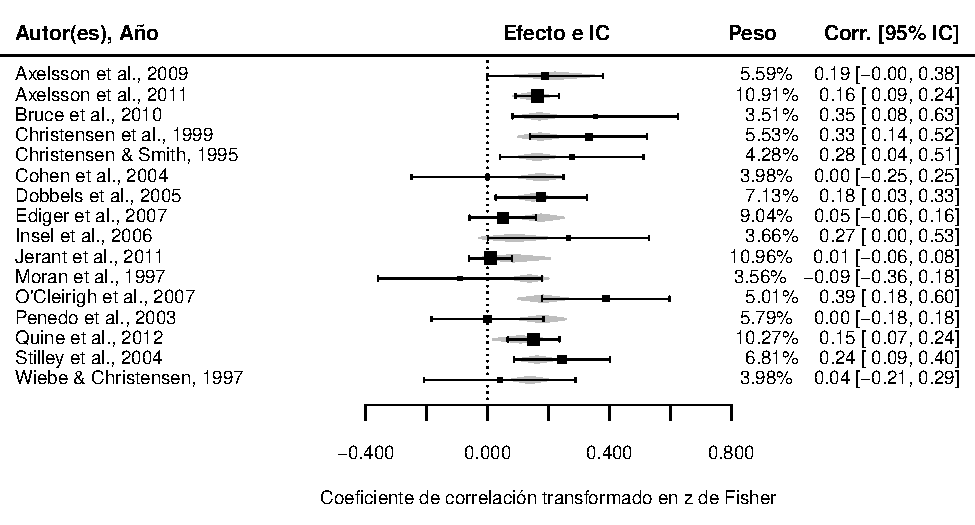
\includegraphics{Meta-analysis_files/figure-latex/for-plot-mod1-1.pdf}
\caption{\label{fig:for-plot-mod1}\emph{Forest plot} básico de \href{https://www.metafor-project.org/doku.php}{metafor}, para un meta-análisis incluyendo la edad promedio de los participantes como moderador. En la ilustración gráfica, además de los efectos originales, se puede ver el efecto de cada estudio estimado cuando se incluye el moderador como polígonos (diamantes) de color gris. Sin embargo, ya no obtenemos una fila al final representando el efecto promediado del meta-análisis, ya que no tenemos un solo efecto.}
\end{figure}

De manera similar, podemos obtener un \emph{funnel plot} de nuestro meta-análisis con moderador. Es importante tener en cuenta que tanto el paquete \texttt{weightr} como el paquete \texttt{metafor} tienen funciones llamadas \texttt{funnel}. Dado que cargamos el paquete \texttt{weightr} después, R por defecto intentará intentará crear el \emph{funnel plot} con la función \texttt{funnel} del paquete \texttt{weightr}, en vez de la función \texttt{funnel} del paquete \texttt{metafor}. Para evitar este error, tenemos dos opciones: podemos pedirle a R explícitamente que use la función \texttt{funnel} del paquete \texttt{metafor} con el comando \texttt{metafor::funnel}, o podemos pedirle a R que elimine el paquete de la memoria con la función \texttt{detach("package:metameta",\ unload\ =\ TRUE)}. En este caso, usaré la primera opción.

Este \emph{funnel plot}, a diferencia los los anteriores, nos mostrará los valores residuales de cada estudio (es decir, qué tanto se alejan del resultado de nuestro meta-análisis, que tiene un valor residual de 0; Fig. \ref{fig:funnel-plot1}), en vez de los coeficientes de correlación (transformados a \(z\) de Fisher).

\begin{Shaded}
\begin{Highlighting}[]
\NormalTok{metafor}\SpecialCharTok{::}\FunctionTok{funnel}\NormalTok{(res.modage,}
                \AttributeTok{xlab =} \StringTok{"Valor residual"}\NormalTok{,}
                \AttributeTok{ylab =} \StringTok{"Error estándar"}\NormalTok{)}
\end{Highlighting}
\end{Shaded}

\begin{figure}
\centering
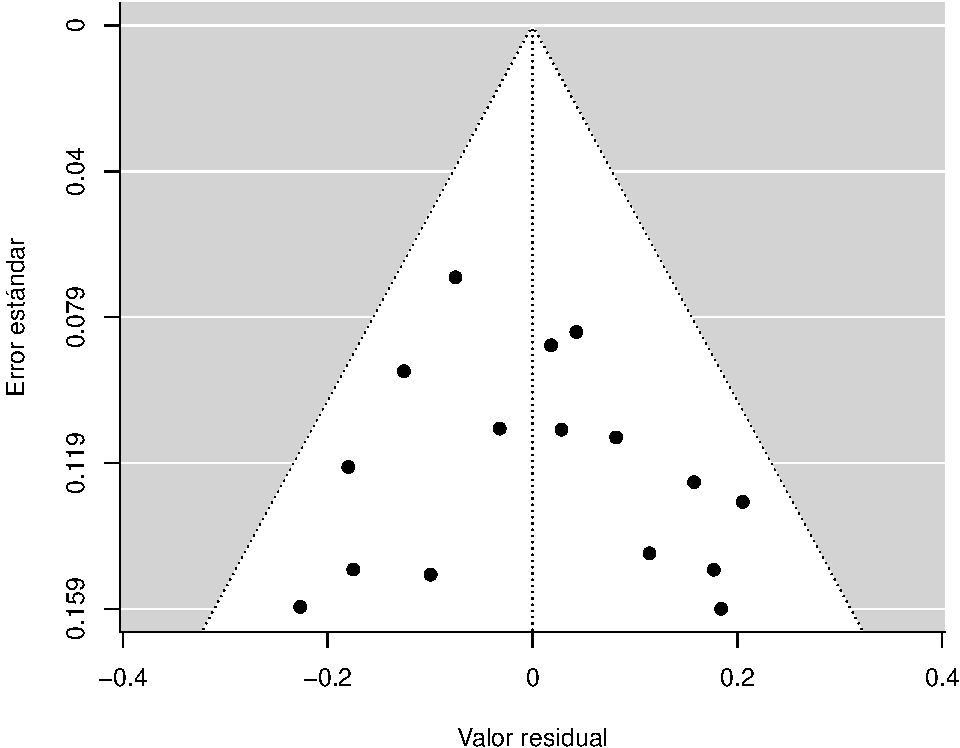
\includegraphics{Meta-analysis_files/figure-latex/funnel-plot-mod1-1.pdf}
\caption{\label{fig:funnel-plot-mod1}\emph{Funnel plot} básico de \href{https://www.metafor-project.org/doku.php}{metafor}, para un meta-análisis incluyendo la edad promedio de los participantes como moderador, y con títulos de los ejes en español. La línea punteada vertical representa el efecto meta-analizado que hemos encontrado, así que podemos ver los estudios que encontraron un efecto mayor (derecha de la línea punteada) o menor (izquierda) de éste. \textbf{Nota}: Para evitar confunción entre las funciones \texttt{funnel} de los paquetes \texttt{weightr} y \texttt{metafor}, en este caso he usado el comando \texttt{metafor::funnel} para pedirle a R explícitamente que use la función \texttt{funnel} del paquete \texttt{metafor}.}
\end{figure}

\hypertarget{ejemplo-2-moderaciuxf3n-de-una-variable-categuxf3rica-controles-usados-en-cada-estudio-meta-analizado}{%
\subsection{Ejemplo 2: Moderación de una variable categórica (controles usados en cada estudio meta-analizado)}\label{ejemplo-2-moderaciuxf3n-de-una-variable-categuxf3rica-controles-usados-en-cada-estudio-meta-analizado}}

Como segundo ejemplo, voy a mirar si el hecho de que los estudios tengan variables que fueron controladas, modera la asociación entre concienciación (\emph{conscientiousness}) y adherencia a la medicación prescrita. Siguiendo los mismos pasos, voy hacer éste análisis, pero voy a asignar este meta-análisis a un objeto llamado \texttt{res.contr}.

\begin{Shaded}
\begin{Highlighting}[]
\NormalTok{res.contr }\OtherTok{\textless{}{-}} \FunctionTok{rma}\NormalTok{(}\AttributeTok{yi =}\NormalTok{ yi, }\AttributeTok{vi =}\NormalTok{ vi, }\AttributeTok{mods =} \SpecialCharTok{\textasciitilde{}}\NormalTok{controls, }\AttributeTok{data =}\NormalTok{ dat)}
\NormalTok{res.contr}
\end{Highlighting}
\end{Shaded}

\begin{ROut}{Consola de R: Output~\thetcbcounter}
                \begin{footnotesize}
                \begin{verbatim} 
Mixed-Effects Model (k = 16; tau^2 estimator: REML)

tau^2 (estimated amount of residual heterogeneity):     0.0000 (SE = 0.0015)
tau (square root of estimated tau^2 value):             0.0002
I^2 (residual heterogeneity / unaccounted variability): 0.00%
H^2 (unaccounted variability / sampling variability):   1.00
R^2 (amount of heterogeneity accounted for):            100.00%

Test for Residual Heterogeneity:
QE(df = 14) = 18.0370, p-val = 0.2051

Test of Moderators (coefficient 2):
QM(df = 1) = 20.1221, p-val < .0001

Model Results:

                  estimate      se     zval    pval    ci.lb    ci.ub      
intrcpt             0.1788  0.0208   8.6044  <.0001   0.1380   0.2195  *** 
controlsmultiple   -0.1621  0.0361  -4.4858  <.0001  -0.2329  -0.0913  *** 

---
Signif. codes:  0 '***' 0.001 '**' 0.01 '*' 0.05 '.' 0.1 ' ' 1
 \end{verbatim}
                \end{footnotesize}
                \end{ROut}

En éste caso, a diferencia del ejemplo de moderación anteriores, la variable moderadora (\texttt{controls}) sí tiene un efecto significativo, como se puede ver en la columna \texttt{pval} para el efecto de \texttt{controlsnone} (\textless0.001), y en los asteriscos que aparecen al final de esa fila (\texttt{***}).

\hypertarget{pred-mods2}{%
\subsubsection{Más información e interpretación de la moderación}\label{pred-mods2}}

\begin{Shaded}
\begin{Highlighting}[]
\NormalTok{pred.res.contr }\OtherTok{\textless{}{-}} \FunctionTok{predict}\NormalTok{(res.contr, }\AttributeTok{newmods =} \FunctionTok{c}\NormalTok{(}\DecValTok{0}\NormalTok{, }\DecValTok{1}\NormalTok{)) }\SpecialCharTok{\%\textgreater{}\%} 
  \FunctionTok{as.data.frame}\NormalTok{() }\SpecialCharTok{\%\textgreater{}\%} 
  \FunctionTok{mutate\_all}\NormalTok{(}\SpecialCharTok{\textasciitilde{}}\FunctionTok{round}\NormalTok{(., }\DecValTok{3}\NormalTok{)) }\SpecialCharTok{\%\textgreater{}\%}
  \FunctionTok{mutate}\NormalTok{(}\AttributeTok{controls =} \FunctionTok{levels}\NormalTok{(dat}\SpecialCharTok{$}\NormalTok{controls)) }\SpecialCharTok{\%\textgreater{}\%} 
  \FunctionTok{rename}\NormalTok{(}\AttributeTok{yi =}\NormalTok{ pred) }\SpecialCharTok{\%\textgreater{}\%} 
  \FunctionTok{select}\NormalTok{(}\DecValTok{7}\NormalTok{, }\DecValTok{1}\SpecialCharTok{:}\DecValTok{6}\NormalTok{)}
\NormalTok{pred.res.contr}
\end{Highlighting}
\end{Shaded}

\begin{ROut}{Consola de R: Output~\thetcbcounter}
                \begin{footnotesize}
                \begin{verbatim}   controls    yi    se  ci.lb ci.ub  pi.lb pi.ub
1     none 0.179 0.021  0.138 0.219  0.138 0.219
2 multiple 0.017 0.030 -0.041 0.075 -0.041 0.075
 \end{verbatim}
                \end{footnotesize}
                \end{ROut}

\hypertarget{meta-analytic-scatter-plot-gruxe1fico-de-dispersiuxf3n-meta-analuxedtico-1}{%
\paragraph{\texorpdfstring{\emph{Meta-Analytic Scatter Plot} (Gráfico de dispersión meta-analítico)}{Meta-Analytic Scatter Plot (Gráfico de dispersión meta-analítico)}}\label{meta-analytic-scatter-plot-gruxe1fico-de-dispersiuxf3n-meta-analuxedtico-1}}

Al igual que en el ejemplo de meta-análisis con moderación de una variable continua (sección @ref(ex.mod1)), es posible hacer un gráfico de dispersión meta-analítico (\emph{meta-analytic scatter plot}) usando la función \texttt{regplot} del paquete \texttt{metafor}. Sin embargo, dado que la variable moderadora es categórica, el modelo genera variables \emph{dummy} asignando valores de 0 y 1 a los niveles de esta variable (en este caso, 0 = ningún control; 1 = múltiples controles). Por esto, en el ejemplo a continuación agregué a la descripción del eje \(X\) esta información.

\begin{Shaded}
\begin{Highlighting}[]
\FunctionTok{regplot}\NormalTok{(res.contr,}
        \AttributeTok{ylab =} \StringTok{"Coeficiente de correlación transformado en z de Fisher"}\NormalTok{,}
        \AttributeTok{xlab =} \StringTok{"Controles (0 = ninguno; 1 = múltiples)"}\NormalTok{)}
\end{Highlighting}
\end{Shaded}

\begin{figure}
\centering
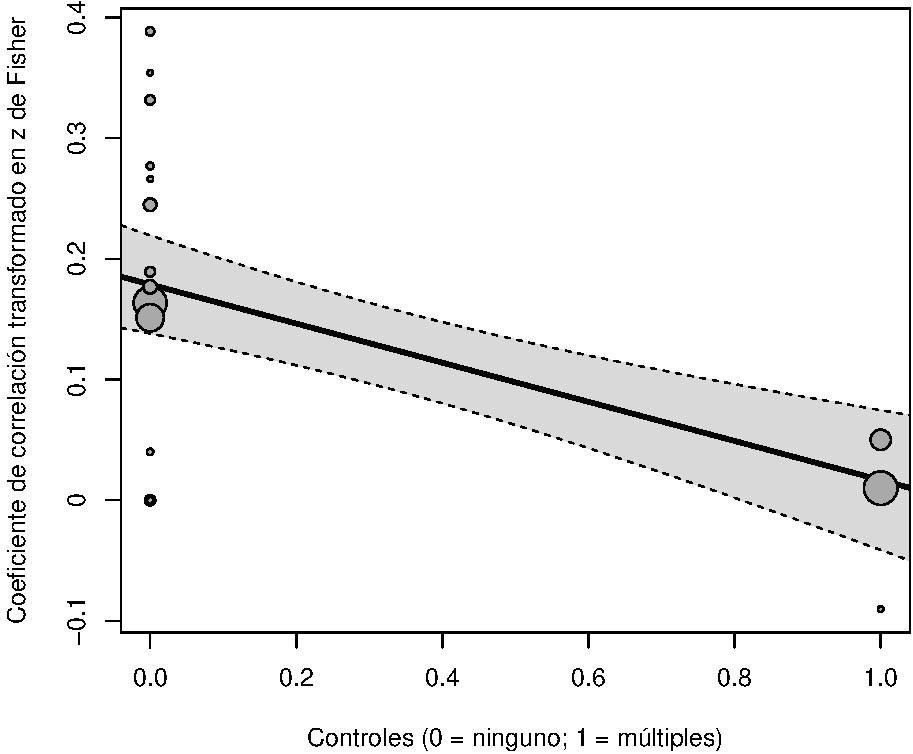
\includegraphics{Meta-analysis_files/figure-latex/reg-plot2-1.pdf}
\caption{\label{fig:reg-plot2}Gráfico de dispersión meta-analítico (\emph{Meta-Analytic Scatter Plot}) básico de \href{https://www.metafor-project.org/doku.php}{metafor} creado con la función \texttt{regplot}. El tamaño de los puntos es proporcional al peso que recibieron los estudios en el meta-análisis (puntos más grandes para los estudios con más peso, pues tienen un tamaño de muestra mayor y con un menor error estimado). La línea negra representa el efecto previsto en función del predictor (en este caso \texttt{controls}, controles). La banda gris demilimata por líneas punteadas representa el intervalo de confianza del 95\%. Dado que la variable moderadora es categórica, el modelo genera variables \emph{dummy} asignando valores de 0 y 1 a los niveles de esta variable (en este caso, 0 = ningúun control; 1 = múltiples controles), tal y como se describe en el eje \emph{X}. Para una versión más apropiada, ver Fig. \ref{fig:reg-plot3}.}
\end{figure}

Aunque la figura \ref{fig:reg-plot2} presenta información correcta, tal vez no es la más adecuada ni la más clara cuando se trata de representar meta-análisis con moderadores categóricos. Por ejemplo, a pesar de que nuestro moderador es un factor (controles) con dos niveles (ninguno, múltiples), en el eje \(X\) se representa como una variable continua con valores entre 0 y 1, que además tiene valores intermedios (0.2, 2.4, 0.6, 0.8) que en nuestro caso no tienen sentido.

Sin embargo, de manera un poco más \emph{artesanal}, es posible crear una versión más adecuada usando, por ejemplo, \texttt{ggplot2}. El código siguiente permite crear una figura bastante sofisticada usando éste paquete.

\begin{Shaded}
\begin{Highlighting}[]
\CommentTok{\# Definir base de datos, así como ejes X (controls) y Y (yi)}
\FunctionTok{ggplot}\NormalTok{(dat, }\FunctionTok{aes}\NormalTok{(}\AttributeTok{x =}\NormalTok{ controls, }\AttributeTok{y =}\NormalTok{ yi)) }\SpecialCharTok{+}
  \CommentTok{\# Agregar puntos para cada estudio, con tamaño y color según tamaño de muestra (ni)}
  \FunctionTok{geom\_point}\NormalTok{(}\FunctionTok{aes}\NormalTok{(}\AttributeTok{size =}\NormalTok{ ni, }\AttributeTok{color =}\NormalTok{ ni),}
             \AttributeTok{alpha =} \FloatTok{0.5}\NormalTok{) }\SpecialCharTok{+}
  \CommentTok{\# Definir escala de colores}
  \FunctionTok{scale\_colour\_gradient}\NormalTok{(}\AttributeTok{low =} \StringTok{"red"}\NormalTok{,}
                        \AttributeTok{high =} \StringTok{"blue"}\NormalTok{) }\SpecialCharTok{+}
  \CommentTok{\# Definir rango de tamaño de los puntos}
  \FunctionTok{scale\_size\_continuous}\NormalTok{(}\AttributeTok{range =} \FunctionTok{c}\NormalTok{(}\DecValTok{1}\NormalTok{, }\DecValTok{10}\NormalTok{)) }\SpecialCharTok{+}
  \CommentTok{\# Combinar leyendas de colores y tamaños de puntos en una sola leyenda}
  \FunctionTok{guides}\NormalTok{(}\AttributeTok{color =} \FunctionTok{guide\_legend}\NormalTok{(), }
         \AttributeTok{size =} \FunctionTok{guide\_legend}\NormalTok{()) }\SpecialCharTok{+}
  \CommentTok{\# Traducir etiquetas del eje X en español}
  \FunctionTok{scale\_x\_discrete}\NormalTok{(}\AttributeTok{labels=}\FunctionTok{c}\NormalTok{(}\StringTok{"none"} \OtherTok{=} \StringTok{"Ninguno"}\NormalTok{, }
                            \StringTok{"multiple"} \OtherTok{=} \StringTok{"Múltiples"}\NormalTok{)) }\SpecialCharTok{+}
  \CommentTok{\# Cambiar títulos de ejes a español}
  \FunctionTok{labs}\NormalTok{(}\AttributeTok{x =} \StringTok{"Controles"}\NormalTok{, }
       \AttributeTok{y =} \StringTok{"Coeficiente de correlación }\SpecialCharTok{\textbackslash{}n}\StringTok{transformado en z de Fisher "}\NormalTok{) }\SpecialCharTok{+}
  \CommentTok{\# Agregar barras de error para cada categoría, con base en predicción hecha en sección 4.2.1}
  \FunctionTok{geom\_errorbar}\NormalTok{(}\AttributeTok{data =}\NormalTok{ pred.res.contr,}
                \AttributeTok{mapping =} \FunctionTok{aes}\NormalTok{(}\AttributeTok{ymin =}\NormalTok{ ci.lb, }\AttributeTok{ymax =}\NormalTok{ ci.ub),}
                \AttributeTok{width =} \FloatTok{0.1}\NormalTok{,}
                \AttributeTok{color =} \StringTok{"black"}\NormalTok{) }\SpecialCharTok{+}
  \CommentTok{\# Agregar puntos blancos representando predicción para cada categoría hecha en sección 4.2.1}
  \FunctionTok{geom\_point}\NormalTok{(}\AttributeTok{data =}\NormalTok{ pred.res.contr,}
             \AttributeTok{shape =} \DecValTok{21}\NormalTok{, }\AttributeTok{size =} \DecValTok{3}\NormalTok{,}
             \AttributeTok{color =} \StringTok{"black"}\NormalTok{, }\AttributeTok{fill =} \StringTok{"white"}\NormalTok{) }\SpecialCharTok{+}
  \CommentTok{\# Cambiar tptitulo de leyenda}
  \FunctionTok{labs}\NormalTok{(}\AttributeTok{color =} \StringTok{"Tamaño de }\SpecialCharTok{\textbackslash{}n}\StringTok{muestra"}\NormalTok{,}
       \AttributeTok{size =} \StringTok{"Tamaño de }\SpecialCharTok{\textbackslash{}n}\StringTok{muestra"}\NormalTok{)}
\end{Highlighting}
\end{Shaded}

El código anterior puede verse algo confuso para quien no haya usado \texttt{ggplot2} antes. Por esto, he agregado anotaciones, función por función, para ayudar a su interpretación\footnote{Debido a sus enormes y numerosas posibilidades, \texttt{ggplot2} es quizás la opción más poderosa para hacer gráficos estadísticos en R; por esto explicar sus bases supera por mucho el alcance de esta guía, y posiblemente requeriría múltiples tutoriales independientes. Sin embargo, hay gran cantidad de opciones disponibles en internet. Por ejemplo, puedes leer este \href{https://rpubs.com/anlope10/562981}{tutorial} (\protect\hyperlink{ref-lopezpenarandaTutorialGgplot22019}{López Peñaranda, 2019}) o ver este \href{https://youtu.be/BUzTAr_QqKs}{video} (\protect\hyperlink{ref-datademiaAprendeGgplot22018}{Datademia, 2018}).}. Este código produce la figura \ref{fig:reg-plot3}.

\begin{figure}
\centering
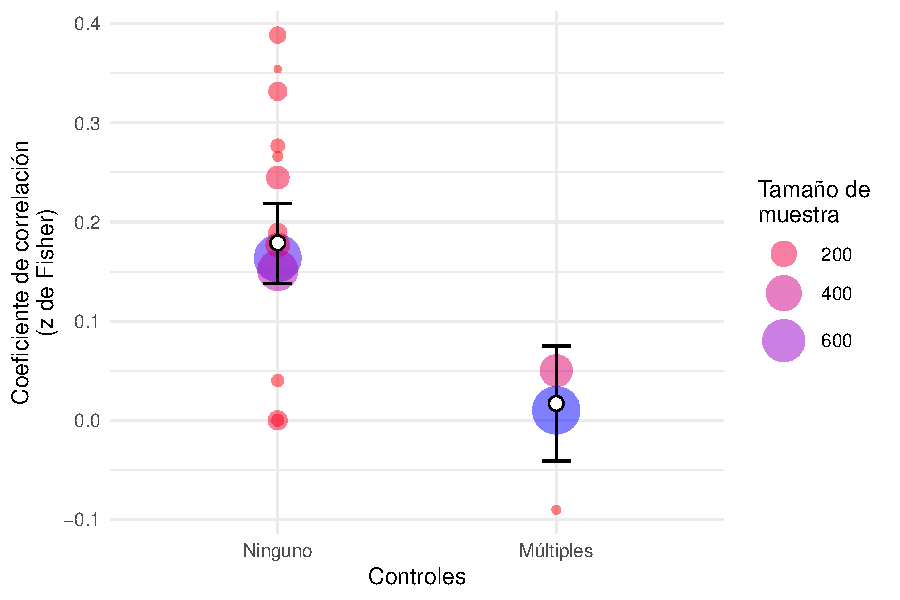
\includegraphics{Meta-analysis_files/figure-latex/reg-plot3-1.pdf}
\caption{\label{fig:reg-plot3}Gráfico de dispersión meta-analítico (\emph{Meta-Analytic Scatter Plot}) creado manualmente con \href{https://ggplot2.tidyverse.org/}{ggplot2} para hacer una mejor representación de un moderador categírico. Los puntos de colores representan el coeficiente de correlación en función de la presencia o ausencia de controles. El tamaño de los puntos es proporcional al tamaño de muestra de los estudios inluidos en el meta-análisis (puntos más grandes y azules para los estudios con mayor tamaño de muestra). Los puntos blancos superpuetos representan el efecto estimado para cada categoría, y las barras de error representan los intervalos de confianza del 95\%.}
\end{figure}

\hypertarget{plot-mod2}{%
\subsubsection{\texorpdfstring{\emph{Forest plot} y \emph{funnel plot}}{Forest plot y funnel plot}}\label{plot-mod2}}

Por supuesto, \emph{forest plots} y \emph{funnel plots} pueden ser creados, tal y como describí en la sección \ref{plot-mod}.

\hypertarget{conclusiones-y-recomendaciones-generales}{%
\section{Conclusiones y recomendaciones generales}\label{conclusiones-y-recomendaciones-generales}}

Hacer un meta-análisis de correlación en R no es complejo. Sin embargo, la confiabilidad del resultado que te proporcione, dependerá de varios aspectos.

Primero, debes tener hacer una selección de artículos buena y no sesgada. Esto típicamente incluye:

\begin{enumerate}
\def\labelenumi{\arabic{enumi})}
\item
  Formular la pregunta de investigación clara, con base en teoría
\item
  Identificar la bibliografía pertinente
\item
  Extraer y consolidar los datos de los estudios (en el caso de correlaciones, cuando menos \emph{r} y \emph{n})
\end{enumerate}

Con esto deberías ya poder hacer una base de datos para un meta-análisis de correlación simple. Mientras tengas en tu base de datos algún identificador de cada estudio, el tamaño de efecto (\emph{r}) y el tamaño de muestra (\emph{n}), tendrías todo lo necesario para hacerlo. Por ejemplo:

\begin{longtable}[]{@{}lll@{}}
\toprule()
estudio & ri & ni \\
\midrule()
\endhead
Autores (año) & 0.25 & 425 \\
Autores (año) & 0.65 & 45 \\
Autores (año) & 0.12 & 235 \\
\bottomrule()
\end{longtable}

Adicionalmente, podrías tomar o extraer información de posibles variables moderadoras; por ejemplo, si los estudios se pudieran agrupar según metodología usada o población estudiada, y sospechas que estas variables afectan la correlación encontrada en cada estudio, podrías agregar esta información en una o más variables.

Una vez tengas tu base de datos lista, deberías, cuando menos:

\begin{enumerate}
\def\labelenumi{\arabic{enumi}.}
\tightlist
\item
  Hacer el meta-análisis
\end{enumerate}

\begin{itemize}
\item
  Reportar información sobre heterogeneidad
\item
  Incluir un diagnóstico de influencia
\item
  Reportar los resultados usando un \emph{forest plot} (diagrama de bosque)
\item
  Mostrar la distribución de los resultados en un \emph{funnel plot} (diagrama de embudo) y estimar el sesgo de estudios pequeños
\end{itemize}

\begin{enumerate}
\def\labelenumi{\arabic{enumi}.}
\setcounter{enumi}{1}
\tightlist
\item
  Estimar si hay evidencia de sesgo de publicación
\end{enumerate}

\begin{itemize}
\tightlist
\item
  Puedes usar el método \emph{trim and fill} (recorte y relleno) o, lo que es mejor, hacer una estimación del modelo de función de peso
\end{itemize}

Adicionalmente, podrías:

\begin{enumerate}
\def\labelenumi{\arabic{enumi}.}
\setcounter{enumi}{2}
\item
  Estimar el poder estadístico del meta-análisis y los estudios meta-analizados
\item
  Hacer un meta-análisis combinatorio)
\end{enumerate}

\newpage

\hypertarget{referencias}{%
\section{Referencias}\label{referencias}}

\hypertarget{refs}{}
\begin{CSLReferences}{1}{0}
\leavevmode\vadjust pre{\hypertarget{ref-SesgoPublicacion2008}{}}%
{Acerca del sesgo de publicación en literatura sobre antidepresivos}. (2008). \emph{Revista Colombiana de Psiquiatría}, \emph{37}(1), 8--10. \url{http://ref.scielo.org/sp52pr}

\leavevmode\vadjust pre{\hypertarget{ref-magrittrcite}{}}%
Bache, S. M., \& Wickham, H. (2022). \emph{{magrittr}: A forward-pipe operator for {R}}. \url{https://CRAN.R-project.org/package=magrittr}

\leavevmode\vadjust pre{\hypertarget{ref-BalduzziMeta2019}{}}%
Balduzzi, S., Rücker, G., \& Schwarzer, G. (2019). How to perform a meta-analysis with {R}: A practical tutorial. \emph{Evidence-Based Mental Health}, \emph{22}, 153--160. \url{https://doi.org/10.1136/ebmental-2019-300117}

\leavevmode\vadjust pre{\hypertarget{ref-belsleyRegressionDiagnosticsIdentifying1980}{}}%
Belsley, D. A., Kuh, E., \& Welsch, R. E. (1980). \emph{Regression {Diagnostics}: {Identifying Influential Data} and {Sources} of {Collinearity}}. {John Wiley \& Sons, Inc.} \url{https://doi.org/10.1002/0471725153}

\leavevmode\vadjust pre{\hypertarget{ref-borensteinIdentifyingQuantifyingHeterogeneity2009}{}}%
Borenstein, M., Hedges, L. V., Higgns, J. P. T., \& Rothstein, H. R. (2009). Identifying and {Quantifying Heterogeneity}. In \emph{Introduction to {Meta}-{Analysis}} (pp. 107--125). Wiley. \url{https://doi.org/10.1002/9780470743386.ch16}

\leavevmode\vadjust pre{\hypertarget{ref-coburnPublicationBiasFunction2015}{}}%
Coburn, K. M., \& Vevea, J. L. (2015). Publication bias as a function of study characteristics. \emph{Psychological Methods}, \emph{20}(3), 310--330. \url{https://doi.org/10.1037/met0000046}

\leavevmode\vadjust pre{\hypertarget{ref-coburnWeightr2019}{}}%
Coburn, K. M., \& Vevea, J. L. (2019). \emph{Weightr: Estimating weight-function models for publication bias}. \url{https://CRAN.R-project.org/package=weightr}

\leavevmode\vadjust pre{\hypertarget{ref-cookDetectionInfluentialObservation1977}{}}%
Cook, R. D. (1977). Detection of {Influential Observation} in {Linear Regression}. \emph{Technometrics}, \emph{19}(1), 15--18. \url{https://doi.org/10.2307/1268249}

\leavevmode\vadjust pre{\hypertarget{ref-cookResidualsInfluenceRegression1982}{}}%
Cook, R. D., \& Weisberg, S. (1982). \emph{Residuals and {Influence} in {Regression}}. {New York: Chapman and Hall}. \url{https://hdl.handle.net/11299/37076}

\leavevmode\vadjust pre{\hypertarget{ref-datademiaAprendeGgplot22018}{}}%
Datademia. (2018). \emph{Aprende {Ggplot2} en {R} \emph{{[}video{]}}}. YouTube. \url{https://youtu.be/BUzTAr_QqKs}.

\leavevmode\vadjust pre{\hypertarget{ref-duvalTrimFillMethod2005}{}}%
Duval, S. (2005). The {Trim} and {Fill Method}. In H. R. Rothstein, A. J. Sutton, \& M. Borenstein (Eds.), \emph{Publication {Bias} in {Meta-Analysis}} (pp. 127--144). {John Wiley \& Sons}. \url{https://doi.org/10.1002/0470870168.ch8}

\leavevmode\vadjust pre{\hypertarget{ref-duvalNonparametricTrimFill2000}{}}%
Duval, S., \& Tweedie, R. (2000a). A {Nonparametric} {``{Trim} and {Fill}''} {Method} of {Accounting} for {Publication Bias} in {Meta-Analysis}. \emph{Journal of the American Statistical Association}, \emph{95}(449), 89--98. \url{https://doi.org/10.1080/01621459.2000.10473905}

\leavevmode\vadjust pre{\hypertarget{ref-duvalTrimFillSimple2000}{}}%
Duval, S., \& Tweedie, R. (2000b). Trim and {Fill}: {A Simple Funnel-Plot-Based Method} of {Testing} and {Adjusting} for {Publication Bias} in {Meta-Analysis}. \emph{Biometrics}, \emph{56}(2), 455--463. \url{https://doi.org/10.1111/j.0006-341X.2000.00455.x}

\leavevmode\vadjust pre{\hypertarget{ref-eggerBiasMetaanalysisDetected1997}{}}%
Egger, M., Smith, G. D., Schneider, M., \& Minder, C. (1997). {Bias in Meta-Analysis Detected by a Simple, Graphical Test}. \emph{BMJ}, \emph{315}(7109), 629--634. \url{https://doi.org/10.1136/bmj.315.7109.629}

\leavevmode\vadjust pre{\hypertarget{ref-fisherFrequencyDistributionValues1915}{}}%
Fisher, R. A. (1915). Frequency {Distribution} of the {Values} of the {Correlation Coefficient} in {Samples} from an {Indefinitely Large Population}. \emph{Biometrika}, \emph{10}(4), 507--521. \url{https://doi.org/10.2307/2331838}

\leavevmode\vadjust pre{\hypertarget{ref-harrer2021doing}{}}%
Harrer, M., Cuijpers, P., A, F. T., \& Ebert, D. D. (2021). \emph{{Doing Meta-Analysis With {R}: A Hands-On Guide}} (1st ed.). Chapman \& Hall/CRC Press. \url{https://bookdown.org/MathiasHarrer/Doing_Meta_Analysis_in_R/}

\leavevmode\vadjust pre{\hypertarget{ref-Harrer2019dmetar}{}}%
Harrer, M., Cuijpers, P., Furukawa, T., \& Ebert, D. D. (2019). \emph{{dmetar: Companion R Package For The Guide 'Doing Meta-Analysis in R'}}. \url{http://dmetar.protectlab.org/}

\leavevmode\vadjust pre{\hypertarget{ref-Henry2003}{}}%
Henry, N. W., Cohen, J., \& Cohen, P. (2003). \emph{Applied {Multiple Regression}/{Correlation Analysis} for the {Behavioral Sciences}.} (3rd ed.). {Lawrence Erlbaum Associates}. \url{https://doi.org/10.4324/9780203774441}

\leavevmode\vadjust pre{\hypertarget{ref-johnBigFiveTrait1999}{}}%
John, O. P., \& Srivastava, S. (1999). The {Big Five Trait} taxonomy: {History}, measurement, and theoretical perspectives. In L. A. Pervin \& O. P. John (Eds.), \emph{Handbook of personality: {Theory} and research, 2nd ed} (pp. 102--138). {Guilford Press}. \url{http://jenni.uchicago.edu/econ-psych-traits/John_Srivastava_1995_big5.pdf}

\leavevmode\vadjust pre{\hypertarget{ref-KossmeierMetaviz}{}}%
Kossmeier, M., Tran, U. S., \& Voracek, M. (2020). \emph{{metaviz: Forest Plots, Funnel Plots, and Visual Funnel Plot Inference for Meta-Analysis}}. \url{https://CRAN.R-project.org/package=metaviz}

\leavevmode\vadjust pre{\hypertarget{ref-leongomezMetaanalysis2021}{}}%
Leongómez, J. D. (2021). \emph{Hacer meta-análisis en jamovi es muy fácil \emph{{[}video{]}}}. YouTube. \url{https://youtu.be/ntBbkOn9D_o}.

\leavevmode\vadjust pre{\hypertarget{ref-leongomezAnalisisPoderEstadistico2020}{}}%
Leongómez, J. D. (2020a). \emph{Análisis de poder estadístico y cálculo de tamaño de muestra en {R}: {Guía} práctica}. {Zenodo}. \url{https://doi.org/10.5281/zenodo.3988776}

\leavevmode\vadjust pre{\hypertarget{ref-leongomezPoderRvid2020}{}}%
Leongómez, J. D. (2020b). \emph{Poder estadístico y tamaño de muestra en {R} \emph{{[}serie de videos{]}}}. YouTube. \url{https://youtube.com/playlist?list=PLHk7UNt35ccVdyHqnQ6oXVYA6JBNFrE1x}.

\leavevmode\vadjust pre{\hypertarget{ref-lopezpenarandaTutorialGgplot22019}{}}%
López Peñaranda, A. (2019). \emph{Tutorial de ggplot2}. RPubs. \url{https://rpubs.com/anlope10/562981}.

\leavevmode\vadjust pre{\hypertarget{ref-Manterola2019}{}}%
Manterola, C., Quiroz, G., Salazar, P., \& García, N. (2019). Metodología de los tipos y diseños de estudio más frecuentemente utilizados en investigación clínica. \emph{Revista Médica Clínica Las Condes}, \emph{30}(1), 36--49. https://doi.org/\url{https://doi.org/10.1016/j.rmclc.2018.11.005}

\leavevmode\vadjust pre{\hypertarget{ref-molloy2013}{}}%
Molloy, G. J., O'Carroll, R. E., \& Ferguson, E. (2013). Conscientiousness and medication adherence: A meta-analysis. \emph{Annals of Behavioral Medicine}, \emph{47}(1), 92--101. \url{https://doi.org/10.1007/s12160-013-9524-4}

\leavevmode\vadjust pre{\hypertarget{ref-olkinGOSHGraphicalDisplay2012}{}}%
Olkin, I., Dahabreh, I. J., \& Trikalinos, T. A. (2012). {GOSH} \textendash{} a graphical display of study heterogeneity. \emph{Research Synthesis Methods}, \emph{3}(3), 214--223. \url{https://doi.org/10.1002/jrsm.1053}

\leavevmode\vadjust pre{\hypertarget{ref-quintanaHowPerformMetaanalysis2021}{}}%
Quintana, D. S. (2021). \emph{{How to Perform a Meta-Analysis in R} \emph{{[}video{]}}}. YouTube. \url{https://youtu.be/lH4VZMTEZSc}.

\leavevmode\vadjust pre{\hypertarget{ref-quintanaMetameta2022}{}}%
Quintana, D. S. (2022). \emph{Metameta: A suite of tools to re-evaluate published meta-analyses}. \url{https://github.com/dsquintana/metameta}

\leavevmode\vadjust pre{\hypertarget{ref-quintanaGuideMetaPower}{}}%
Quintana, D. S. (in press). A guide for calculating study-level statistical power for meta-analyses. \emph{{Advances in Methods and Practices in Psychological Science}}. \url{https://doi.org/10.31219/osf.io/js79t}

\leavevmode\vadjust pre{\hypertarget{ref-revellePsych2021}{}}%
Revelle, W. (2021). \emph{Psych: Procedures for psychological, psychometric, and personality research}. Northwestern University. \url{https://CRAN.R-project.org/package=psych}

\leavevmode\vadjust pre{\hypertarget{ref-sanchez-brunoTransformacionFisherPara2005}{}}%
Sánchez-Bruno, A., \& Borges del Rosal, Á. (2005). {Transformación Z de Fisher para la determinación de intervalos de confianza del coeficiente de correlación de Pearson}. \emph{Psicothema}, \emph{17}(1), 148--153. \url{https://www.redalyc.org/articulo.oa?id=72717124}

\leavevmode\vadjust pre{\hypertarget{ref-schwarzerMetaAnalysis2015}{}}%
Schwarzer, G., Carpenter, J. R., \& Rücker, G. (2015a). \emph{Meta-{Analysis} with {R}}. {Springer International Publishing}. \url{https://doi.org/10.1007/978-3-319-21416-0}

\leavevmode\vadjust pre{\hypertarget{ref-schwarzerSmallStudyEffectsMetaAnalysis2015}{}}%
Schwarzer, G., Carpenter, J. R., \& Rücker, G. (2015b). Small-{Study Effects} in {Meta}-{Analysis}. In G. Schwarzer, J. R. Carpenter, \& G. Rücker (Eds.), \emph{Meta-{Analysis} with {R}} (pp. 107--141). {Springer International Publishing}. \url{https://doi.org/10.1007/978-3-319-21416-0_5}

\leavevmode\vadjust pre{\hypertarget{ref-sedgwickMetaanalysesWhatHeterogeneity2015}{}}%
Sedgwick, P. (2015). Meta-analyses: What is heterogeneity? \emph{BMJ}, \emph{350}, h1435. \url{https://doi.org/10.1136/bmj.h1435}

\leavevmode\vadjust pre{\hypertarget{ref-shiTrimandfill2019}{}}%
Shi, L., \& Lin, L. (2019). The trim-and-fill method for publication bias: Practical guidelines and recommendations based on a large database of meta-analyses. \emph{Medicine}, \emph{98}(23), e15987. \url{https://doi.org/10.1097/MD.0000000000015987}

\leavevmode\vadjust pre{\hypertarget{ref-simonsohnPCurveEffectSize2014}{}}%
Simonsohn, U., Nelson, L. D., \& Simmons, J. P. (2014). P-{Curve} and {Effect Size}: {Correcting} for {Publication Bias Using Only Significant Results}. \emph{Perspectives on Psychological Science}, \emph{9}(6), 666--681. \url{https://doi.org/10.1177/1745691614553988}

\leavevmode\vadjust pre{\hypertarget{ref-sternePublicationRelatedBias2000}{}}%
Sterne, J. A. C., Gavaghan, D., \& Egger, M. (2000). Publication and related bias in meta-analysis. \emph{Journal of Clinical Epidemiology}, \emph{53}(11), 1119--1129. \url{https://doi.org/10.1016/S0895-4356(00)00242-0}

\leavevmode\vadjust pre{\hypertarget{ref-veveaGeneralLinearModel1995}{}}%
Vevea, J. L., \& Hedges, L. V. (1995). A general linear model for estimating effect size in the presence of publication bias. \emph{Psychometrika}, \emph{60}(3), 419--435. \url{https://doi.org/10.1007/BF02294384}

\leavevmode\vadjust pre{\hypertarget{ref-veveaPublicationBiasResearch2005}{}}%
Vevea, J. L., \& Woods, C. M. (2005). Publication bias in research synthesis: Sensitivity analysis using a priori weight functions. \emph{Psychological Methods}, \emph{10}(4), 428--443. \url{https://doi.org/10.1037/1082-989X.10.4.428}

\leavevmode\vadjust pre{\hypertarget{ref-viechtbauer2010}{}}%
Viechtbauer, W. (2010). Conducting meta-analyses in {R} with the metafor package. \emph{Journal of Statistical Software}, \emph{36}(3). \url{https://doi.org/10.18637/jss.v036.i03}

\leavevmode\vadjust pre{\hypertarget{ref-Wickhamforcats2022}{}}%
Wickham, H. (2022). \emph{Forcats: Tools for working with categorical variables (factors)}. \url{https://CRAN.R-project.org/package=forcats}

\leavevmode\vadjust pre{\hypertarget{ref-WickhamDplyr2021}{}}%
Wickham, H., François, R., Henry, L., \& Müller, K. (2021). \emph{Dplyr: A grammar of data manipulation}. \url{https://CRAN.R-project.org/package=dplyr}

\end{CSLReferences}

\hypertarget{apuxe9ndices}{%
\section*{APÉNDICES}\label{apuxe9ndices}}
\addcontentsline{toc}{section}{APÉNDICES}

\hypertarget{appendix-appendix}{%
\appendix}


\hypertarget{alternativas-a-metafor}{%
\section{\texorpdfstring{Alternativas a \texttt{metafor}}{Alternativas a metafor}}\label{alternativas-a-metafor}}

Acá he usado principalmente una ruta para hacer meta-análisis basada en el paquete \texttt{metafor}, acompañado de \texttt{metaviz} para visualizaciones, \texttt{weightr} para ajustar pesos y detectar sesgos de publicación, y \texttt{metameta} para estimar el poder estadístico de un meta-análisis.

Sin embargo, existen rutas alternativas para realizar meta-análisis en R. El libro \emph{Doing meta-analysis with R: a hands-on guide} (\protect\hyperlink{ref-harrer2021doing}{Harrer et al., 2021}) se acompaña del paquete \href{https://dmetar.protectlab.org/index.html}{\texttt{dmetar}} (\protect\hyperlink{ref-Harrer2019dmetar}{Harrer et al., 2019}), que contiene opciones para hacer meta-análisis tanto a partir de \texttt{metafor}, como a partir de \texttt{meta} (\protect\hyperlink{ref-BalduzziMeta2019}{Balduzzi et al., 2019}; \protect\hyperlink{ref-schwarzerMetaAnalysis2015}{Schwarzer et al., 2015a}).

De manera importante, los objetos generados por \texttt{meta} al realizar un meta-análisis permiten hacer otros análisis como \emph{risk of bias} (riesgo de sesgo), inferencia multi-modelo, detección de \emph{outliers} (valores atípicos), y \emph{p-curve} o curva de valores \(p\) (\protect\hyperlink{ref-simonsohnPCurveEffectSize2014}{Simonsohn et al., 2014}), así como opciones para hacer gráficos distintos. Para una guía resumida y concreta (en inglés) de estas opciones, recomiendo ver el sitio web del paquete \href{http://dmetar.protectlab.org/}{\texttt{dmetar}}, y en especial la página \href{https://dmetar.protectlab.org/articles/dmetar.html}{\emph{Get Started}}.

\hypertarget{citas-y-referencias-de-paquetes-de-r}{%
\section{Citas y referencias de paquetes de R}\label{citas-y-referencias-de-paquetes-de-r}}

Por supuesto, los paquetes de R que usemos deben ser citados. Una manera fácil de encontrar la cita que los autores de un paquete quieren que usemos, es la función \texttt{citation} en R. Simplemente debemos usar esta función, agregando como argumento el nombre del paquete que queremos citar entre comillas. Esto nos dará la referencia en un formato estándar, así como como en un formato \texttt{BibTex} que puede ser usado en documentos \LaTeX, o por muchos gestores de referencia (alternativamente nos permite saber los campos como autores, título y demás, si vamos a crear las citas y referencias manualmente).

Por ejemplo, en ésta guía usé \texttt{dplyr} (\protect\hyperlink{ref-WickhamDplyr2021}{Wickham et al., 2021}) para manipular los datos, y usando la función \texttt{citation}, obtengo esta información:

\begin{Shaded}
\begin{Highlighting}[]
\FunctionTok{citation}\NormalTok{(}\StringTok{"dplyr"}\NormalTok{)}
\end{Highlighting}
\end{Shaded}

\begin{ROut}{Consola de R: Output~\thetcbcounter}
                \begin{footnotesize}
                \begin{verbatim} 
To cite package 'dplyr' in publications use:

  Wickham H, François R, Henry L, Müller K, Vaughan D (2023). _dplyr: A
  Grammar of Data Manipulation_. R package version 1.1.0,
  <https://CRAN.R-project.org/package=dplyr>.

A BibTeX entry for LaTeX users is

  @Manual{,
    title = {dplyr: A Grammar of Data Manipulation},
    author = {Hadley Wickham and Romain François and Lionel Henry and Kirill Müller and Davis Vaughan},
    year = {2023},
    note = {R package version 1.1.0},
    url = {https://CRAN.R-project.org/package=dplyr},
  }
 \end{verbatim}
                \end{footnotesize}
                \end{ROut}

\hypertarget{paquetes-de-r-y-versiones-usados-para-crear-este-documento-para-garantizar-reproducibilidad}{%
\section{Paquetes de R y versiones usados para crear este documento (para garantizar reproducibilidad)}\label{paquetes-de-r-y-versiones-usados-para-crear-este-documento-para-garantizar-reproducibilidad}}

\textbf{R version 4.2.2 (2022-10-31 ucrt)}

\textbf{Platform:} x86\_64-w64-mingw32/x64 (64-bit)

\textbf{attached base packages:}
\emph{stats}, \emph{graphics}, \emph{grDevices}, \emph{utils}, \emph{datasets}, \emph{methods} and \emph{base}

\textbf{other attached packages:}
\emph{pander(v.0.6.5)}, \emph{metameta(v.0.2)}, \emph{weightr(v.2.0.2)}, \emph{scales(v.1.2.1)}, \emph{metaviz(v.0.3.1)}, \emph{tidyquant(v.1.0.6)}, \emph{quantmod(v.0.4.20)}, \emph{TTR(v.0.24.3)}, \emph{PerformanceAnalytics(v.2.0.4)}, \emph{xts(v.0.13.0)}, \emph{zoo(v.1.8-11)}, \emph{psych(v.2.2.9)}, \emph{kableExtra(v.1.3.4)}, \emph{ggpubr(v.0.6.0)}, \emph{lubridate(v.1.9.2)}, \emph{forcats(v.1.0.0)}, \emph{stringr(v.1.5.0)}, \emph{dplyr(v.1.1.0)}, \emph{purrr(v.1.0.1)}, \emph{readr(v.2.1.4)}, \emph{tidyr(v.1.3.0)}, \emph{tibble(v.3.1.8)}, \emph{ggplot2(v.3.4.1)}, \emph{tidyverse(v.2.0.0)}, \emph{metafor(v.3.8-1)}, \emph{metadat(v.1.2-0)}, \emph{Matrix(v.1.5-1)}, \emph{robumeta(v.2.0)} and \emph{knitr(v.1.42)}

\textbf{loaded via a namespace (and not attached):}
\emph{nlme(v.3.1-160)}, \emph{webshot(v.0.5.4)}, \emph{RColorBrewer(v.1.1-3)}, \emph{httr(v.1.4.4)}, \emph{tools(v.4.2.2)}, \emph{backports(v.1.4.1)}, \emph{utf8(v.1.2.3)}, \emph{R6(v.2.5.1)}, \emph{mgcv(v.1.8-41)}, \emph{colorspace(v.2.1-0)}, \emph{withr(v.2.5.0)}, \emph{tidyselect(v.1.2.0)}, \emph{gridExtra(v.2.3)}, \emph{mnormt(v.2.1.1)}, \emph{curl(v.5.0.0)}, \emph{compiler(v.4.2.2)}, \emph{cli(v.3.6.0)}, \emph{rvest(v.1.0.3)}, \emph{xml2(v.1.3.3)}, \emph{labeling(v.0.4.2)}, \emph{bookdown(v.0.32)}, \emph{quadprog(v.1.5-8)}, \emph{systemfonts(v.1.0.4)}, \emph{digest(v.0.6.31)}, \emph{rmarkdown(v.2.20)}, \emph{svglite(v.2.1.1)}, \emph{pkgconfig(v.2.0.3)}, \emph{htmltools(v.0.5.4)}, \emph{fastmap(v.1.1.0)}, \emph{highr(v.0.10)}, \emph{ggthemes(v.4.2.4)}, \emph{rlang(v.1.0.6)}, \emph{rstudioapi(v.0.14)}, \emph{generics(v.0.1.3)}, \emph{farver(v.2.1.1)}, \emph{jsonlite(v.1.8.4)}, \emph{car(v.3.1-1)}, \emph{magrittr(v.2.0.3)}, \emph{Rcpp(v.1.0.10)}, \emph{Quandl(v.2.11.0)}, \emph{munsell(v.0.5.0)}, \emph{fansi(v.1.0.4)}, \emph{abind(v.1.4-5)}, \emph{lifecycle(v.1.0.3)}, \emph{stringi(v.1.7.12)}, \emph{yaml(v.2.3.7)}, \emph{carData(v.3.0-5)}, \emph{mathjaxr(v.1.6-0)}, \emph{grid(v.4.2.2)}, \emph{parallel(v.4.2.2)}, \emph{lattice(v.0.20-45)}, \emph{cowplot(v.1.1.1)}, \emph{splines(v.4.2.2)}, \emph{hms(v.1.1.2)}, \emph{pillar(v.1.8.1)}, \emph{ggsignif(v.0.6.4)}, \emph{glue(v.1.6.2)}, \emph{evaluate(v.0.20)}, \emph{vctrs(v.0.5.2)}, \emph{tzdb(v.0.3.0)}, \emph{gtable(v.0.3.1)}, \emph{xfun(v.0.37)}, \emph{broom(v.1.0.3)}, \emph{rstatix(v.0.7.2)}, \emph{viridisLite(v.0.4.1)}, \emph{timechange(v.0.2.0)} and \emph{ellipsis(v.0.3.2)}

\end{document}
